\documentclass[12pt,a4paper,oneside,ngerman]{report}

% Spracheinstellungen
\usepackage[T1]{fontenc}
\usepackage[ngerman]{babel}
\usepackage{hyphenat}

% packages
\usepackage{comment}
\usepackage[nohyperlinks, printonlyused]{acronym}
\usepackage{graphicx}
\usepackage{fancyhdr}
\usepackage{titlesec}
\usepackage{csquotes}
\usepackage{amsmath}
\usepackage{amssymb}
\usepackage{ragged2e}
\usepackage{tabularx}
\usepackage{pythonhighlight}
\usepackage{tabu}
\usepackage[
natbib=true,
backend=biber,
style=apa
]{biblatex}
\addbibresource{bibfile.bib}
\usepackage{float}

% image source
\usepackage{caption}
\usepackage[hidelinks]{hyperref}
\newcommand{\source}[1]{\vspace{-8pt} \caption*{\scriptsize Quelle: {#1}} }


% Einstellungen
\fancypagestyle{plain}{
\fancyhf{}
\renewcommand{\headrulewidth}{0pt} % Obere Trennlinie
\rfoot{\thepage}
}

% Kopfzeilengestaltung
\fancypagestyle{fancy}{%
\fancyhf{}
\renewcommand{\headrulewidth}{0.2pt}
\renewcommand{\chaptermark}[1]{\markboth{##1}{}}
\fancyhead[R]{\leftmark }
\rfoot{\thepage}
}

\pagestyle{plain}
\graphicspath{{bilder/}}
\setlength{\headheight}{14.49998pt}

\setcounter{tocdepth}{4} % Subsubsectinons in TOC
\setcounter{secnumdepth}{4}

% "Kapitel X" entfernen
\titleformat{\chapter}[display]
  {\normalfont\bfseries}{}{0pt}{\Large}

% Abstand von Seitenrand zu Kapitel kleiner
\titlespacing{\chapter}{0pt}{-1cm}{0.75cm}
\usepackage{etoolbox}
%\patchcmd{\chapter}{\thispagestyle{plain}}{\thispagestyle{fancy}}{}{}


\begin{document}

    \begin{titlepage}
\begin{center}
   
\includegraphics[width=2cm]{hdmlogo}
   
   \vspace{3cm}
   
   \large
    \textbf{XXX}
    \vspace{1cm}
    
    \normalsize
    Masterarbeit im Studiengang\\
    Computer Science and Media
    \vspace{2cm}
    
    \footnotesize
    Vorgelegt von:\\
    \bigskip
    Philipp Benner\\
    Bachwiesenstr. 36\\
    70199 Stuttgart\\
    \bigskip
    an der Hochschule der Medien Stuttgart \\
    am 17.09.2025\\
    zur Erlangung des akademischen Grades eines\\
    Master of Science\\

    
\end{center}
    \vfill
    \footnotesize

    \begin{tabular}{ll}
    Matrikel-Nr.: & 35951\\
    E-Mail: & pb070@hdm-stuttgart.de\\
    Erstprüfer: & Prof. Dr.-Ing. Oliver Kretzschmar\\
    Zweitprüfer: & XXX
    \end{tabular}





\end{titlepage}

    \pagenumbering{Roman}

    \chapter*{Eidesstattliche Erklärung}
\addcontentsline{toc}{chapter}{Eidesstattliche Erklärung}
\thispagestyle{plain}


Hiermit versichere ich, Philipp Benner, ehrenwörtlich, dass ich die vorliegende
Masterarbeit mit dem Titel: „XXX“ selbstständig und ohne fremde Hilfe verfasst und keine anderen als die angegebenen
Hilfsmittel benutzt habe. Die Stellen der Arbeit, die dem Wortlaut oder dem Sinn nach anderen Werken
entnommen wurden, sind in jedem Fall unter Angabe der Quelle kenntlich gemacht. Ebenso sind alle
Stellen, die mit Hilfe eines KI-basierten Schreibwerkzeugs erstellt oder überarbeitet wurden, kenntlich
gemacht. Die Arbeit ist noch nicht veröffentlicht oder in anderer Form als Prüfungsleistung vorgelegt
worden.
Ich habe die Bedeutung der ehrenwörtlichen Versicherung und die prüfungsrechtlichen Folgen
(§ 24 Abs. 2 Bachelor-SPO, § 23 Abs. 2 Master-SPO (Vollzeit)) einer unrichtigen oder unvollständigen ehrenwörtlichen Versicherung zur Kenntnis genommen.
\newline
\newline
\newline
\newline
\newline
Stuttgart, XXX
\newline
\newline
\newline
---------------------------------------------\\
Philipp Benner



%    \chapter*{Sperrvermerk}
\addcontentsline{toc}{chapter}{Sperrvermerk}
\thispagestyle{plain}

\textbf{SPERRVERMERK}: Die vorgelegte Bachelor basiert auf 
internen, vertraulichen Daten und Informationen des Unternehmens 
Mackevision Medien Design GmbH. In diese Arbeit dürfen Dritte, mit 
Ausnahme der Gutachter und befugten Mitgliedern des 
Prüfungsausschusses, ohne ausdrückliche Zustimmung des Unternehmens 
und des Verfassers keine Einsicht nehmen. Eine Vervielfältigung und 
Veröffentlichung der Bachelor ohne ausdrückliche 
Genehmigung - auch auszugsweise - ist nicht erlaubt.
%    \chapter*{Gender Hinweis}
\thispagestyle{plain}
\addcontentsline{toc}{chapter}{Gender Hinweis}

Das in dieser Arbeit gewählte generische Maskulinum bezieht sich gleichermaßen auf die männliche, die weibliche und andere Geschlechteridentitäten. Zur besseren Lesbarkeit wird auf die Verwendung männlicher und weiblicher Sprachformen verzichtet. 
    \chapter*{Kurzfassung}
\thispagestyle{plain}
\addcontentsline{toc}{chapter}{Kurzfassung}

Hier steht die Kursfassung.
    \chapter*{Abstract}
\thispagestyle{plain}
\addcontentsline{toc}{chapter}{Abstract}

The goal of the present work is to answer whether the usage of artificial intelligence can lead to an increased resolution of a 3D smoke simulation. The following research question is asked: Is an upsampling of smoke simulations using artificial intelligence under the aspects of visual artefact-freedom, time efficiency and data reduction compared to simulation in high resolution possible?\\

An experiment was conducted which started by creating a data set of 3D simulations. A neural network was then set up and trained with the simulation data. To evaluate the results, the simulation data was reduced in resolution and then scaled up by the trainied artificial intelligence to the original resolution.\\

It was not possible to train an artificial intelligence in such a way that it could carry out the task without introducing visual artifacts. A comparison with other implementations showed that it is quite possible to upsample smoke simulation with further optimization of the neural network.\\
    
    
\thispagestyle{plain}
\addcontentsline{toc}{chapter}{Abbildungsverzeichnis}
\begingroup

  \let\clearpage\relax        % report
  \listoffigures
\endgroup

    
\thispagestyle{plain}
\addcontentsline{toc}{chapter}{Tabellenverzeichnis}
\begingroup

  \let\clearpage\relax        % report
  \listoftables
\endgroup
    
    \chapter*{Abkürzungsverzeichnis}
\thispagestyle{plain}
\addcontentsline{toc}{chapter}{Abkürzungsverzeichnis}

\begin{table}[ht]

\begin{tabularx}{\textwidth}{lX}
         A	&	B	\\


    \end{tabularx}

    \label{tab:my_label4}
\end{table}
    \chapter*{Glossar}
\thispagestyle{plain}
\addcontentsline{toc}{chapter}{Glossar}

\begin{table}[ht]
    \begin{tabularx}{\textwidth}{lX}
3D-Sub-Array	&	Teilstück eines größeren Arrays.	\\
ADAM & Ein Optimizer Algorithmus in neuronalen Netzen. \\
Activation Function	&	Funktion die den Wert am Ausgang eines Neurons bestimmt.	\\
Agent	&	Ein Operator innerhalb eines Programmes mit der Fähigkeit zu handeln.	\\
Backpropagation	&	Fehlerrückführung in neuronalen Netzen.	\\
Batch	&	Datenpacket das durch ein neuronales Netz geschleust wird.	\\
Batch Normalisation Layer	&	Berechnet die Werte eines Batches neu und normalisiert sie.	\\
Batch Size	&	Anzahl der Daten in einem Batch.	\\
Bias	&	Verzerrung oder die Einseitigkeit eines Datensatzes.	\\
Bounding Box	&	Maximale Containergröße einer Simulation.	\\
Channels	&	Kanäle in einem Convolutional Layer.	\\
Convolutional Layer	&	Ebene in einem Convolutional Neural Network.	\\
Convolutional Neural Networks	&	Eine From neuronaler Netze für die Bildverarbeitung.	\\
Deep Learning	&	Teilgebiet des Machine Learnings, arbeitet mit neuronalen Netzen.	\\
Diskriminator	&	Teil eines Generative Adversarial Networks. Dieser klassifiziert Daten.	\\
Dropout Layer	&	Ebene in einem neuronalen Netz die Verbindungen löscht.	\\
Feature Engineering	&	Extrahieren von Merkmalen aus einem Datensatz.	\\




     \end{tabularx}
    \label{tab:my_label1}
\end{table}
\thispagestyle{plain}
\begin{table}[ht]
    \begin{tabularx}{\textwidth}{lX}
        Feature Map	&	Erzeugnis aus Convolutional Neural Networks.	\\
    Full CG & Ein Film der ausschließlich mit am Computer generierten Bildern erzeugt wurde.\\
Fully-connected-Layer	&	Ebenen in neuronalen Netzen, die mit allen anderen Neuronen der vorherigen Ebene verbunden sind.	\\
    Generative Adversarial Networks	&	Eine Art von neuronalen Netzen. Wird verwendet um Daten zu generieren.	\\
Generator	&	Teil eines Generative Adversarial Networks. Dieser erzeugt Daten.\\
    Houdini	&	3D-Software 	\\
Kernel	&	Filter in einem Convolutional Neural Network.	\\
Learning Rate	&	Maß mit dem die Gewichte eines neuronalen Netzes verfeinert werden. \\
Loss	&	Fehlerwert eines neuronalen Netzes.	\\
LowRes-3D-Array	&	In der Auflösung reduzierte Version eines 3D-Sub-Arrays.	\\
Machine Learning	&	Teilgebiet der künstlichen Intelligenz.	\\
Mantaflow	&	3D-Simulations-Software	\\
Mesh & Das Netz oder Skelett aus dem 3D-Modelle bestehen.\\
Mode Collapse	&	Eine Fehlerquelle eines Generative Adversarial Networks.	\\
Nearest Neighbor Interpolation	&	Mathematische Funktion die Werte basierend auf den Werten der Nachbarwerte erzeugt.	\\
NumPy	&	Python-Modul für Matrizenkalkulation.	\\
Optimizer	&	Algorithmus der ein neuronales Netz verbessert.	\\
Overfitting	&	Problem eines neuronalen Netzes, wenn es nur gut auf Trainingsdaten funktioniert.	\\
Pandas	&	Pyhton-Modul für Statistiken.	\\
Postproduction & Bearbeitung eines Films die nach dem Dreh stattfindet. \\


    \end{tabularx}
    \label{tab:my_label2}
\end{table}

\begin{table}[ht]
\vspace{-6cm}%
    \begin{tabularx}{\textwidth}{lX}
    PyTorch	&	Python Framework für künstliche Intelligenz.	\\
    Quads & Bauteil eines 3D-Modells.\\
    Real Film & Ein Film oder Filmteil, der nicht am Computer entstanden ist. \\
Residual Blocks	&	Ein Teil eines Residual Neural Networks.	\\
Rendern & Erzeugung eines Bildes aus 3D-Daten.\\
    Residual Neural Networks	&	Eine Art von neuronalen Netzen. Wird verwendet, um die Performance dieser zu verbessern.	\\
Rotoscoping	&	Der Prozess des Ausschneidens von Elementen aus einem Bild.	\\
Shortcut	&	Abkürzung in Residual Neural Networks.	\\
Shot & Eine Bildsequenz im Film, getrennt durch Filmschnitte. \\
    Tensorboard	&	Software für die Visualisierung von Trainingsdaten für neuronale Netze.	\\
Transposed Convolution	&	Eine Art der Convolution bei der neue Werte geschaffen werden.	\\
Triangle & Bauteil eines 3D-Modells.\\
Underfitting	&	Problem eines neuronalen Netzes, wenn es nicht gut auf Trainingsdaten funktioniert	\\
Upsampling	&	Das hochskalieren der Auflösung eines Bildes oder vergleichbarer Medien.	\\
Vanishing Gradients	&	Problem eines neuronalen Netzes, wenn die Layer am Anfang keinen Lernimpuls mehr erhalten.	\\
Voxel & Kleinstes Element einer 3D-Rauchsimulation.\\
Wireframe & Das Netz oder Skelett, aus dem 3D-Modelle bestehen.\\

    \end{tabularx}
    \label{tab:my_label3}
\end{table}




    
    
\thispagestyle{plain}
\tableofcontents
    
    \pagenumbering{arabic}
    
    \cleardoublepage

    \pagestyle{fancy}
%    \chapter{Einführung}
\thispagestyle{fancy}

Von Jahr zu Jahr macht sich ein rasanter Anstieg der Nutzung von künstlicher Intelligenz im Alltag bemerkbar \parencite[]{fraunhofer-allianz-big-data-2017}. Sie erstellt Jahresrückblicke basierend auf den Fotos in einer Smartphone-Galerie \parencite[]{ralf-2022} oder ist in der Lage ganze Bücher wie \textit{Alice im Wunderland} innerhalb einer Seite zusammenzufassen \parencite[]{openai-2022}.
In Hollywood haben diese Technologien ebenfalls ihren Einzug gefunden. Aufgaben, die einen hohen zeitlichen Aufwand von menschlichen Arbeitern erfordern, können mithilfe von künstlicher Intelligenz nun in wenigen Minuten durchgeführt werden. Einer dieser Arbeitsschritte ist zum Beispiel das \textit{Rotoscoping}, das eingesetzt wird, um Darsteller aus dem Filmbild auszuschneiden, damit zwischen ihnen und dem Hintergrund neue Elemente einfügen werden können \parencite[]{dawson-2021}. In der Vergangenheit bedeutete dieses Ausschneiden von Elementen aus einem Filmbild, das jedes Bild einzeln bearbeitet werden musste. Mithilfe von künstlicher Intelligenz hingegen lassen sich hunderte Filmbilder in kurzer Zeit komplett automatisiert ausschneiden \parencite[]{befores-afters-2021}.   \\

Im Bereich der Visual Effects existieren ebenso eine Vielzahl an zeitintensiven Tätigkeiten, insbesondere das Simulieren von Wasser oder großen Explosionen. Die Berechnung einer Iteration der von den Alps Studios erstellten Explosion dauerte fünf Stunden \parencite[]{alps-vfx-2020}. Simulationszeiten in dieser Größe sind keine Seltenheit und es müssen oft mehrere Varianten einer Simulation erstellt, oder Verbesserungen umgesetzt werden, was ein erneutes Simulieren mit sich zieht. Deshalb besteht ein allgemeiner Bedarf an zeitsparenden Optimierungen.\\

Diese Forschungsarbeit widmet sich der Frage, ob sich die zeitintensiven Berechnungen von Simulationen im Visual Effects Bereich mit dem Einsatz von künstlicher Intelligenz verkürzen lassen. Dabei soll die Methode des sogenannten \textit{Upsamplings} untersucht werden. Laut \citet[]{chaubey-2021} würden beim Prozess des Upsamplings Daten erweitert werden. Beispielsweise wird die Auflösung eines Pixelbildes erhöht, indem künstlich erzeugte Pixel zwischen den bereits vorhandenen Pixeln eingesetzt werden. Der Ausdruck des \textit{Hochskalierens} soll in den nächsten Abschnitten ebenfalls für das Upsampling stehen.\\

Es soll untersucht werden, ob sich dieses Verfahren im Zusammenspiel mit künstlicher Intelligenz auch für 3D-Simulationen einsetzen lässt. Somit wäre es im besten Fall möglich, eine Explosion in geringer Auflösung, die einen geringen Detailgrad aufweist, mithilfe von künstlicher Intelligenz auf eine höhere Auflösung zu skalieren, um so den Detailgrad zu verbessern. Dieser Prozess soll keine visuellen Artefakte erzeugen, einen Zeitvorteil gegenüber dem Simulieren haben und ebenfalls soll die künstliche Intelligenz mit geringen Dateigrößen arbeiten können. Somit ergibt sich die Forschungsfrage, ob ein Upsampling von Rauchsimulationen mittels künstlicher Intelligenz unter den Aspekten der visuellen Artefaktfreiheit, Zeiteffizienz und Datensparsamkeit gegenüber dem direkten Simulieren in hoher Auflösung möglich ist?\\

Diese Forschung bietet eine hohe Relevanz innerhalb des Visual Effects Bereichs, da ein schnelleres Berechnen und Iterieren von Simulationen finanzielle Vorteile und mehr kreative Freiheiten bietet. So macht es einen deutlichen Unterschied, ob ein Rechner in einem Visual Effects Unternehmen für mehrere Stunden eine Simulation berechnet und somit nicht für andere Aufgaben zu Verfügung steht oder ob dieser mehrere Simulationen in derselben Zeit mittels Upsampling bearbeiten kann. Auch die Arbeiter, die solche Simulationen erstellen, profitieren von kürzeren Simulationszeiten, da sie somit mehrere Versionen und Änderungswünsche bearbeiten können.\\

Diese Forschungsarbeit entsteht im Rahmen des Bachelorstudiengangs \textit{Audiovisuelle Medien} an der \textit{Hochschule der Medien} und dient der Erlangung des Grades \textit{Bachelor of Engineering}.
Das Ziel der Arbeit soll sein, die Forschungsfrage anhand verschiedener Gütekriterien zu evaluieren und dem Rezipient einen Überblick über die Themen Visual Effects, 3D-Simulationen und künstliche Intelligenz zu geben. \\

Die Forschungsmethode dieser Arbeit ist ein Experiment, für das ein eigener Datensatz an 3D-Simulationen erstellt wird, welcher als Grundlage für das Training eines neuronalen Netzes dient.\\

Der Aufbau dieser Forschungsarbeit beginnt mit einer Einführung in den Bereich der Visual Effects und der \textit{Computergenerierten Bilder}. Darauf aufbauend folgt ein Abschnitt über die Erstellung von 3D-Simulationen, deren Arten und dem zugrundeliegenden Dateiformat, das zur Speicherung der Simulationen eingesetzt wird. Ein weiterer Abschnitt handelt von künstlicher Intelligenz und den Aufbau von neuronalen Netzen. Im Hauptteil dieser Arbeit wird die Forschungsmethodik und die Implementierung der künstlichen Intelligenz erläutert. Anschließend werden die Ergebnisse diskutiert und in einem Fazit zusammengefasst. Im letzten Abschnitt wird ein Ausblick auf weiterführende Forschungen gegeben, die in diesem Bereich möglich sind.  



%    \chapter{Visual Effects}
\thispagestyle{fancy}
\section{Was sind Visual Effects?}
Bevor der Term \textit{Visual Effects} definiert wird, soll klargestellt werden, dass das Wort \textit{Film} im weiteren Verlauf dieser Arbeit alle Bewegtbildproduktionen einschließt und sich nicht ausschließlich auf narrativen Film bezieht.\\

Eine passende Definition für Visual Effects (VFX) gibt die \textit{Visual Effects Society}. Diese bezeichnet Visual Effects als Bilder, die für einen Film erschaffen, geändert oder erweitert wurden und solche, die in dieser Art nicht vor Ort am Filmset hätten aufgenommen werden können \parencite[S. 2]{okun2020ves}. Eine weitere Beschreibung dieses Begriffes lässt sich aus dem Buch \textit{visual effects for film and
television} entnehmen: 
\begin{quote}
\glqq However, ironically, so called ‘visual’ effects would not necessarily be visible
to the casual observer standing nearby. They can be defined as where the components of the photographic process are utilized or modified so as to alter in
some non-standard way the passage of light creating the image. Thus, you might
replace the background with a photographic element such as a photo-blow-up,
filter the light being used on the set in some specialized way, filter or mask the
lens, run the camera at an abnormal speed or interfere with the processing
between image capture and presentation. All of these might be components in a
process to modify the image, but with the final result being unobservable on the
actual set.\grqq{} \parencite[S. 9]{mitchell2013visual}\end{quote}

Die Definitionen unterscheiden sich darin, dass Okun et al. den Prozess der Visual Effects als einen Vorgang ansehen, der nach dem Dreh passiert, während Mitchell beispielsweise auch Modifizierungen der Kameralinse während des Drehs als Visual Effect bezeichnet. Bei beiden Definitionen fällt auf, dass Filmmaterial, welches im Nachhinein mit speziellen Effekten versehen wurde, als Visual Effects zu beschreiben ist. Dieses Hauptmerkmal aus beiden Definitionen ist auch die Grundlage für die Definition in dieser Arbeit. \\

Visual Effects entstehen nun also nach dem Dreh und die englische Bezeichnung der \textit{Postproduction} ist hierbei sehr treffend. 
Mittlerweile findet die Postproduction meist rein digital statt und es wurden eine Reihe an neuen Filmgewerken entwickelt, welche diese Nachbearbeitung abwickeln. \citet[]{fis-eireann-2019} erklärt, dass es mehrere Gewerke innerhalb einer VFX-Produktion gebe. Diese können grob in drei Parteien aufteilt werden: die \textit{Production}, welche sich um die Organisation der zu bearbeitenden, Filmausschnitte, den sogenannten \textit{Shots} kümmert, \textit{Artists}, welche mit verschiedensten Programmen arbeiten und sich um die kreative Gestaltung der Shots kümmern und zuletzt die \textit{Technical Directors}. Sie lösen komplexe Probleme und Aufgaben innerhalb der Programme oder arbeiten mittels Softwareentwicklung an den Programmen selbst, um einen reibungslosen Ablauf der Produktion im Bezug auf die eingesetzten Programme zu garantieren. Natürlich sind das nur grobe Beschreibungen der Aufgaben innerhalb der Parteien. In der Postproduction fließen also verschiedene Arbeitsschritte zusammen, die einen Film auf eine komplett andere visuelle Ebene heben können.


\section{Was ist CGI?}
Der Term \textit{Computer Generated Imagery} (CGI) beschreibt Bilder, die nicht mit einer Kamera aufgenommen wurden, sondern rein digital entstanden sind \parencite[]{jacobs-2022}. Computer Generated Imagery lassen sich in eine Unterkategorie zu Visual Effects einordnen, können aber auch für sich allein stehen, wenn der Begriff in anderen Bereichen außerhalb des Films verwendet wird. Solche Bilder finden sich beispielsweise auch in Computerspielen, im Fernsehen und anderen Medien, um Werbung oder andere Inhalte zu gestalten. Dabei muss es sich aber nicht um das komplette Bild handeln, denn es ist ebenso ausreichend nur kleine Teile oder Objekte virtuell umzusetzen. \citet[]{feldman-2019} erklärt, dass die Drachen der Fernsehserie \textit{Game Of Thrones} virtuell am Computer erstellt und animiert wurden, damit sie im Nachhinein in einen Shot eingebaut werden konnten. Er führt fort, dass die Darstellerin, welche am Filmset mit dem Drachen agieren sollte, anstatt mit dem Drachen, mit einer dem Drachen ähnelnden Konstruktion agierte und diese Konstruktion durch den virtuellen Drachen ersetzt wurde.\\

Digital kreierte Bilder sind essenziell für die Visual Effects Branche, denn sie ermöglichen eine Komposition von Realfilmaufnahmen mit digitalen Elementen. CGI ist aber nicht nur auf eine Komposition aus verschiedenen Bildquellen beschränkt, denn es werden auch häufig ganze Filme ohne jeglichen Realfilmanteil erstellt. Nach \citet[]{garcia-no-date} werden sie als sogenannte \textit{Full CG} Filme bezeichnet. Dafür müssen alle Elemente des Films in 3D nachgebildet werden und es entsteht eine lange Kette an Arbeitsschritten bis zum finalen Produkt. Gegenstände müssen modelliert, Charaktere erschaffen sowie animiert werden. Landschaften werden aus verschiedensten Elementen und Texturen komponiert und alle diese Bausteine fließen am Ende zusammen, um die uns bekannte oder eine alternative Realität zu erschaffen. 

\section{Definition: Simulation}
Ein wichtiger Teil von Visual Effects ist unter anderem, dass virtuelle Objekte in einer Szene mit sich, aber auch den realen Elementen im Film interagieren sollen und sich dabei physikalisch korrekt verhalten. Beispielsweise soll ein 3D-Charakter in Flammen aufgehen oder ein nicht reales Piratenschiff soll simulierte Wellen auf dem Meer hinter sich ziehen. Eine erste Erläuterung zur Funktionsweise von Simulationen bietet ihre Definition. Nach \citet[]{Discrete-Event} sei eine Simulation die Imitation einer Funktion eines Real-Prozesses oder eines Systems über Zeit. Die Autoren führen fort, dass eine Simulation die Generation einer künstlich geschaffenen Historie bedarf, um Schlussfolgerungen auf das System in der echten Welt ziehen zu können.\\

In Abbildung \ref{fig:moana} ist ein der Vergleich einer Feuer- und Rauchsimulation zu sehen, während ihrer Konzeption und im fertigen Film. Um solche Bilder zu realisieren, kommen verschiedenste Arten von Simulationen zum Einsatz, die mithilfe spezieller Programme und Verfahren am Computer errechnet werden. \\

\begin{figure}[ht]
    \centering
    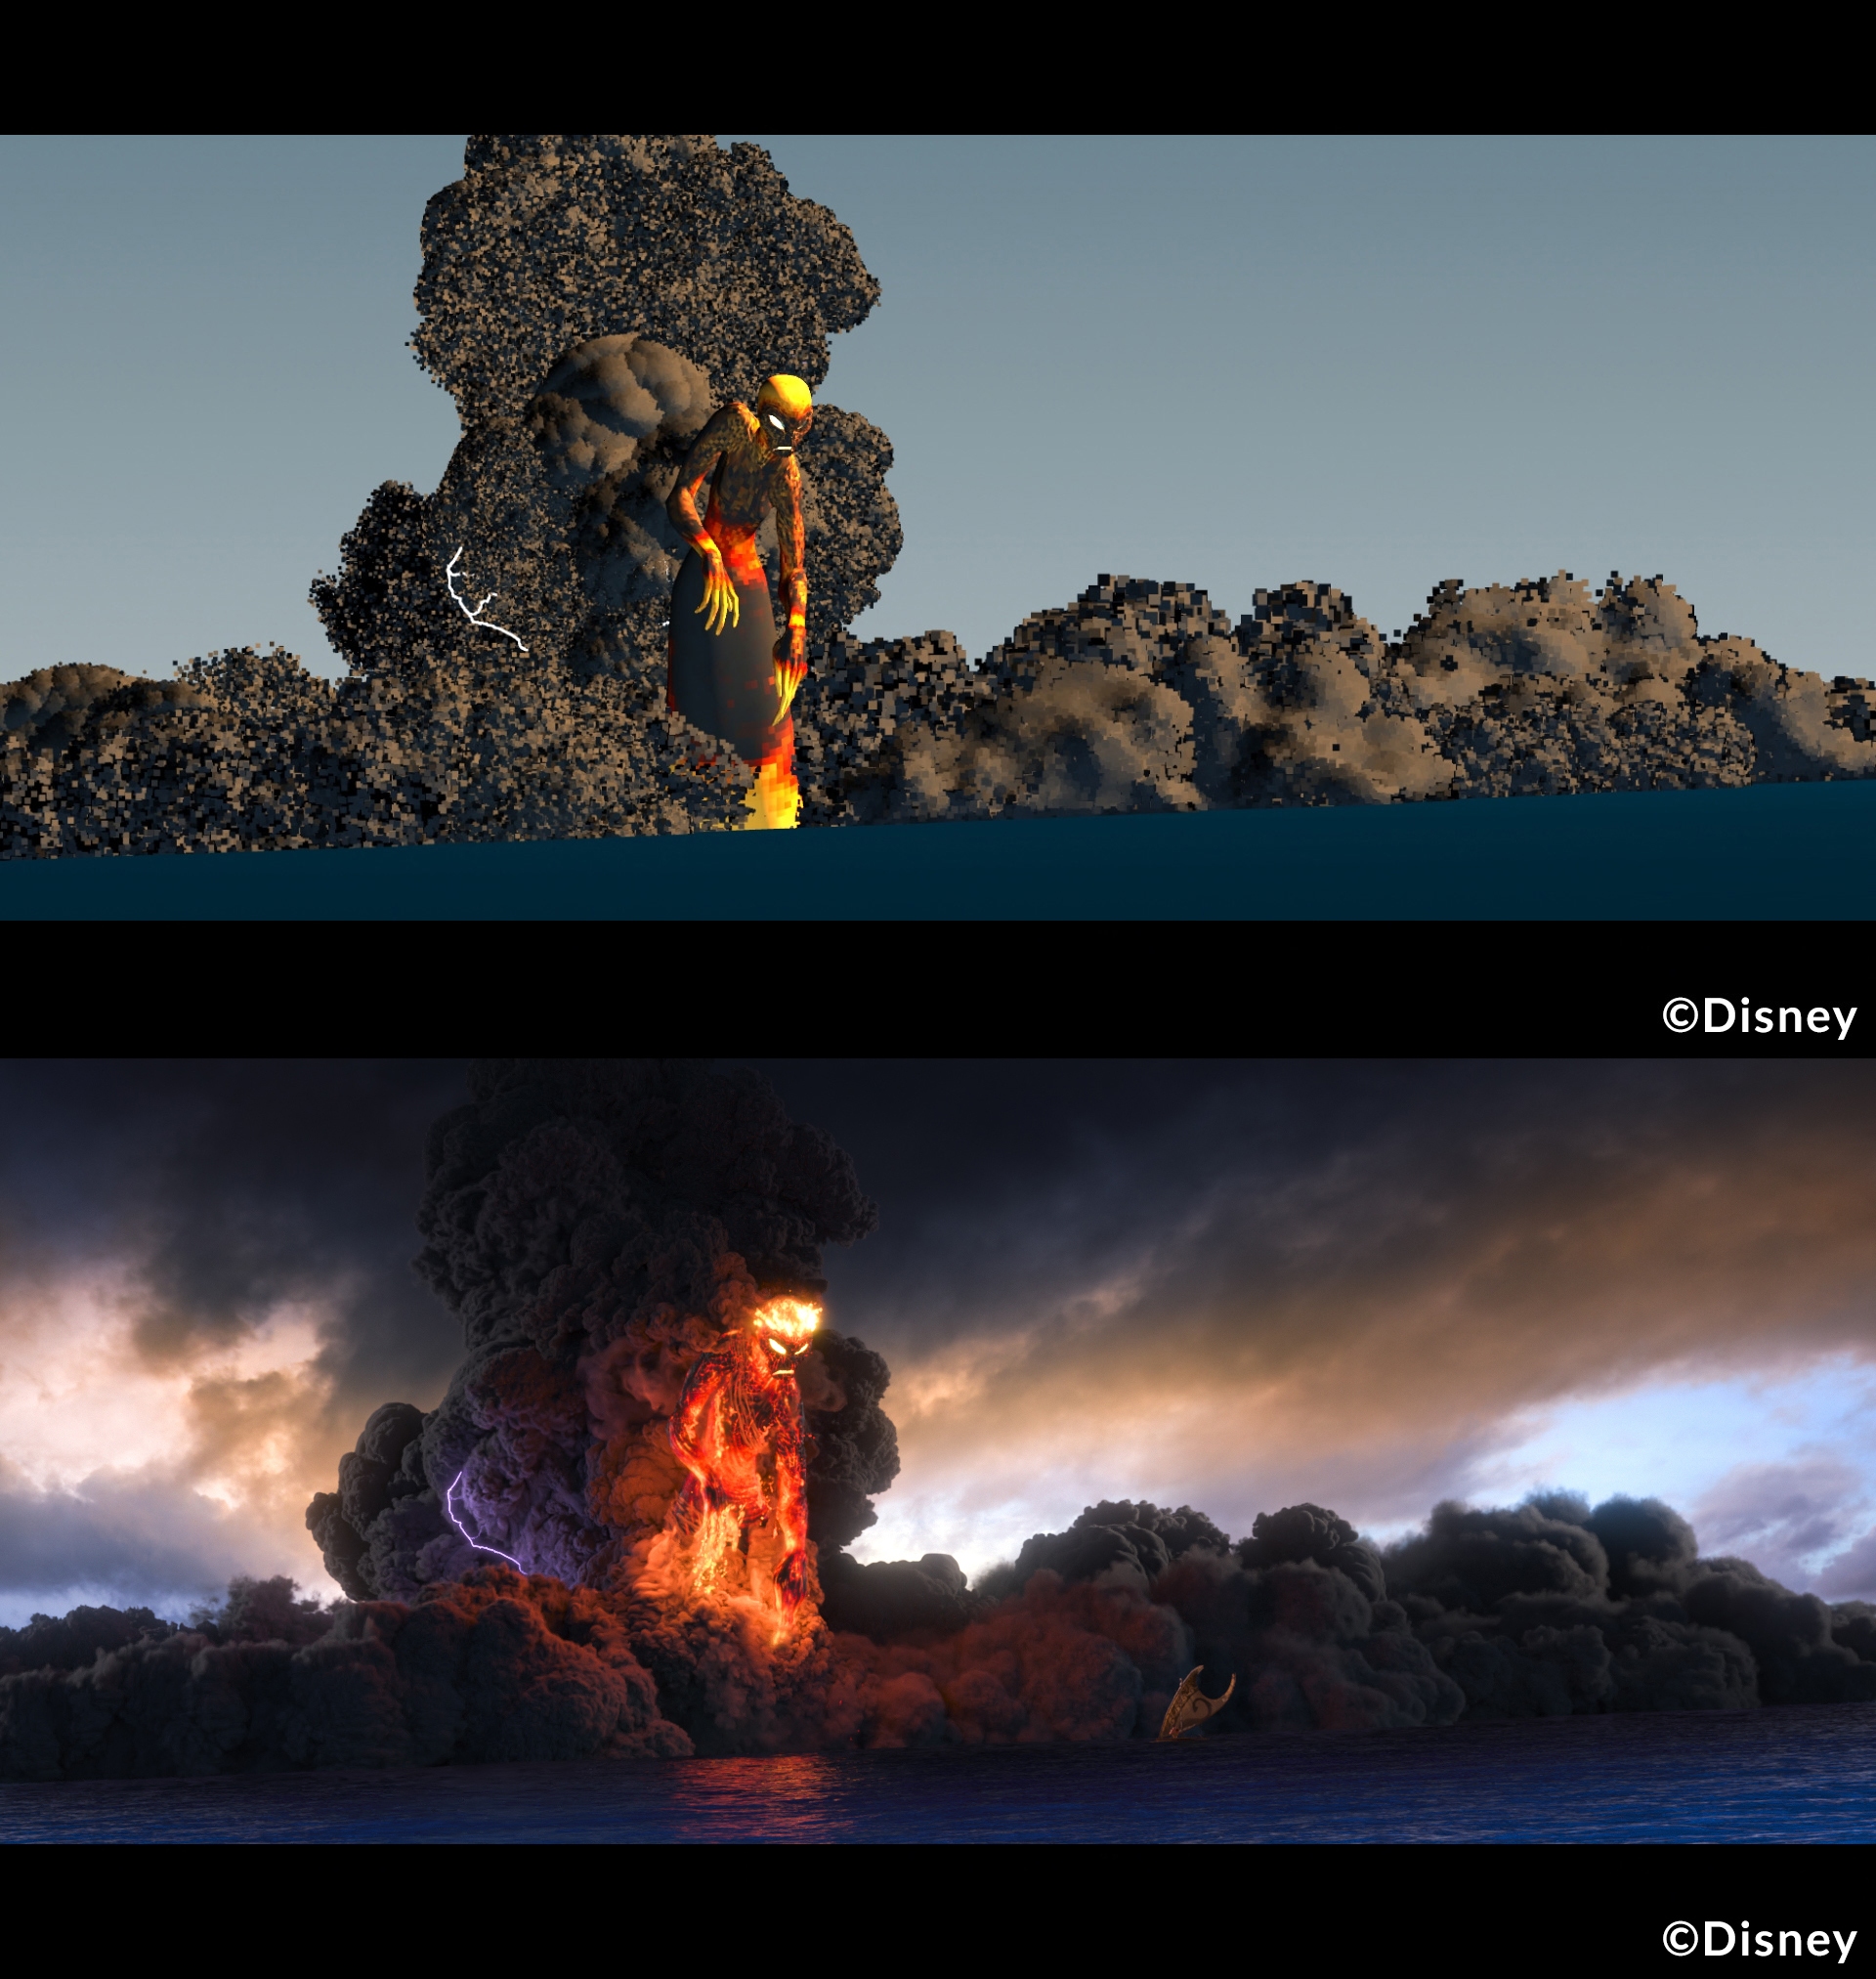
\includegraphics[width=12cm]{bilder/vaiana.jpg}
    \caption{Vorher-Nachher-Vergleich der Simulationen eines Shots aus dem Film \glqq Moana\grqq{} (2016).}
    \source{\citet[]{side-effects-software-2017}}
    \label{fig:moana}
\end{figure}



Wie lässt sich diese Definition jetzt in die Visual Effects Welt übertragen? Zwei Elemente sind hierfür wichtig: die Zeit und die auf ihr basierende Historie. Als Beispiel für den realen Prozess soll eine Explosion in 3D repliziert werden. Zu Beginn sei ein Emitter an einer bestimmten Position im 3D-Raum, der Schritt für Schritt Rauch und Flammen in den leeren Raum emittiert, über eine vom Nutzer bestimmte Zeit hinweg. Die Schritte sind in diesem Fall die einzelnen Bilder eines Films, auch \textit{Frames} genannt. Im ersten Frame ist die Explosion gering und hat viel Energie, die dafür sorgt, dass sich das Feuer und der Rauch ausbreiten können. Im zweiten Frame breitet sich die Explosion stark aus, während ihr Energielevel sinkt. Die Simulation entwickelt sich über mehrere Sekunden, bis ihre Energie aufgebraucht ist und die Flammen und der Rauch langsam verschwinden. Jeder Frame in einer Simulation muss auf dem Vorherigen aufbauen, damit der physikalisch korrekte Ablauf gewährt ist. Das bedeutet, dass dieses System von Frame zu Frame deterministischen Algorithmen unterliegt, also dass für dieselbe Eingabe stets dasselbe Ergebnis erzeugt wird. So lässt sich mit den vorhandenen Daten zur Energie immer vorhersagen, wie der nächste Frame aussehen wird. Bei einer 100 Frames langen Simulation ist es jedoch nicht möglich, erst den letzten Frame zu simulieren, denn es ist nicht bekannt, wie sich die Simulation in den 99 vorherigen Frames entwickelt hat. So bedarf es also einer Historie an Frames, die aufeinander aufbauen, aus der wir schlussfolgern können, wie sie sich für den 101 Frame entwickeln würde, wenn alle 100 Frames davor bereits simuliert wurden.\\

Solche Simulationen tragen erheblich zum Realismus eines Filmes bei, sind aber sehr aufwendig in ihrer Herstellung. Für die Visual Effects der Amazon Serie \textit{Star Treck Picard  (2020)}, unter anderem erstellt von Mackevison, wurde zum Beispiel ein auf einer Wassersimulation basierender Wurmloch-Effekt über mehrere Tage hinweg simuliert, um diesen später zu rendern und in einen Shot zu integrieren. Die Berechnung eines Frames dauerte im Schnitt acht Minuten und benötige 25 Gigabyte Speicherplatz. Für die insgesamt 750 Frames ergibt sich eine Simulationszeit von circa vier Tagen und ein Speicherplatzverbrauch von 18 Terabyte. Meistens ist eine Version einer Simulation nicht genug, sondern es werden einige Iterationen benötigt, um Verbesserungen und Kundenwünsche zu integrieren. So zeigt sich, dass es für ein Unternehmen im VFX-Bereich äußerst wertvoll ist, diese Prozesse zu beschleunigen und datensparsamer zu gestalten. Ein schnelleres Iterieren von Simulationen ermöglicht es dem Artist mehrere solcher Aufgaben in derselben Zeit zu bewältigen und Simulationen, die weniger Speicherplatz verbrauchen, würden eine große Kostenersparnis darstellen.

\section{Arten von Simulationen im VFX-Bereich}
Dieser Abschnitt soll einen Überblick über die verschiedenen Arten von Simulationen im VFX Bereich geben. Zuerst folgt ein Exkurs in den Aufbau und die Struktur eines 3D-Modells, denn die verschiedenen Simulationsarten gehen teilweise unterschiedlich mit dieser Struktur um. Die Erläuterungen beziehen sich stets auf die 3D-Simulations-Software \textit{Houdini} des Herstellers \textit{SideFX} \parencite[]{houdini}. Die Wahl Houdini als Programm für das Erzeugen der Simulationen zu nutzen, basierte auf dessen häufigen Einsatz in VFX-Unternehmen. Laut \citet[]{kim-2022} hat sich Houdini bei einer breiten Masse an Film- und VFX-Unternehmen etabliert. Auch Mackevision nutzt Houdini, um eine Vielzahl an Filmeffekten zu simulieren.

\begin{figure}[ht]
    \centering
    \includegraphics[width=8cm]{bilder/wireframe.jpg}
    \caption{Wireframe Ansicht eines 3D-Modells.}
    \source{Bild: Philipp Benner, Modell: Rico Cilliers}
    \label{fig:wire}
\end{figure}

\citet[]{menace-2021} nach, bestünden 3D-Modelle grundlegend aus Punkten, den sogenannten \textit{Vertices}, welche an bestimmten Koordinaten im dreidimensionalen Raum platziert seien. Um nun die Illusion eines geschlossenen Körpers zu erzeugen, würden drei oder vier Punkte miteinander verbunden, um eine Fläche zu schaffen. Drei Punkte würden ein Dreieck oder \textit{Triangle} und vier Punkten ein \textit{Quad} (eng. Quadrilateral für Viereck) erzeugen. Abbildung \ref{fig:wire} zeigt im mittleren Bildausschnitt das Modell als \textit{Mesh, Wireframe oder auch Drahtmodell} bestehend aus Quads. Letztlich werden die Punkte des Modells und die Verbindungslinien oder \textit{Edges} pro Punkt zu seinen Nachbarn gespeichert. Dies sind die grundlegenden Informationen, mit denen in den folgenden Simulationen gearbeitet wird.

\subsection{Rigid Body Simulations} 
Zu Deutsch \textit{Starrkörpersimulationen}. Sie werden verwendet, um Objekte zu bewegen oder sie mit anderen Objekten kollidieren zu lassen. Wie der Name schon andeutet, sind diese Objekte starr und nicht verformbar. Als Beispiel dient eine Bowlingkugel und Bowling-Pins auf einer Bahn. Die Kugel erhält eine initiale Geschwindigkeit in Richtung der Pins, rollt die Bahn entlang und kollidiert mit ihnen. Die Verbindungslinien der Punkte im Mesh behalten dabei stets ihre Länge und Rotation zueinander. Sollen die Objekte verformbar sein, so kommen \textit{Soft Body Simulations} zum Einsatz. Dabei lässt sich die Länge und Rotation der Edges zu den anderen Punkten verändern. So können sich Teile des Modells zusammenziehen, strecken und falten \parencite[]{baraff-2001}.

\subsection{Particle Simulations} 
Sie sind die simpelste Form der Simulationen. Dabei werden nur einzelne Punkte, ohne Edges oder Flächen simuliert. Durch Kräfte wie Wind, Gravitation oder Magnetismus wird ihre Bewegung im Raum über Zeit berechnet. Erhalten die Partikel noch ein Attribut wie eine Lebensspanne, lassen sie sich nach einer gewissen Zeit aus der Simulation entfernen oder langsam ausblenden. Meist haben die Partikel keine Größe während der Simulation und sind theoretisch gesehen unendlich klein \parencite[]{reeves}. Später, während des Renderings, also dem Errechnen des fertigen Bildes aus den 3D-Daten, wird an die Position eines Punktes eine winzige Kugel mit einem gewissen Radius gesetzt, um das Partikel im Bild sichtbar zu machen \parencite[]{sidefxparicle}. Viele magische Filmeffekte nutzen diese Art der Simulation, dann aber mit Millionen von Partikeln, um den Eindruck einer festen Materie zu erwecken.

\subsection{Pyro Simulations} 
Solche Simulationen nutzen eine gänzlich andere Struktur, um Flammen und Rauch zu simulieren. Dabei spielen Punkte und Edges keine Rolle mehr, sondern nutzen sogenannte \textit{Voxel}. Dieser Begriff leitet sich von \textit{Volume Elements} \parencite[S. 549]{FoleyDamEtAl90} ab und beschreibt einen Würfel, der ein Teil eines dreidimensionalen Rasters ist. Abbildung \ref{voxel} zeigt ein Pixelbild der Zahl 5. Anhand der Helligkeitswerte der Pixel ist erkennbar, dass einige Pixel den Wert eins haben, was bedeutet, dass sie zu 100\% weiß sind. Andere Pixel hingegen sind etwas dunkler und haben geringere Helligkeitswerte. Dieses Prinzip lässt sich von einem zweidimensionalen in ein dreidimensionales Raster übertragen und es entsteht ein sogenanntes \textit{Voxel Grid}, zu sehen links unten in Abbildung \ref{voxel}. Für jeden Voxel wird anstatt des Helligkeitswertes nun ein Wert verwendet, der angibt, wie transparent, oder dicht der Voxel ist – \textit{Density} genannt –  und das Modell erhält somit eine dreidimensionale Struktur, die teilweise durchsichtig ist. In Abbildung \ref{voxel} rechts unten zu sehen: Das normale 3D-Modell und die teilweise durchsichtige Voxel-Struktur. \\

\begin{figure}[ht]
    \centering
    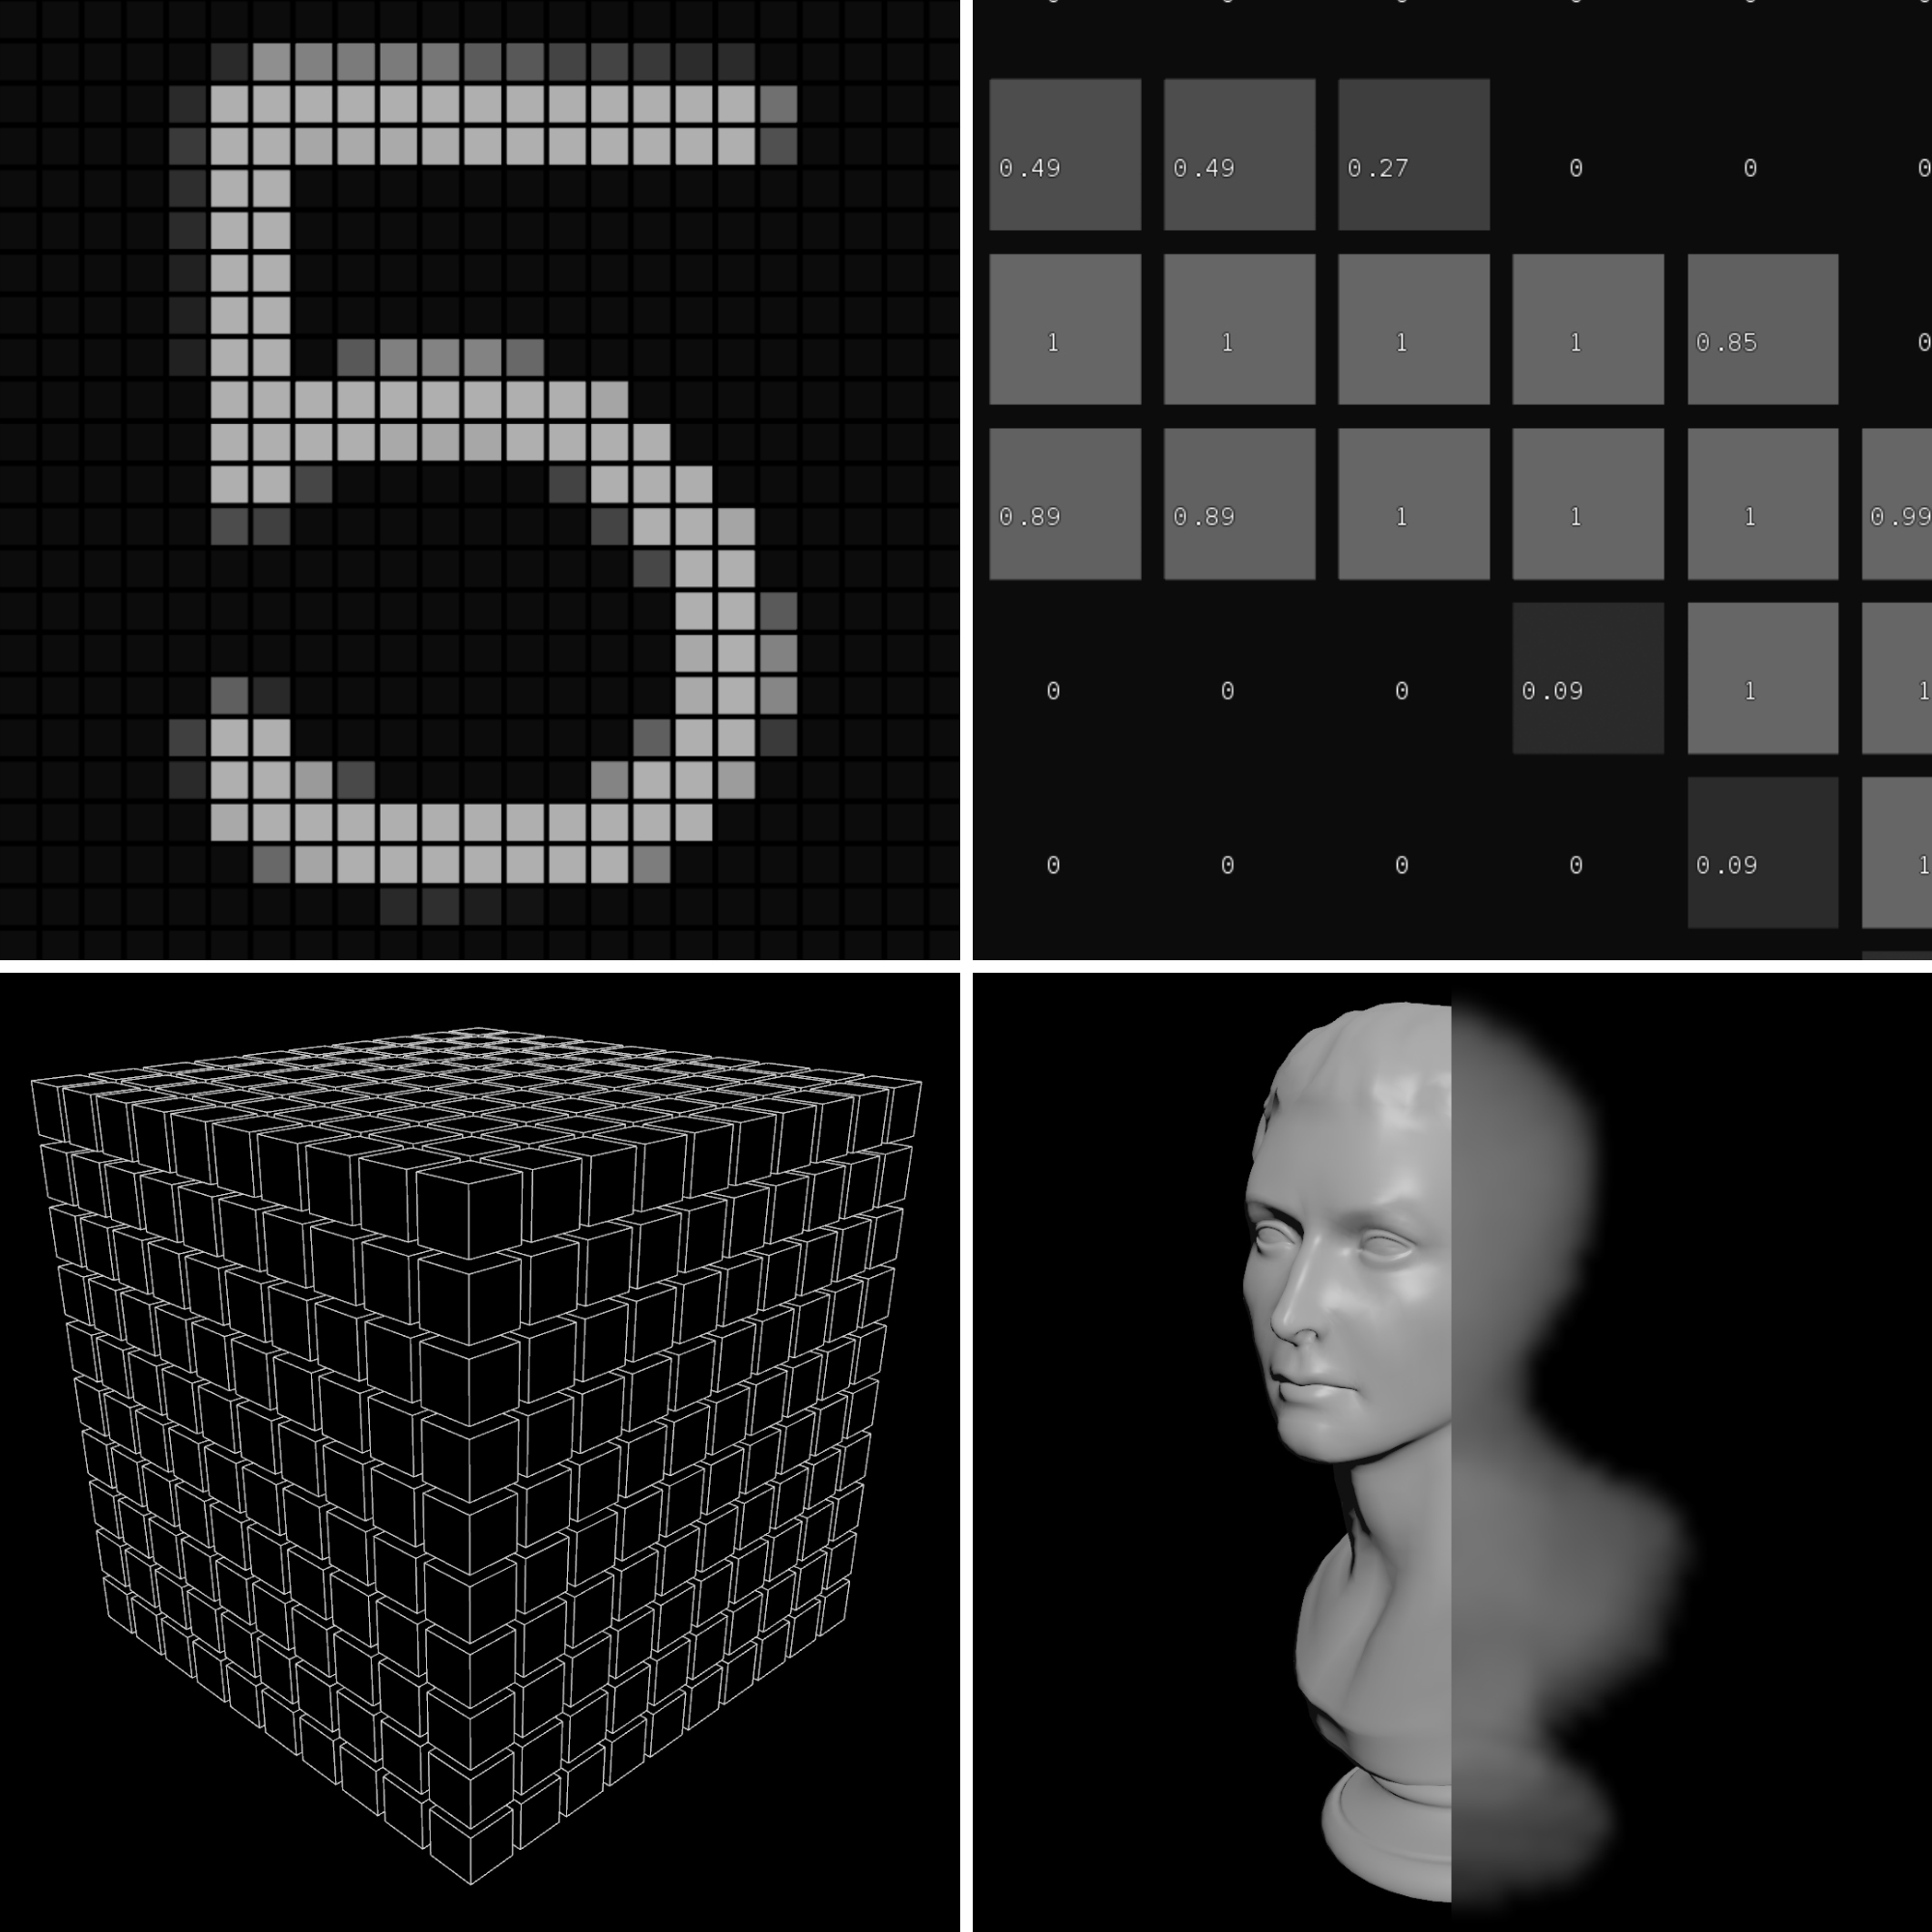
\includegraphics[width=10cm]{bilder/voxel.jpg}
    \caption{Aufbau eines Voxel Grids.}
    \source{Bild: Philipp Benner, Modell: Rico Cilliers}
    \label{voxel}
\end{figure}

Um nun Rauch oder Flammen zu simulieren, wird neben der Transparency noch einen \textit{Velocity} Wert in jedem Voxel gespeichert. Er besteht aus einem Vektor, der angibt, in welche Richtung sich der Voxel mit welcher Stärke bewegen würde, auch \textit{Advektion} genannt. Diese Werte werden während des Simulierens erzeugt und in \textit{Fields} gespeichert, wie etwa das Density und Velocity Field. Während einer Pyro-Simulation wird nun für jeden Voxel berechnet, in welche Richtung sich seine Density - basierend auf der Velocity - Frame für Frame verschiebt. Die Velocity wird dabei mit verschoben und nimmt zu oder ab, je nachdem welche physikalischen Kräfte für die Simulation eingestellt wurden. In der 3D-Simulations-Software Houdini, lassen sich komplexe Pyro-Simulationen mit weiteren Fields realisieren. Wie etwa mit dem \textit{Temperature Field}, welches die Hitzeverteilung in der Simulation speichert. Rauch oder Flammen in heißen Bereichen steigen somit schneller in der Luft auf und verteilen sich \parencite[]{understandinghowpyroworks}. Um nun eine realistisch aussehende Simulation mit vielen Details zu erhalten, muss die Anzahl an Voxel überaus hoch sein und erreicht dabei meistens den Millionenbereich.


\subsection{Water Simulations} 
Sie sind eine Mischform aus Partikel- und Pyro-Simulationen, in Houdini genannt \textit{FLIP Fluids} \parencite[]{flipsolver}. Die Partikel nehmen dabei die Rolle von Wassertropfen in der Simulation ein. Alle Informationen wie etwa die Größe, Geschwindigkeit und die Lebensspanne werden in den Partikeln gespeichert. Nur für die Berechnung der Strömung auf Grundlage der Navier-Stokes Gleichungen werden diese Informationen kurzzeitig in ein Volume übertragen \parencite[]{AlexandreJoelChorin.1967}. Dabei handelt es sich um ein Velocity Field, welches dafür sorgt, dass sich die einzelnen Partikel räumlich besser verteilen und nicht alle in dieselbe Richtung wandern \parencite[]{flipsolver}. Die Partikel lassen sich dann mit den üblichen Kräften steuern, welche auch für die einfache Partikelsimulation genutzt werden.

\section{Dateiformat OpenVDB}
Für Simulationen, die nicht auf Voxel basieren, sondern wie etwa bei Particle Simulations, lässt sich bei errechneten Frames die Position der Punkte und weitere Attribute wie Edges, Partikelgröße oder die Lebensspanne pro Partikel speichern. \\

Da Voxel hingegen Teil eines dreidimensionalen Rasters sind, müsste eine 3D-Matrix pro Field gespeichert werden, da jedes Field einen anderen Wertetyp haben kann. Die Density eines Voxels wird etwa als eindimensionale Floating Point Nummer gespeichert, das Velocity Field speichert aber einen 3D-Vektor pro Voxel, da hierbei eine Richtung angezeigt werden muss. Dabei entsteht das Problem, dass innerhalb einer Pyro-Simulation oft viele Voxel existieren, die keine wichtigen Informationen beinhalten. Zum Beispiel befindet sich am Rand einer Explosion oftmals leerer Raum, an dem keine Density oder Velocity Werte vorhanden sind. Die gespeicherte 3D-Matrix würde also aus vielen Nullen bestehen und somit unnötigen Speicherplatz verbrauchen.\\

Um diesem Problem entgegenzutreten, nutzt Houdini unter anderem das weitverbreitete Dateiformat \textit{OpenVDB} \parencite[]{openvdb}, um Voxel zu speichern \parencite[]{volumesopenvdb}. Dabei werden mithilfe der Datenstruktur eines $B^{+}$-Baumes nur Voxel zur Speicherung aktiviert, in denen auch nützliche Informationen zu finden sind. Dieses Dateiformat ermöglicht es, die Daten kompakt zu speichern und sie schnell wieder einzulesen. Beispielsweise benötigen OpenVDB Volumes 50\% weniger Speicherplatz im RAM und 13-25\% weniger Platz auf der Festplatte, als andere, für diesen Zweck optimierte Dateiformate \parencite[S. 27:18]{10.1145/2487228.2487235}.

\section{Optimierung von Simulationen}
Es existieren also eine Vielzahl an komplexen Vorgängen, die beim Simulieren eine Rolle spielen. Es gibt verschiedene Techniken, die für bestimmte Arten von Simulationen zum Einsatz kommen, welche mit teilweise gänzlich anderen Datenstrukturen arbeiten. Eine Simulation anzufertigen kann Tage dauern und sie verbraucht ebenso mehrere Terabyte Festplattenspeicher.\\

Da Visual Effects und die damit einhergehenden Simulationen in Zukunft weiterhin eine große Rolle spielen werden, steht die Forschung in diesem Bereich nicht still. Auch die steigende Leistung von Computerhardware bietet neue Möglichkeiten. Mittlerweile lassen sich Simulationen teilweise schneller und effizienter auf einer Grafikkarte anstatt dem Prozessor berechnen. Für Simulationen in geringer Auflösung ist dies sogar schon in Echtzeit möglich \parencite[S. 9]{Real-Time-incompressible}.\\

Forscher untersuchen unter anderem auch stetig, wie mit künstlicher Intelligenz Simulationen optimiert werden können. Es gelang ihnen etwa, eine künstliche Intelligenz so zu trainieren, dass sie die physikalischen Gesetze der echten Welt berücksichtigt \parencite[]{physicsinformed}. Einer anderen Gruppe ist es gelungen, Flüssigkeiten mit einem Deep Neural Network zu simulieren \parencite[]{deepfluid}. Beide Forschungsarbeiten bieten große Vorteile, da sie auf Simulationssoftware mit komplexen Algorithmen verzichten und das neuronale Netz trotzdem in der Lage ist, erstaunliche Ergebnisse zu liefern. \\

%    \chapter{Künstliche Intelligenz}
\thispagestyle{fancy}
\section{Definition: künstliche Intelligenz}
Um den Begriff der künstlichen Intelligenz besser verstehen zu können, soll zunächst allgemein festgehalten werden, was Intelligenz bedeutet. Obwohl die Intelligenz ein abstraktes, gesellschaftliches Konstrukt ist, lässt sie sich wie folgt definieren:

\begin{quote}
\glqq  Intelligenz ist die Fähigkeit, aus Erfahrung zu lernen, Probleme zu lösen und das Wissen zur Anpassung an neue Situationen einzusetzen.\grqq{} \parencite[S. 400]{psychologie}
\end{quote}

Das Ziel mit einer künstlichen Intelligenz soll nun also sein, dass ein Computer diese Fähigkeit erlernt. Somit lässt sich künstliche Intelligenz als Teilgebiet der Informatik definieren, welches sich mit der Erforschung von Mechanismen des intelligenten menschlichen Verhaltens befasst. Dies geschieht durch Simulation mithilfe künstlicher Artefakte. Diese Artefakte sind für gewöhnlich Programme auf einem Computer \parencite[]{wichert}. Nach \citet[23]{russell2012knstliche} lässt sich dieses Teilgebiet weiter in vier Kategorien aufteilen:\\

\begin{enumerate}
    \item \textbf{Menschliches Denken}
    \item[] Der Computer soll in der Lage sein zu denken. Dabei soll er die Fähigkeit haben, Entscheidungen treffen zu können, Probleme zu lösen und sich eigenständig neues Wissen aneignen.
    
    \item \textbf{Menschliches Handeln}
    \item[] Mit den Fähigkeiten des menschlichen Denkens soll es dem Computer möglich sein, diese Dinge aktiv umsetzen zu können. Er handelt aktiv, nachdem er eine Entscheidung getroffen hat oder versucht aktiv ein Problem zu lösen.
    
    \item \textbf{Rationales Denken}
    \item[] Der Computer soll ein allgemeines, logisches Denken erlernen können, das auf mathematischen Formalismen basiert. Dies geschieht mittels programmiertechnischer Modelle und befähigt ihn zu logisch zu schließen und zu agieren.
    
    \item \textbf{Rationales Handeln}
    \item[] Er werden sogenannte \textit{rationale Agenten erzeugt}, also technische Operatoren, die aktiv handeln können. Sie haben das Ziel, immer das beste Ergebnis zu erzielen \parencite[S. 25]{russell2012knstliche}.
\end{enumerate}


Es sollen also Systeme entstehen, die so denken und agieren wie Menschen und ebenso rational denken und agieren wie sie. Dafür werden rationale Agenten geschaffen, die aus diesen Eigenschaften hervorgehen und entsprechend handeln.

\section{Ebenen der künstlichen Intelligenz}
Auch innerhalb der künstlichen Intelligenz lassen sich verschiedene Ebenen ausmachen, etwa die Begriffe des \textit{Machine Learnings} oder \textit{Deep Learnings}. \citet[]{copeland_2021} erklärt, dass die beiden Begriffe aus der Entwicklung der künstlichen Intelligenz entstanden seien, denn Deep Learing sei eine weitere Ebene, welche sich innerhalb von Machine Learning entwickelte (Abbildung \ref{KIKreise}). Obwohl die Konzepte des Deep Learnings genauso alt sind, wie die des Machine Learnings, sei es erst seit wenigen Jahren möglich, sie in großem Maße einzusetzen. Der Autor hält fest, dass die zu dem Zeitpunkt benötigte Computerleistung, wie etwa schnelle GPUs, damals nicht existierte. Der größte Unterschied zwischen Machine und Deep Learning seien die sogenannten \textit{neuronalen Netze} des Deep Learnings.\\

\begin{figure}[ht]
    \centering
    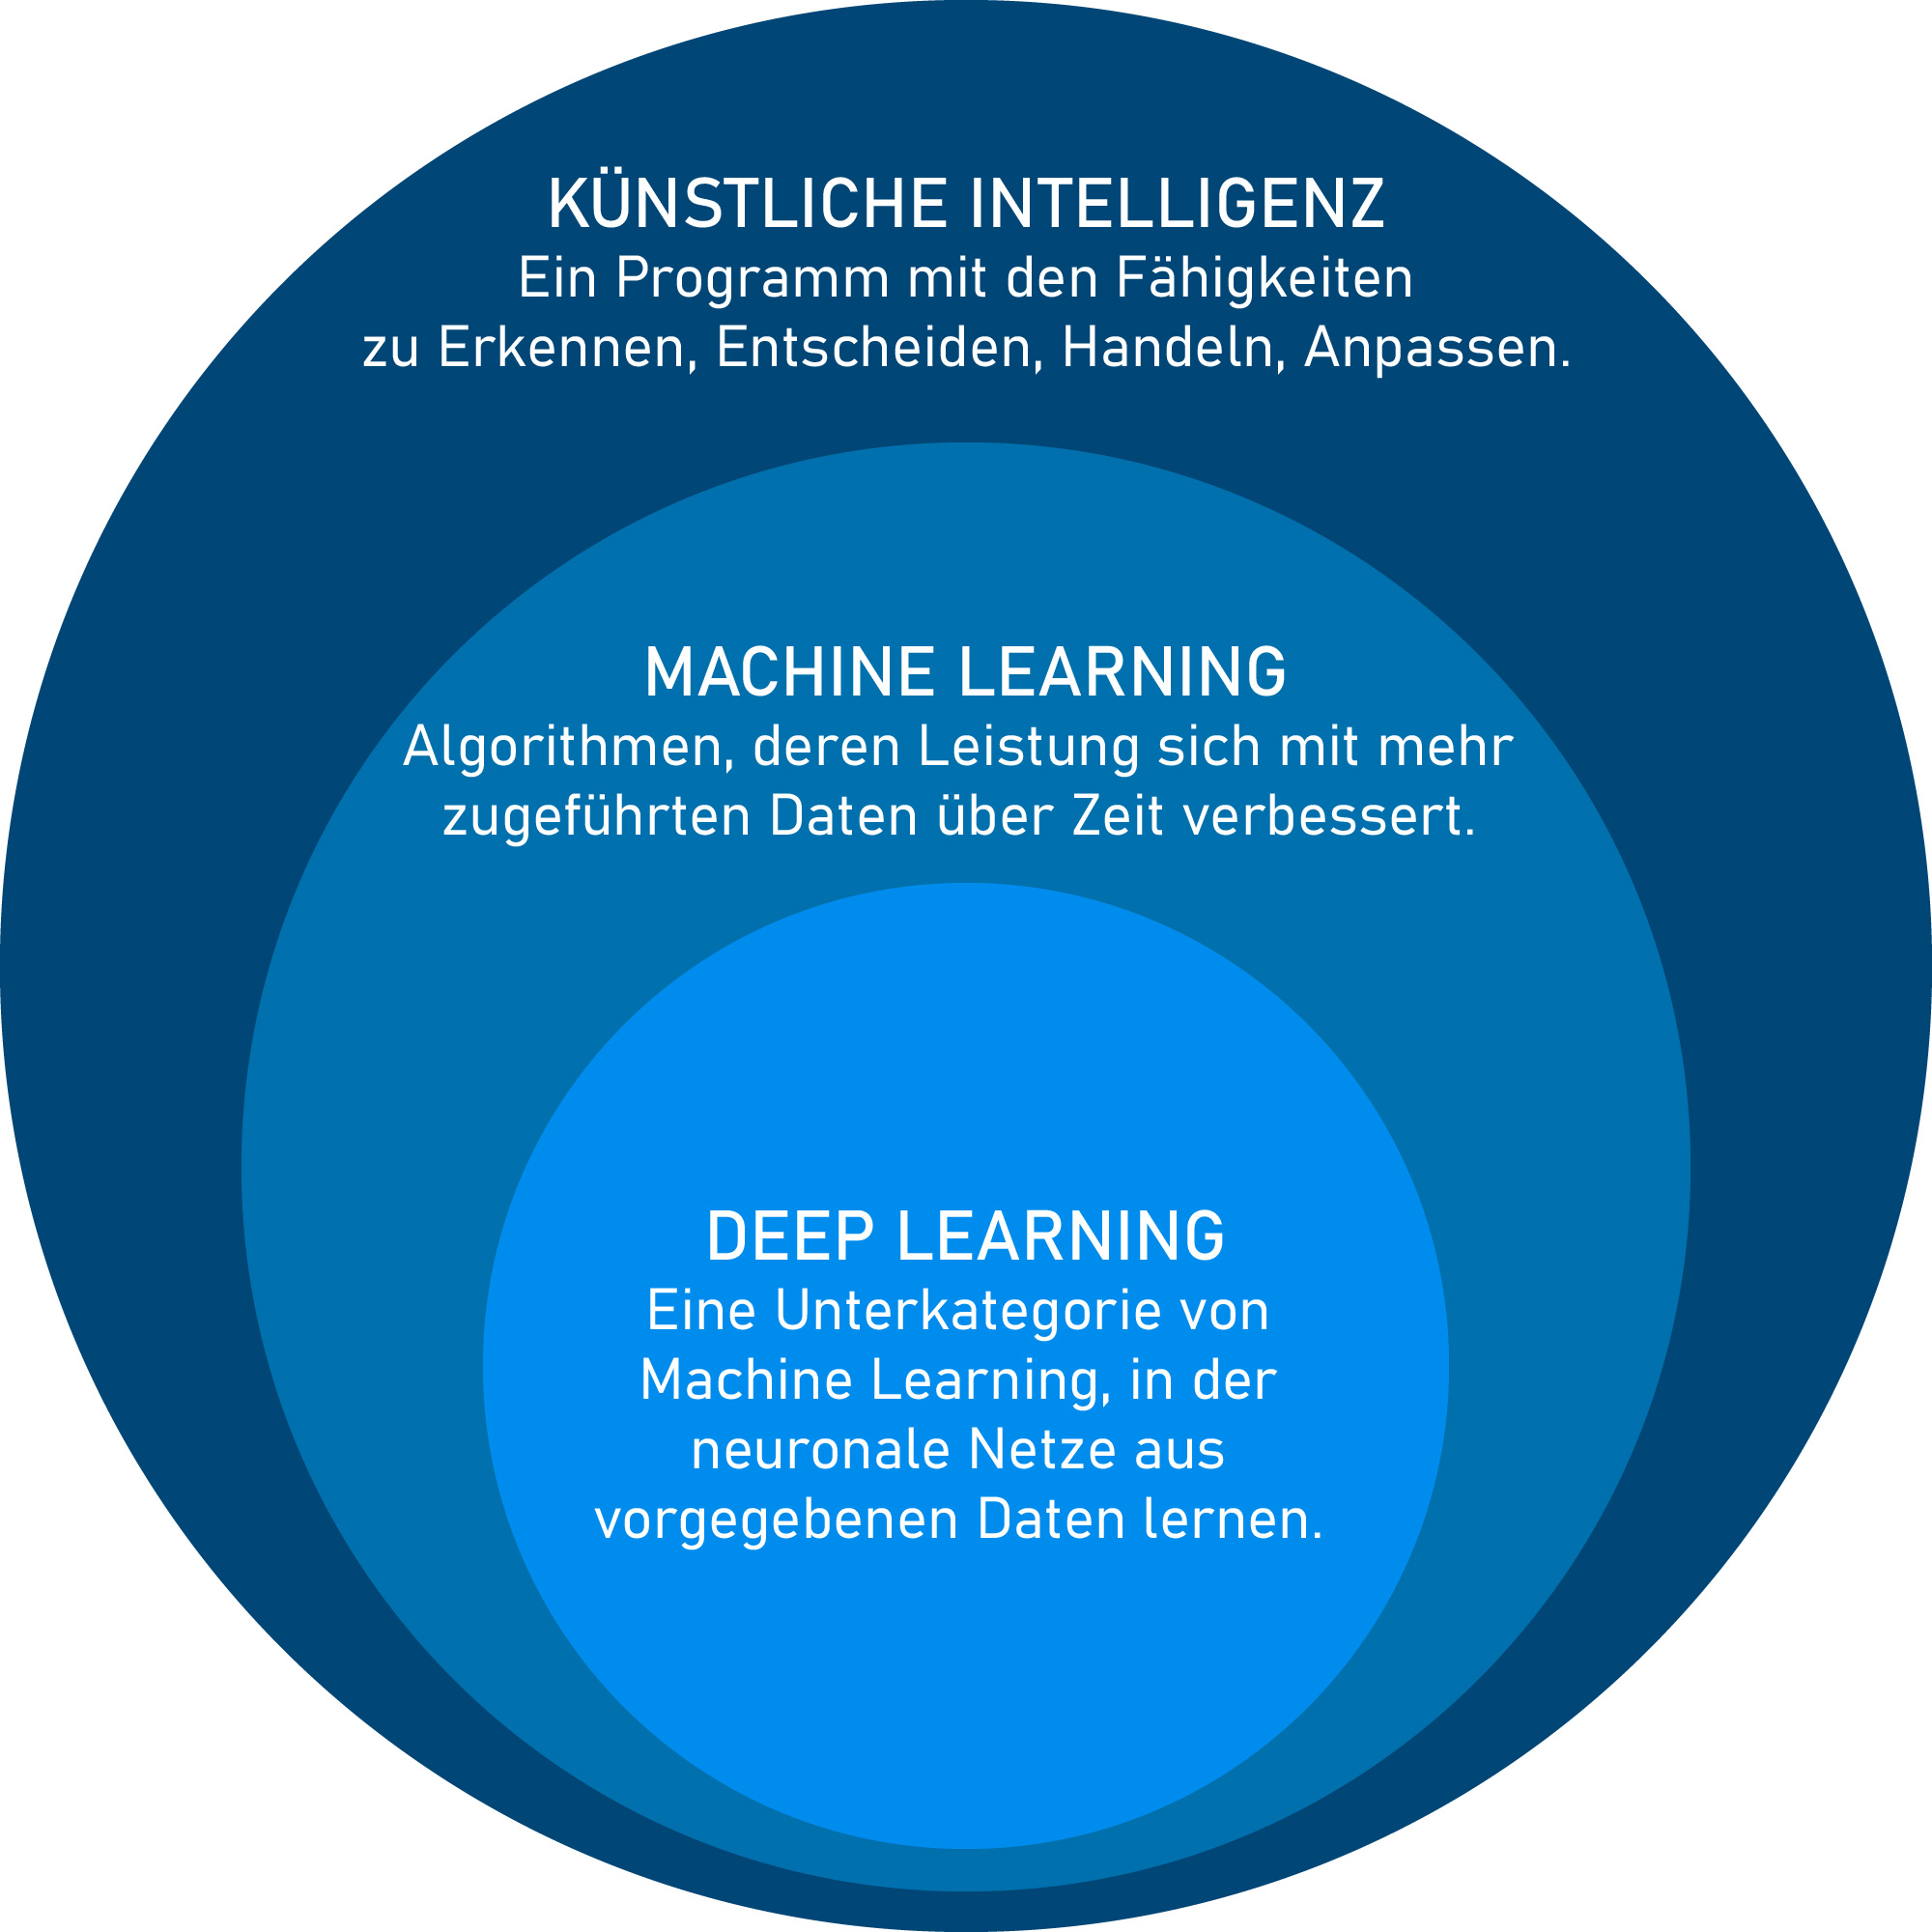
\includegraphics[width=8cm]{bilder/KIKreise2.jpg}
    \caption{Ebenen der künstlichen Intelligenz.}
    \source{Philipp Benner in Anlehnung an \citet[]{wuttke_2022}.}
    \label{KIKreise}
\end{figure}

\citet[]{Janiesch.2021} erklären, dass Machine Learning vom Menschen vorgegebene Merkmale nutze, um einem Algorithmus beizubringen, welche Elemente in den vorliegenden Daten eine hohe Relevanz haben und das Ergebnis beeinflussen würden. Erhält der Algorithmus Daten, so könne dieser mithilfe der Merkmale über eine gewisse Zeit hinweg selbstständig lernen und seine Funktion verbessern. Dieses Definieren der Merkmale nannten die Autoren \textit{Feature Engineering}. Soll zum Beispiel festgestellt werden, wie hilfreich eine Bewertung in einem Online-Shop ist, ließe sich als Merkmal die Wortwahl, oder die Anzahl der Wörter nehmen. \\

Ebenso wird nach \citet[]{Janiesch.2021} kein Feature Engineering beim Deep Learning verwendet. Dort hingegen kommen neuronale Netze zum Einsatz, die wie im menschlichen Gehirn auf vielen miteinander verbundenen Neuronen basieren. Die Neuronen lernen selbstständig, welche Merkmale ein positives oder negatives Ergebnis verursachen. Somit bietet der Einsatz von Deep Learning Netzen einen Zeitvorteil und es ist möglich, dass die Netze Merkmale erlernen, die ein Mensch während des Feature Engineerings nicht beachtet hat. Die genaue Arbeitsweise von neuronalen Netzen folgt im nächsten Abschnitt.\\

Mittlerweile sind die Konzepte des Deep Learnings ein essenzieller Forschungsbereich innerhalb künstlicher Intelligenzen. Das zeigt beispielsweise, dass das meist zitierte Whitepaper in der Kategorie \textit{Computer Vision and Pattern Recognition} im Jahr 2020, eines aus der Forschung an Deep Learning Netzwerken ist. Mit dem Titel \textit{Deep Residual Learning for Image Recognition}, publiziert durch ein Forscherteam bei Microsoft \parencite[]{crew2020}, wurde dargelegt, wie mit speziellen neuronalen Ebenen in einem Deep Learning Netzwerk das Lernverhalten des Netzes verbessert werden könnte.


\section{Einführung in neuronale Netze}
Im weiteren Verlauf dieser Arbeit sollen tiefergehende Einblicke in Deep Learning und neuronale Netzen gegeben werden. Dazu wird primär die Literatur des Autors \textit{Tariq Rashid} verwendet. Er ist ein qualifizierter Datenanalyst und publizierte einige Bücher über neuronale Netze und Algorithmen \parencite[]{educative-no-date}. Außerdem besitzt er einen Master of Science in Künstlicher Intelligenz sowie einen weiteren Master in Naturwissenschaften \parencite[]{linkedin-no-date}.\\

\citet[S. 32]{traiq_neuron} erklärt, dass Deep Learning versuche, sich die Funktionsweise des menschlichen Gehirns zunutze zu machen, indem einzelne Neuronen erschaffen, ein elektrisches Eingangssignal übernehmen und ein anderes Signal ausgeben würden, so zu sehen in Abbildung \ref{neuronen2}.


\begin{figure}[ht]
    \centering
    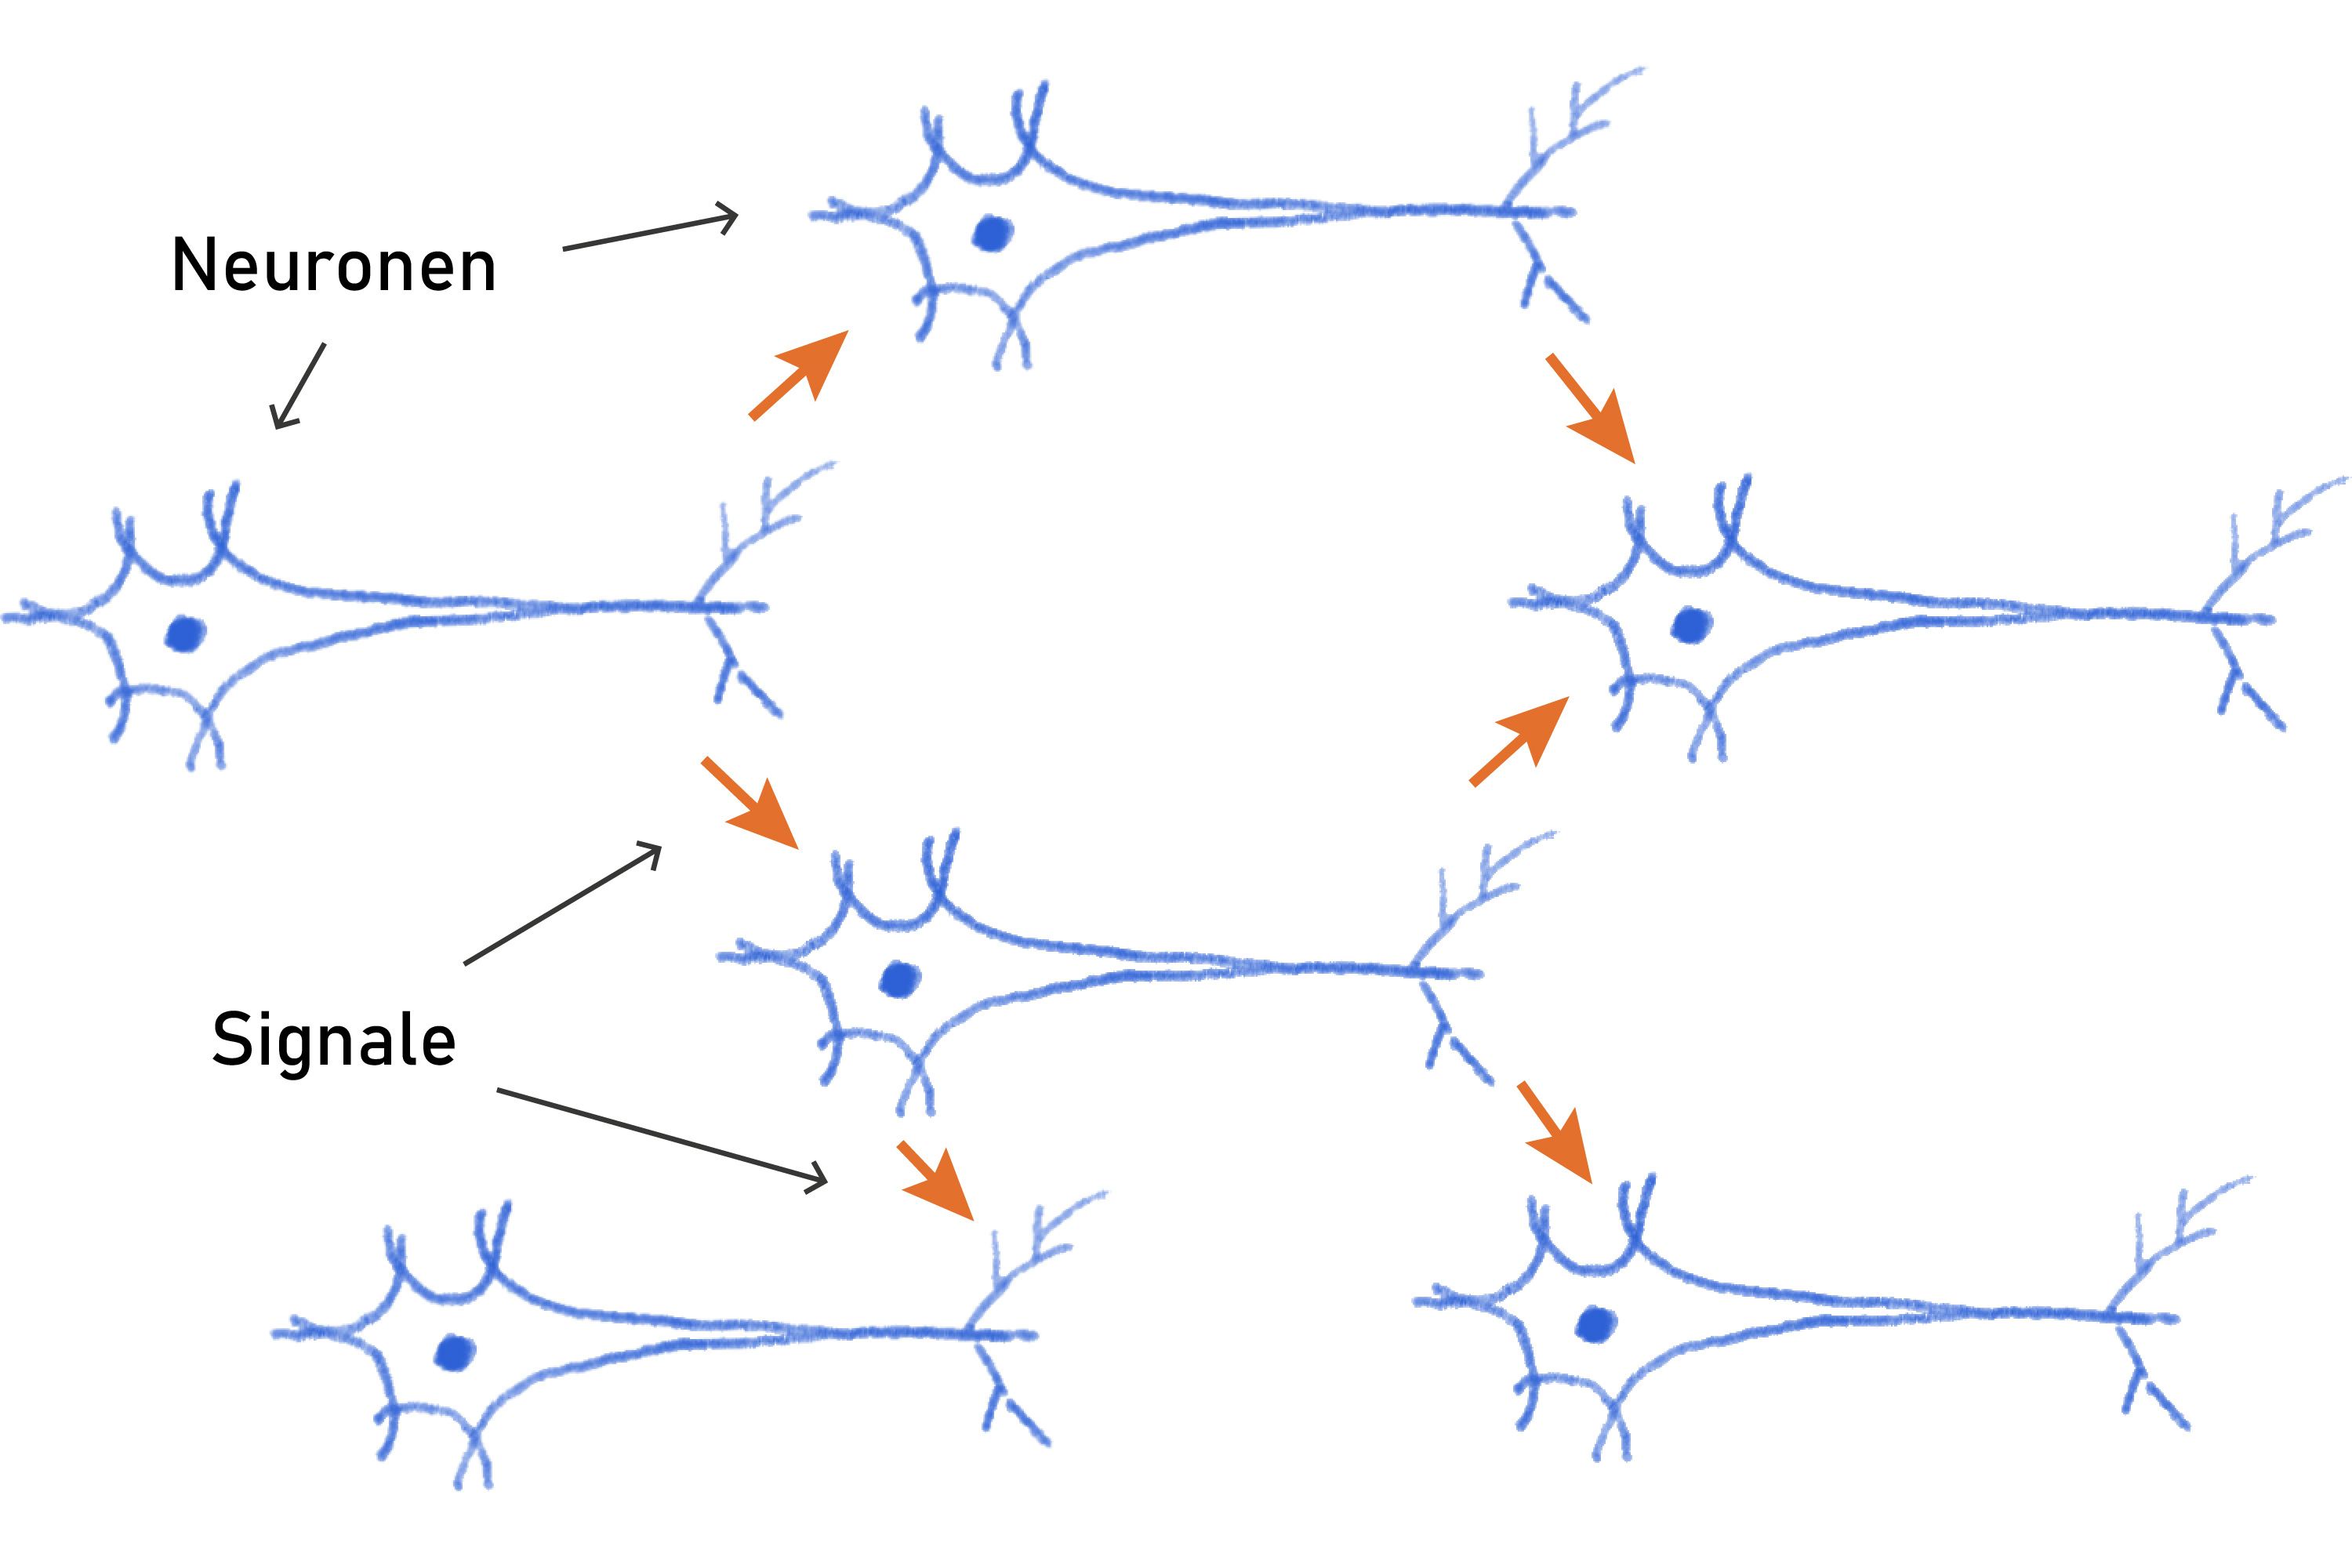
\includegraphics[width=10cm]{bilder/NeuronenGehirn.jpg}
    \caption{Darstellung eines neuronalen Netzes im menschlichen Gehirn.}
    \source{Philipp Benner in Anlehnung an \citet[36]{traiq_neuron}}
    \label{neuronen2}
\end{figure}

 Der Autor führt fort, dass die Eingangssignale jedoch nicht direkt wieder ausgegeben würden, sondern einen gewissen Schwellenwert überschreiten müssten, bevor eine Ausgabe erzeugt werden würde. Im Gehirn findet sich eine Vielzahl solcher Neuronen, deren Ein- und Ausgänge miteinander verbunden seien. So ist ein Neuron beispielsweise mit drei weiteren Neuronen in seinen Eingängen verbunden und erzeugt erst ein Ausgabesignal, wenn mindestens zwei der drei Eingänge ein elektrisches Signal erhalten. Dieses Konzept lässt sich ebenso digital abbilden und ist der Grundstein für künstliche neuronale Netze. Im Folgenden soll die Bezeichnung \textit{neuronales Netz} für das künstliche, digitale Netz in einem Computerprogramm stehen.\\

\section{Aufbau und Funktion neuronaler Netze}

Wie hilft ein solches Netz nun, menschliches Denken zu imitieren? Im Folgenden soll die Arbeitsweise eines neuronalen Netzes an einem vereinfachten Beispiel erklärt werden. Das neuronale Netz soll anhand eines Graustufenbildes erkennen, ob ein Hund auf einem Bild zu finden ist. Ein Ausgangswert zwischen 0,0 und 1,0 soll anzeigen, wie sicher sich das Netz ist, einen Hund erkannt zu haben. 0,0 bedeutet kein Hund, 1,0 bedeutet, das Netz ist sich sicher, einen Hund erkannt zu haben. Um das Netz zu verstehen, werden im Folgenden Begriffe zum Verständnis der Abbildung \ref{neuronalesnetz} erklärt.\\

\begin{figure}[ht]
    \centering
    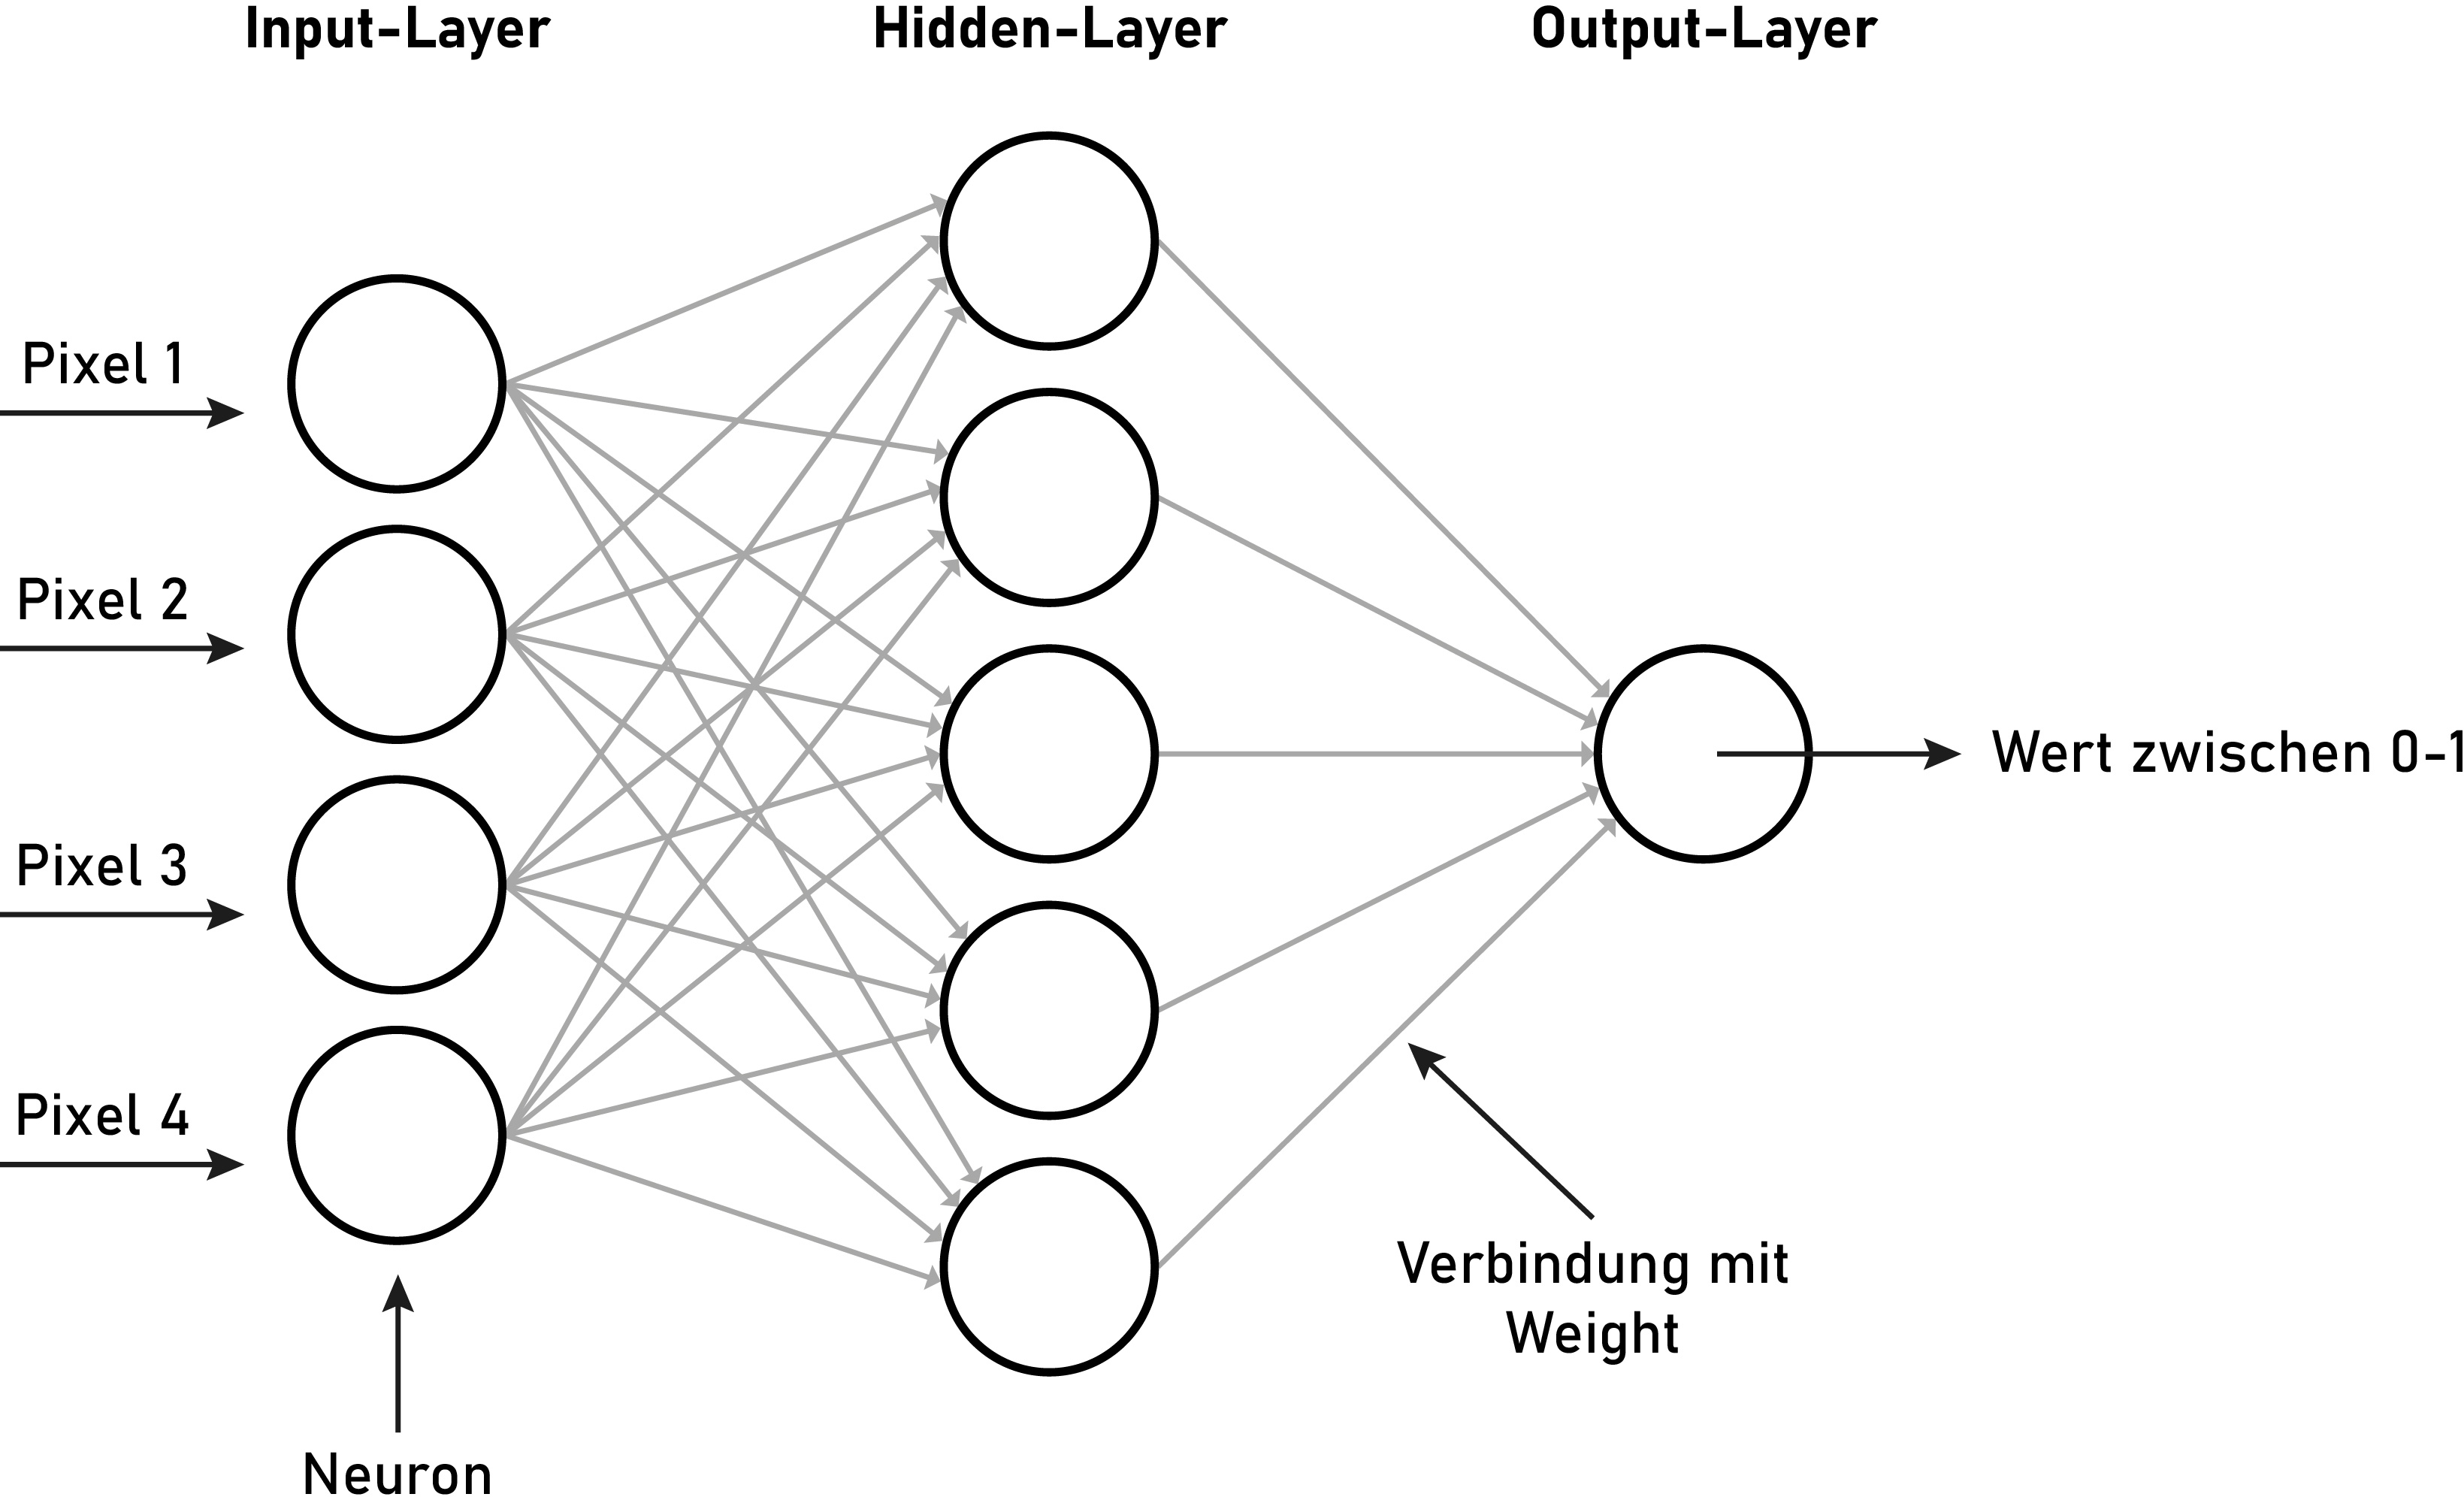
\includegraphics[width=11cm]{bilder/kuentlNetz.jpg}
    \caption{Darstellung eines künstlichen neuronalen Netzes.}
    \source{Philipp Benner}
    \label{neuronalesnetz}
\end{figure}

\subsubsection*{Neuron} Ein Neuron stellt einen Knotenpunkt im Netz dar. Es ist mit weiteren Neuronen durch seine Ein- und Ausgänge verbunden. Durch die Verbindungen fließen nun aber keine elektrischen Signale, sondern Zahlen. Am Ende einer jeden Verbindung steht ein Zahlenwert, der mit allen weiteren Verbindungen, die an einem Neuron anliegen, summiert und in die \textit{Activation Function} eingesetzt wird. Diese Funktion erzeugt einen einzelnen Ausgangswert pro Neuron, welcher wiederum über die Verbindungen an andere Neuronen weitergegeben wird \parencite[S. 40]{traiq_neuron}.

\subsubsection*{Activation Function} Zu Deutsch \textit{Aktivierungsfunktion}. Abbildung \ref{stufenfunktion} zeigt eine Stufenfunktion innerhalb eines Neurons. Alle Zahlenwerte am Eingang des Neurons werden summiert und müssen einen bestimmten Schwellenwert überschreiten. Erst dann wird der Ausgabewert von 0,8 erzeugt. Weitere Aktivierungsfunktionen sind zum Beispiel die nach \citet{Hahnloser2000} bei positiven Werten linear ansteigende \textit{ReLU} Funktion, bei der das Ausgabesignal denselben Wert hat wie das Eingabesignal, wenn das Eingabesignal größer als Null ist. Die S-Artige Sigmoidfunktion sei eine weitere wichtige Aktivierungsfunktion laut \citet[S. 34]{traiq_neuron}. Sie sei einfach zu berechnen und unterdrücke zu niedrige Eingangssignale.

\begin{figure}[ht]
    \centering
    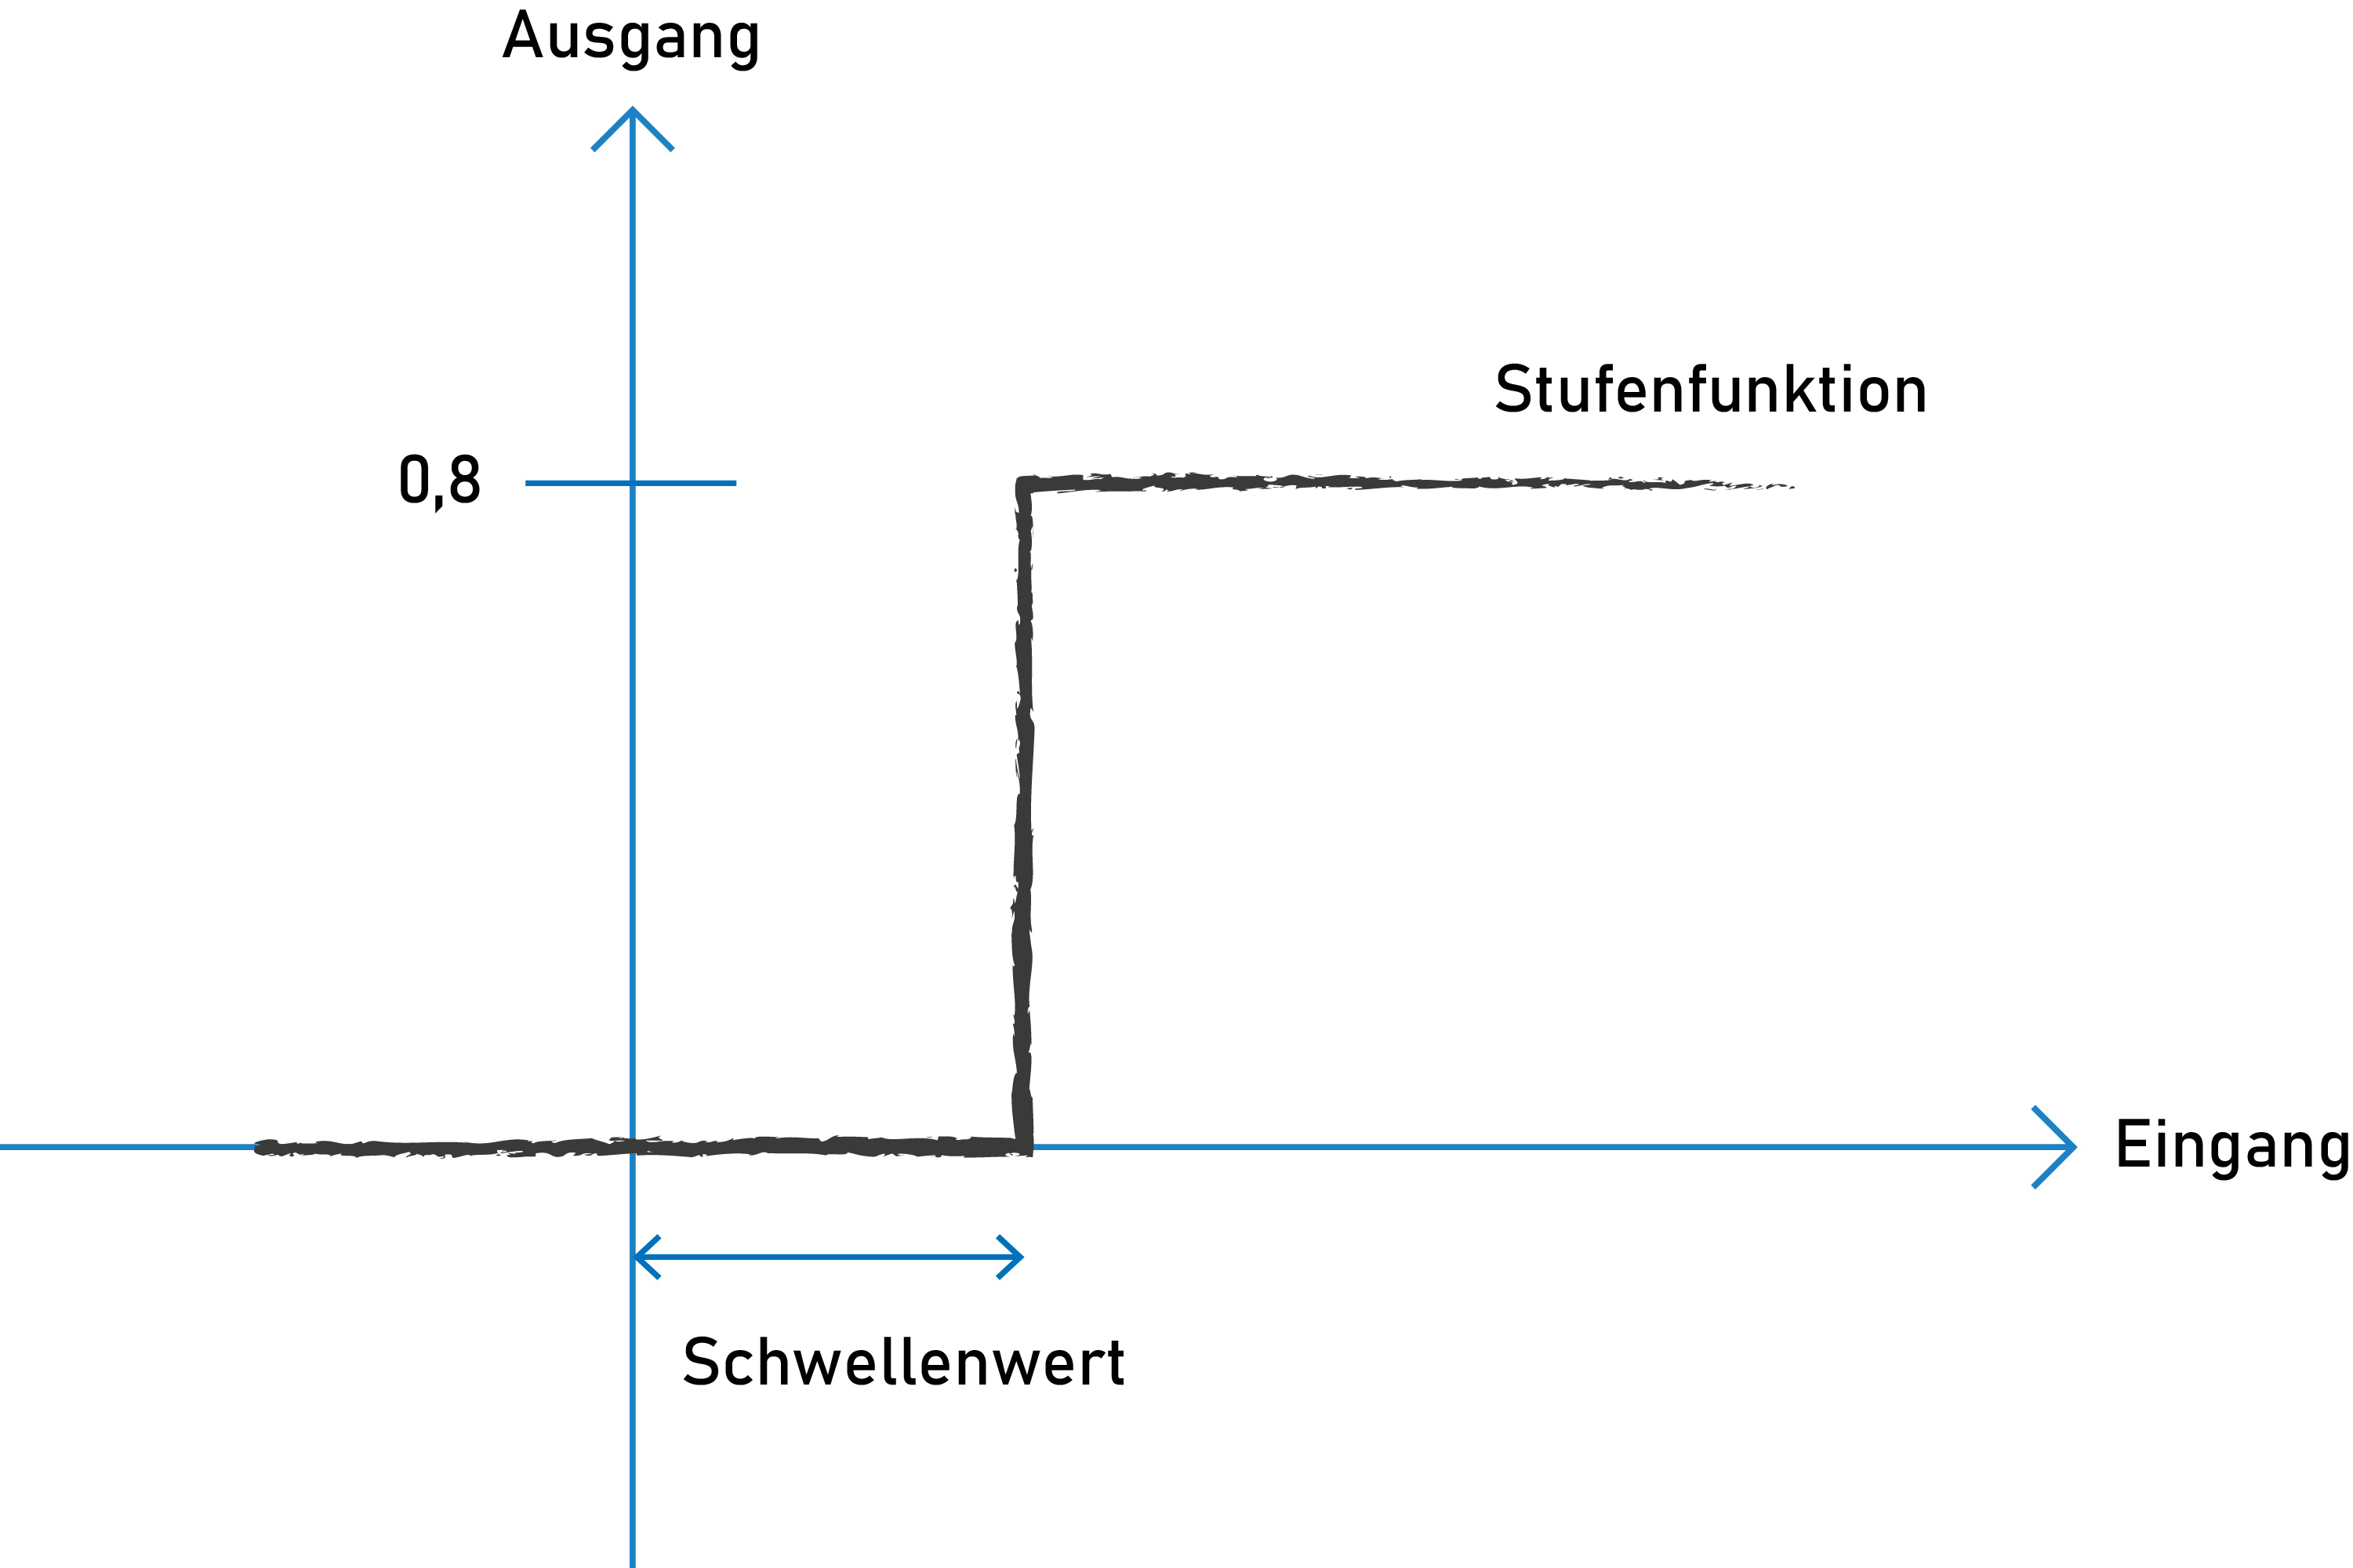
\includegraphics[width=9cm]{bilder/Stufenfunktion.jpg}
    \caption{Aktivierung eines Neurons mittels der Stufenfunktion.}
    \source{Philipp Benner in Anlehnung an \citet[33]{traiq_neuron}}
    \label{stufenfunktion}
\end{figure}

\subsubsection*{Weight} \citet[37]{traiq_neuron} erklärt, dass die uns bekannten Verbindungen zwischen den Neuronen einem sogenannten \textit{Weight} oder Gewicht unterliegen würden. Dies ist ein einfacher Multiplikator für den Ausgangswert eines Neurons. Beträgt etwa der Ausgangswert nach der Aktivierungsfunktion 0,8 und das Gewicht 0,5, so beläuft sich der neue Ausgangswert, der am Eingang des nächsten Neurons anliegt, auf 0,4.

\subsubsection*{Input Layer} Wie in Abbildung \ref{neuronalesnetz} zu sehen, besteht das Netz aus drei vertikalen Ebenen oder Layern. Der Input Layer stellt hierbei die erste Ebene dar. Um dem Netzwerk ein Bild zeigen zu können, werden aus den Pixeln des Bildes Input-Neuronen erzeugt, die jeweils den Helligkeitswert des Pixels annehmen. Beträgt die Auflösung des Bildes etwa 100 $\cdot$ 100 Pixel, so entstehen 10.000 Input-Neuronen. In \ref{neuronalesnetz} werden zur besseren Übersicht nur vier der 10.000 Input-Neuronen dargestellt. Alle Neuronen werden anschließend mit allen anderen Neuronen im darauffolgenden Hidden Layer verbunden. Auf die Eingabewerte wird keine Aktivierungsfunktion angewendet \parencite[S. 41]{traiq_neuron}.

\subsubsection*{Hidden Layer} Dieser stellt den zweiten Layer im Netz dar und enthält eine vom Programmierer vordefinierte Anzahl an Neuronen, die mit dem Input Layer verbunden sind. \citet[]{ramsundar-no-date} erklären, dass Layer, deren Neuronen mit allen Neuronen aus dem vorhergehenden Layer verbunden seien, die Bezeichnung \textit{Fully-connected-Layer} hätten. Es kann einen oder mehrere Hidden Layer geben, mit einer verschiedenen Anzahl an Neuronen \parencite[S. 52]{traiq_neuron}.

\subsubsection*{Output Layer} Dieser Layer stellt die Ausgabe des Netzes dar. Im Beispiel der Abbildung \ref{neuronalesnetz} laufen die Verbindungen des Hidden Layers in einem einzelnen Neuron im Output Layer zusammen und erzeugen eine letzte Ausgabe. Diese Ausgabe stellt die Sicherheit des Netzes als Wert von 0,0 bis 1,0 dar. Ein Output Layer kann aber auch mehr als nur ein Neuron haben. Mehr Neuronen als im Input Layer sind ebenso möglich \parencite[]{kukreja2016introduction}. \citet[36]{traiq_neuron} bezeichnet ein fertig aufgebautes Netz mit all seinen Layern und Funktionen als \textit{(engl.) Model}.


\section{Training eines neuronalen Netzes}
Im Folgenden wird das Training eines neuronalen Netzes vereinfacht erläutert. Damit das Netz nun lernt, die Bilder richtig zu klassifizieren, werden diesem verschiedene Bilder mit und ohne Hund gezeigt. Dazu wird ein ausgewogener Datensatz von Bildern mit und ohne Hund erstellt. Die Bilder erhalten ebenso ein Label mit \textit{0}, wenn kein Hund zu sehen ist, und mit \textit{1}, wenn das Bild einen Hund enthält. Anschließend, so führt der Autor fort, werde der Datensatz in \textit{Trainingsdaten} und \textit{Testdaten} unterteilt. Trainingsdaten werden zum Trainieren des Netzes verwendet, wohingegen die Testdaten erst nach dem Training zum Einsatz kommen. Somit lässt sich das Netz mit Daten testen, welches es noch nie zuvor gesehen hat, um genauere Aussagen über dessen Effizienz treffen zu können.\\

Laut \citet[302]{GoodBengCour16} würden den Gewichten des Netzes zufällige Werte aus einer Gauß-Verteilung zugewiesen werden, um ein effizientes Lernen zu ermöglichen. Mehrere Hidden Layer, die mit identischen Gewichten initialisiert werden, würden stets dasselbe lernen und somit könne sich das Netz nicht weiterentwickeln. Aber wie genau lernt nun ein neuronales Netz?\\

\citet[136]{traiq_neuron} erklärt, dass die Pixel der einzelnen Bilder in Input-Neuronen umzuwandeln seien, und die Helligkeitswerte dieser Pixel durch das Netz geschleust werden sollen. \citet[S. 42]{traiq_neuron} beschreibt, dass für jede Verbindung eines Neurons dessen Ausgabewert mit dem Gewicht der Verbindung multipliziert werde. Dieses Ergebnis pro Verbindung wird mit den anliegenden Verbindungen am Eingang eines Neurons summiert und in die Aktivierungsfunktion eingesetzt. Der neue Ausgabewert wird erneut mit dem Gewicht pro Verbindung multipliziert und der Kreislauf beginnt von vorn für den nächsten Layer im Netz. \citet[S. 44]{traiq_neuron} zufolge, würden komplexe Matrixmultiplikationen durchgeführt, um alle Verbindungen an allen Neuronen zu berechnen. Am Ende entsteht ein einziger Ausgangswert im Output Layer. Nun wird der Ausgangswert mit dem Label des Bildes verglichen. Falls das Bild eines Hundes am Netz angelegt wurde, sollte der Ausgangswert im besten Fall 1,0 betragen. Zu Beginn des Trainings wird das nicht der Fall sein, da das Netz noch nicht ausreichend lernen konnte. Nun muss der Fehlerwert, oder englisch \textit{Loss}, berechnen werden, den das Netz erzeugt hat.\\

Beispielsweise erzeugt das Netz für das Hundebild den Ausgabewert 0,3. Somit beträgt der Fehlerwert 0,7. Jetzt startet die sogenannte \textit{Backpropagation} oder etwa \textit{Fehlerrückführung}. \citet[S. 59]{traiq_neuron} erklärt, dass sie dazu genutzt werde, die Gewichte im Netzwerk zu verfeinern, um eine immer bessere Ausgabe mit geringerem Fehlerwert zu erzeugen. Anschließend beginne die Rückführung von hinten im Netz und es werde der Fehlerwert proportional zum Gewicht einer Verbindung aufgeteilt. Bei diesem Prozess werde der Fehlerwert kleiner, je weiter der Fehler zum Anfang des Netzes aufgeteilt werde. Anschließend wird jedes Gewicht so aktualisiert, sollte dasselbe Bild wieder durch das Netz geschleust werden, würde der Fehler geringer sein. \citet[21]{traiq_neuron} zufolge, sollen sich die Gewichte nur in geringem Maße verfeinern, da jedes Bild einen anderen Fehlerwert erzeuge. Dieses Maß würde über die sogenannte \textit{Learning Rate} geregelt. Die Verfeinerung der Gewichte und die Berechnung von komplexeren Fehlerwerten ist die Aufgabe des sogenannten \textit{Optimizers}, einem Algorithmus, der anhand einer mathematischen Funktion, das Minimum des Fehlerwertes für alle Gewichte im Netz sucht und es dahin gehend optimiert \parencite[]{doshi-2019}. Laut \citet[]{bushaev-2018} sei im Jahr 2014 ein Optimizer namens \textit{ADAM} veröffentlicht worden, der speziell für den Einsatz in Deep Neural Networks entworfen wurde. Ein Vorteil von ADAM sei, dass dieser adaptive Learning Rates benutze und somit individuelle Werte für die einzelnen Gewichte ermitteln konnte. Dies steigere die Performance des neuronalen Netzes. \\

Nach \citet[]{brownlee-2019} lasse sich das Training mit sogenannten \textit{Batches} verfeinern. Dabei werden nicht nach jedem Bild, welches durch das Netz geschleust wurde, die Gewichte aktualisiert, sondern erst nach einer gewissen Anzahl von Bildern. Mehrere Bilder seien Teil eines Batches, dessen Größe über die \textit{Batch Size} geregelt werde. Eine Batch Size von zehn enthält also zehn Bilder. Bei insgesamt 100 Bildern gibt es somit 10 Batches. Erst nachdem alle Bilder durch das Netz geschleust wurden und ein Fehlerwert für jedes Bild berechnet wurde, werden die Gewichte aktualisiert.\\

Nun wird dem Netz jeder Batch mit den dazugehörigen Labeln gezeigt, der Fehler berechnet und die Gewichte entsprechend aktualisiert. In der Praxis wiederholt sich dieser Durchlauf mehrmals in sogenannten Epochen. Bei zehn Epochen würde das Netz alle Bilder zehnmal sehen, was dem Optimizer erlaubt, die Effizienz des Netzes zu steigern \parencite[155]{traiq_neuron}.\\

Dies ist ein kleiner Teil an Mechanismen, die beim Training eines neuronalen Netzes ablaufen. Eine genauere Erläuterung passt jedoch nicht in den Rahmen dieser Arbeit. Daher soll ein Einblick in eine Art neuronaler Netze folgen, die auch als Teil dieser Forschung verwendet werden.

\section{Convolutional Neural Networks}
Sobald ein künstliches neuronales Netz für die Bildverarbeitung eingesetzt wird, bietet es sich an, anstatt Fully-connected-Layer mithilfe von \textit{Convolutional Layer} ein sogenanntes \textit{Convolutional-neural-Network} (CNN) zu schaffen. In diesen speziellen Layern wird ein Bild nicht mehr in eine Vielzahl an Neuronen zerlegt, sondern erhält seine ursprüngliche Form. \citet[135]{tariq_gan} erläutert, wenn das Bild das Netz durchlaufe, werde es mit einem Filter, dem sogenannten \textit{Kernel}, Pixel für Pixel gescannt. In Abbildung \ref{CNN} ist ein zweidimensionales Input Array zu sehen, das die Werte eines Pixelbildes darstellt. Dem Autor zufolge werde ein Kernel der Größe 3 $\cdot$ 3 erstellt und schrittweise über das Bild geschoben. Dabei würden die Werte im Input Array mit den Werten des Kernels multipliziert und anschließend alle entstehenden Produkte summiert werden. Dadurch entstehe ein Output Array einer geringeren Pixelanzahl mit den gefilterten Werten. Der Autor bezeichnet den Prozess des Verschiebens und das daraus resultierende Output Array als \textit{Faltung}.

\begin{figure}[ht]
    \centering
    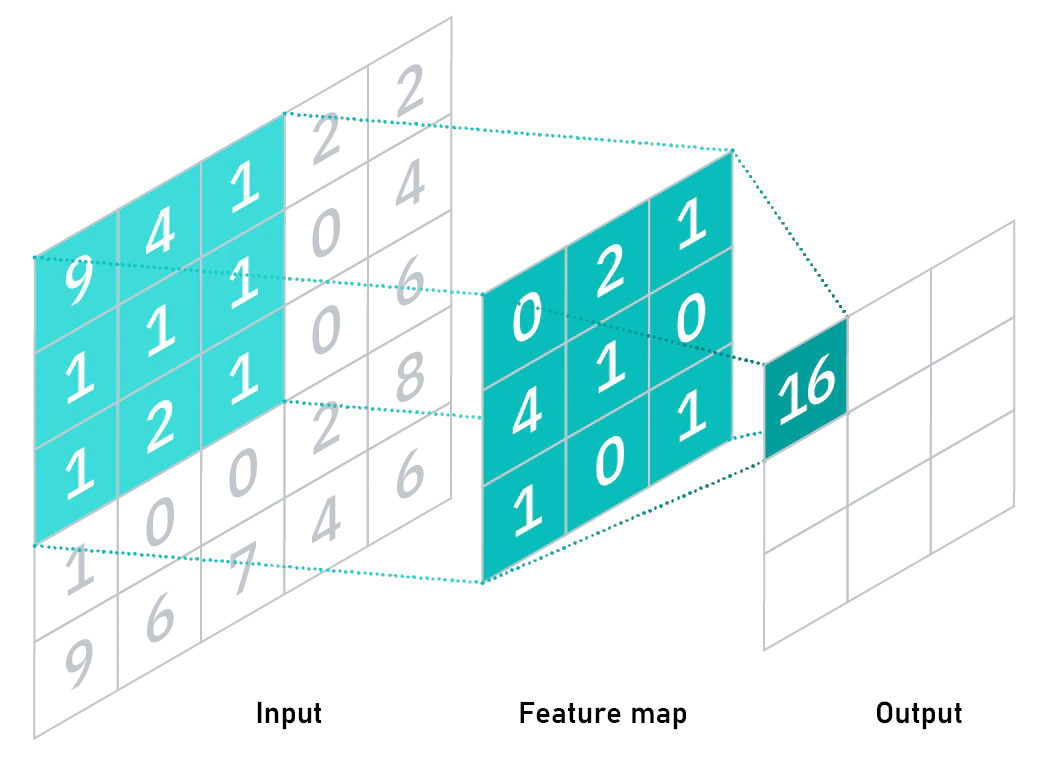
\includegraphics[width=9cm]{bilder/cnn.jpg}
    \caption{Arbeitsweise eines Convolutional Layer.}
    \source{Philipp Benner in Anlehnung an \citet{ibm-cloud-education-2021}}
    \label{CNN}
\end{figure}


\citet[133]{tariq_gan} zufolge werden die Werte im Kernel beim Training des Netzes verfeinert, damit eine sogenannte \textit{Feature Map} für bestimmte Merkmale im Bild entstehe. Diese Feature Maps seien laut \citet[]{brownlee-2019} auch die \textit{Channels} mit dem ein CNN arbeite. Ein RGB Bild habe für seine drei Farbkanäle die gleiche Anzahl an Input Channels im CNN. In den weiteren Convolutional Layern lassen sich die Größen für die Feature Maps/Channels aber nach Belieben erhöhen. Eine Feature Map lernt zum Beispiel, ob eine gewisse Pixelanordnung im Bild, etwa eine Linie oder ein Kreis zu sehen ist. Durch Kombination mehrerer Convolutional Layer lassen sich Merkmale auf einer höheren Ebene wie ein Auge oder eine Nase herausarbeiten. CNNs erreichen damit eine höhere Effizienz als herkömmliche Fully-connected-neural-Networks und benötigen weniger Speicher innerhalb der GPU \parencite[154]{tariq_gan}.

\section{Resiudal Neural Networks}
Je mehr Convolutional Layer ein neuronales Netz hat, desto wahrscheinlicher sei es laut \citet[]{nandepu-2021}, dass dieses Netz an den sogenannten \textit{Vanishing Gradients} leide. Dieses Phänomen handle von Layern am Anfang eines Netzes, die sich während des Trainings nicht mehr optimieren ließen, da der Fehler, der zu diesen Layern zurückgeführt würde, immer kleiner werde und irgendwann bei Null läge. Dann verschlechtere sich die Performance eines KI-Modells drastisch. Der Autor führt fort, dass sogenannte \textit{Residual Neural Networks} (RNN) eine Lösung für dieses Problem bieten würden. Dabei würden Abkürzungen in das Netz eingebaut werden, um den Weg der Backpropagation zu verkürzen. In Abbildung \ref{resnet} ist die schematische Darstellung eines sogenannten \textit{Residual Blocks} zu sehen. Der Autor erklärt, dass die eingehenden Daten durch zwei Verbindungen fließen würden. Diese würden durch die obere und untere Verbindung in Abbildung \ref{resnet} dargestellt. Die Blöcke der unteren Verbindung bestehen aus einem Convolutional Layer gefolgt von einem sogenannten \textit{Batch Normalization Layer} der die Input-Daten des Netzes neu berechnet und sie so formt, dass der Wertedurchschnitt der Daten bei null und die Varianz bei eins liegt \parencite[]{batchnorm}. \citet[]{nandepu-2021} führt fort, dass der Output des Batch Normalization Layers wird anschließend in die ReLU-Aktivierungsfunktion eingesetzt würde. Dieser Convolutional-Block wiederhole sich bis auf die Aktivierungsfunktion zweimal. Die Daten der oberen Verbindung würden ebenfalls durch einen Convolutional und Batch Normalization Layer fließen, jedoch komme hierbei nur ein einzelner Block zum Einsatz. Diese Verbindung werde auch als Abkürzung oder \textit{Shortcut} bezeichnet, da sie einige Layer überspringt. Am Ende des Residual Blocks würden die Daten aufsummiert werden und anschließend in den nächsten Layer im Netz fließen.

\begin{figure}[ht]
    \centering
    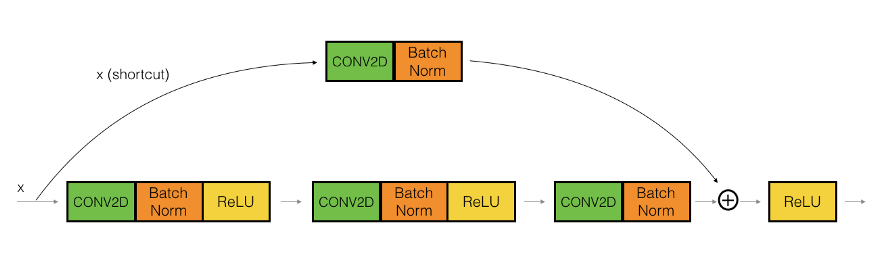
\includegraphics[width=14cm]{bilder/resnet.png}
    \caption{Aufbau eines Residual Blocks.}
    \source{\citet[]{iprathore-2020}}
    \label{resnet}
\end{figure}

Da die Daten, die durch das Netz fließen über die Shortcuts einen geringeren Weg zum ersten Layer während der Backpropagation haben, lassen sich Vanishing Gradients reduzieren und die Performance des KI-Modells aufrechterhalten.

\section{Generative Adversarial Networks}
Neuronale Netze werden nicht nur zur Klassifizierung eingesetzt, sondern sind auch in der Lage, neue Inhalte selbstständig zu erschaffen. \citet{Goodfellowgan} erforschten für diese Zwecke die sogenannten \textit{Generative Adversarial Networks} (GAN) oder \textit{Generativ gegnerische Netzwerke}. Gegnerisch deshalb, da bei diesem Konzept zwei künstliche Netzwerke gegeneinander antreten. Abbildung \ref{GAN} zeigt den Aufbau eines GANs, das handschriftliche Ziffern erzeugen soll. Ein Netzwerk ist ein sogenannter \textit{Diskriminator}, dieser entscheidet, ob sein Input echt oder künstlichen Ursprungs ist. Der Gegenspieler ist der \textit{Generator}, der Inhalte künstlich erzeugen kann. Schritt für Schritt versucht er seine Ergebnisse zu verbessern, um den Diskriminator später täuschen zu können, sodass die eigentlich künstlichen Ergebnisse als echt eingestuft werden.

\begin{figure}[ht]
    \centering
    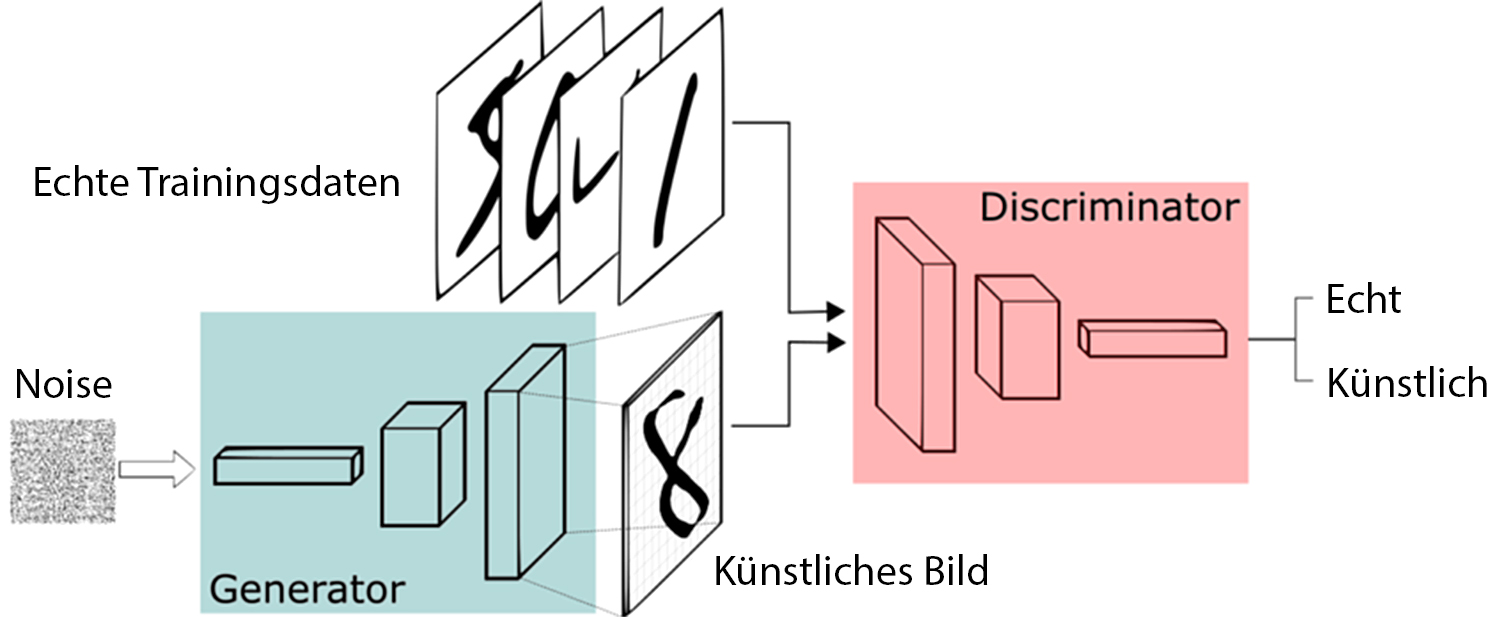
\includegraphics[width=11cm]{bilder/GAN_Net.jpg}
    \caption{Aufbau eines Generative Adversarial Networks.}
    \source{Philipp Benner in Anlehnung an \citet{silva-2020}}
    \label{GAN}
\end{figure}

Solche Netzwerke werden häufig für die Herstellung von statischen oder Bewegtbildern eingesetzt. Aber auch die Erstellung von 3D-Objekten oder Nutzung in Chatbots ist möglich \parencite[]{luber-2021}.

\section{Aufbau und Training eines Generative Adversarial Networks}
Generative Adversarial Networks, die zur Bildverarbeitung eingesetzt werden, basieren oftmals auf Convolutional Neural Networks um künstliche Bilder erzeugen. Im vorhergehenden Abschnitt wurden CNNs genutzt, um aus einem zweidimensionalen Pixelbild einen einzigen Ausgabewert zu erzeugen. Dafür wurden die Dimensionen und deren enthaltenen Werte schrittweise reduziert. \citet[61]{tariq_gan} erläutert, dass dieses Prinzip bei der Verwendung von GANs umgekehrt werde. Es ist möglich aus einer geringen Anzahl an ein- oder zweidimensionalen Werten, hochauflösende, mehrdimensionale Daten zu erschaffen. In Abbildung \ref{GAN} wird etwa ein zweidimensionales Pixelbild mit zufällig gewählten Werten, sogenanntes \textit{Noise}, an den Input des Generators angelegt. Das Bild hat die Auflösung 10 $\cdot$ 10 Pixel. Um die Auflösung des Bildes zu erweitern und den Noise in erkennbare Zahlen zu wandeln, kommen spezielle, umgekehrte Convolutional Layer zum Einsatz. \citet[145]{tariq_gan} erklärt, dass diese Erweiterung mit einer \textit{Transposed Convolution} oder \textit{transponierten Faltung} stattfinde. Dabei würden zusätzliche Pixel zwischen den bereits vorhandenen eingefügt, um ein größeres Bild zu erhalten. In Abbildung \ref{GAN} ist eine schematische Darstellung zu sehen, in der drei Transposed Convolutional Layer innerhalb des Generators die Auflösung eines Bildes erhöhen. 
Der Diskriminator nutzt hingegen normale Convolutional Layer, um Daten zu reduzieren und das Bild mit 0,0 für künstliche Bilder und 1,0 für echte Bilder zu klassifizieren. \\

Die Trainingsschleife wird im Folgenden nach \citet[65\psq]{tariq_gan} beschrieben. Im ersten Schritt wird dem Diskriminator ein echtes Trainingsbeispiel gezeigt und mitgeteilt, dass die Klassifizierung 1,0 betragen soll. Daraufhin wird dieser basierend auf dem Fehlerwert aktualisiert. Im zweiten Schritt wird dem Diskriminator eine künstliche Ausgabe des Generators gezeigt und mitgeteilt, dass die Klassifizierung 0,0 sei. Danach wird diese ebenfalls aktualisiert. Der Autor führt fort, dass im dritten Schritt dem Diskriminator erneut die Ausgabe des Generators gezeigt wird, diesmal wird aber dem Generator mitgeteilt, dass die Klassifizierung 1,0 betragen soll. Nun wird also nicht mehr der Diskriminator, sondern der Generator mit dem Fehlerwert aktualisiert und lernt somit, sich zu verbessern. Beide Netze sind zu Beginn schlecht im Generieren und Klassifizieren. Beide stehen im Wettbewerb gegeneinander und versuchen nach jeder Aktualisierung etwas besser zu werden. Im besten Fall hat der Generator nach genügend Trainingsepochen gelernt, visuell fehlerfreie, handschriftliche Ziffern zu erzeugen, die selbst von einem Menschen nicht mehr unterschieden werden können.

\section{Probleme und Fehlerquellen}
Es reicht nicht aus, einen Datensatz durch ein funktionierendes neuronales Netz zu schleusen und ein perfektes Ergebnis zu erwarten. Selbst nach etlichen Epochen und Tagen an Training kann es sein, dass ein Netz keine ausreichenden Ergebnisse liefert. Deshalb müssen neuronale Netze laufend auf verschiedene Arten optimiert werden. Im Folgenden sollen ein paar Probleme und Fehlerquellen erläutert werden.\\

\subsubsection*{Hardware Limitierung}
Laut \citet[]{fevbre-no-date} ließen sich Neuronale Netze schneller und effektiver auf einer GPU anstatt auf dem Prozessor trainieren. Dabei gäbe es die Limitierung, dass das Modell mit seinen Parametern vollständig in den Speicher der GPU passen müsse. Für kleine Modelle stelle dies kein Problem dar. Werden jedoch viele komplexe Ebenen wie Convolutional Layer hinzugefügt, würde die Speichergrenze schnell erreicht werden. Dieses Problem trat zum Beispiel während des Trainings des für diese Arbeit angefertigten Modells auf. Eine Möglichkeit ist es, die Layer im Modell zu reduzieren, was jedoch die Lernfähigkeit beeinträchtigt. Alternativ lassen sich die Modelle auf mehreren Grafikkarten parallel trainieren \parencite[]{giacaglia-2021}.

\subsubsection*{Black Box}
\citet[]{dickson-2019} erklärt, dass ein künstliches Neuronales Netz ein komplexes Geflecht aus selbst erlernten Parametern sei und es ließe sich schwierig vorhersagen, wie das Netz auf bestimmte Eingaben reagiere. Für triviale Aufgaben sei dies kein Problem, da solche Modelle jedoch zum Beispiel in medizinischen Diagnosen eingesetzt würden, sei eine hohe Zuverlässigkeit des Modells gefordert.

\subsubsection*{Unausgewogener Datensatz}
Die Qualität der Ausgabe eines Netzes hängt unter anderem sehr von den Daten ab, die dem Netz gezeigt werden. Dabei gilt es besonders darauf zu achten, diese Daten sorgfältig auszuwählen, damit der Datensatz keiner Verzerrung, dem sogenannten \textit{Bias} unterliegt. Als Beispiel sollten dem Diskriminator eines GANs während dem Training zur Zahlenerkennung, auch möglichst alle Zahlen gleichermaßen gezeigt werden. Würden ihm viele Zweier, aber nur wenig Neuner gezeigt werden, so könnte er diese nur schlecht erkennen \parencite[]{hao-2020}. Ebenso spielt die Qualität der Daten eine wichtige Rolle. Wird ein neuronales Netz zur Objekterkennung auf Bildern trainiert, sollten die Trainingsdaten beispielsweise nicht Abgeschnitten, verrauscht oder verschwommen sein \parencite[]{prov-international-inc-2022}.

\subsubsection*{Fehlende Balance}
\citet[67]{tariq_gan} zufolge sollen sich die im Wettbewerb gegeneinander stehenden Netze eines GANs stets in gleichem Maße verbessern. Eile der Diskriminator etwa dem Generator voraus, so schaffe es dieser nicht mehr aufzuholen. Sollte der Diskriminator zu langsam lernen, so verbessere der Generator seinen Output nicht und erzeuge unzureichende Ergebnisse.

\subsubsection*{Mode Collapse}
Ebenso zeigt \citet[95]{tariq_gan} das Phänomen des \textit{Mode Collapse}. Es tritt auf, wenn das Training eines GANs nicht ausbalanciert stattfindet. Der Generator konnte dem Diskriminator vorauseilen und erzeugt deshalb immer  dieselbe Ziffer, die anschließend als echt klassifiziert wird. Somit konnte dieser den Diskriminator austricksen, da der Generator zuvor kein brauchbares Feedback erhalten hat. Der Generator ist nun nicht mehr in der Lage, verschiedene Ausgaben zu erzeugen.

\subsubsection*{Overfitting} Es stelle laut \citet[]{baheti-2022} ein häufig auftretendes Problem beim Training künstlicher Intelligenzen dar. Das neuronale Netz schaffe es dabei nicht zu generalisieren und lerne die Trainingsdaten auswendig. Somit könne die Genauigkeit des Modells auf den Trainingsdaten sehr gut sein, würde es anschließend auf Daten getestet, die es zuvor noch nicht gesehen hat, nehme die Genauigkeit stark ab. \textit{Underfitting} dagegen bedeute, dass ein Modell selbst auf den Trainingsdaten keine ausreichende Genauigkeit erreiche. Um dieses Problem zu lösen, ließen sich die Komplexität des Modells variieren, der Datensatz erweitern oder sogenannte \textit{Dropout Layer} hinzufügen. Diese würden einige Verbindungen zwischen den Neuronen kappen und das Netz zwingen, besser zu generalisieren. \\

Mit den Grundlagen zu neuronalen Netzen und dem Wissen über Convolutional Neural Networks und GANs ist es nun möglich, den Aufbau des für diese Forschungsarbeit erstellten KI-Modells tiefergehend zu betrachten. Das KI-Modell besteht ebenfalls aus Convolutional und Residual Layern. Aus diesen werden ein Generator und Diskriminator erzeugt und trainiert. Das Ziel ist es zu evaluieren, ob ein neuronales Netz die Auflösung einer voxelbasierten Simulation bei gleichbleibender, visueller Qualität erhöhen kann.

%    \chapter{Stand der Forschung}
\thispagestyle{fancy}

Die Thematik der Deep Neural Networks im Simulationsbereich ist bereits weitläufig bekannt. Einige Forscher betreiben bereits Forschung in diesem Bereich und haben entsprechende Arbeiten publiziert. Da sich durchaus Parallelen zu der vorliegenden Arbeit auftun, sollen diese im Folgenden aufgezeigt werden. Vorgestellt werden drei wissenschaftliche Publikationen, welche Ergebnisse beim Upsamling von Rauchsimulationen mittels künstlicher Intelligenz erzielen konnten. Keine dieser Arbeiten nutzten die gleichen Methoden, die in dieser Arbeit verwendet werden. Auch wurde keines der Ergebnisse in einem VFX Umfeld bezüglich der visuellen Qualität und des Dateiformates OpenVDB getestet.\\

\citet[]{baidirectory} zeigen in \textit{Dynamic Upsampling of Smoke through Dictionary based Learning}, wie die Auflösung und Details von Rauchsimulationen mittels einer Bibliothek aus vortrainierten Mustern oder sogenannten \textit{Patches} verbessert werden kann. Das neuronale Netz lernt, wie es aus einer hochaufgelösten Rauchsimulation Patches extrahieren kann, die zur selben, niedrig aufgelösten Simulation passen. Es werden dafür paarweise die zusammengehörenden Patches niedriger und hoher Auflösung gespeichert. Wird dem Netz anschließend eine niedrig aufgelöste Simulation vorgelegt, findet es passende Patches mit hoher Auflösung aus der Bibliothek und erzeugt eine hochauflösende Ausgabe. Der Vorteil dieses KI-Modells ist, dass die Ausgabe der hochskalierten Daten einen hohen Detailreichtum innerhalb der Rauchsimulation aufweist. Ebenfalls wird nur ein Density Field benötigt, um eine Ausgabe zu erzeugen. Der Nachteil dieses KI-Modells ist hingegen, dass visuelle Artefakte innerhalb der Ausgabe auftreten können. Sollte das Netz Eingaben skalieren müssen, zu denen keine passenden Patches in der zuvor trainierten Bibliothek existieren, werden Artefakte in diesen Bereichen sichtbar.\\

Laut \citet[]{Gao_2021} sei es möglich, ein solches Upsampling mittels neuronaler Netze auch ohne hochauflösende Trainingsdaten zu schaffen. Dies zeigen die Autoren in \textit{Super-resolution and denoising of fluid flow using physics-informed convolutional neural networks without high-resolution labels}. Während des Trainings bestehen die Inputs nur aus niedrig aufgelösten Datensätzen. Um das Netz zu verfeinern, wird analysiert, wie ähnlich der Output des Netzes an einer physikalisch korrekten Berechnung der Strömung ist. Die Autoren nannten dies \textit{Physics-informed training}. Der Vorteil dieses Netzes besteht darin, dass es nicht mit zwei Datensätzen, bestehend aus niedrig und hochaufgelösten Daten, trainiert werden muss und trotzdem in der Lage ist, eine hochauflösende Ausgabe zu erzeugen. Der Nachteil dieses KI-Modells sind die fehlenden Erkenntnisse im dreidimensionalen Raum, da das Netz nur mit zweidimensionalen Daten trainiert wurde. \\

Die Autoren der Publikation \textit{tempoGAN: A Temporally Coherent, Volumetric GAN for Super-resolution Fluid Flow \parencite{xie2018tempoGAN}}, trainierten ein GAN, welches es ermöglicht, ein Upsampling auf Basis des Density und Velocity Fields einer Rauchsimulaition zu erzeugen. Das Modell lernt mit niedrig aufgelösten Daten, die physikalische Beziehung zwischen Density und Velocity zu verstehen. Der Generator erzeugt, basierend auf einem niedrig aufgelösten Input, einen hochaufgelösten Output. Dabei gelang den Autoren, eine visuell artefaktfreie Qualität über mehrere Frames hinweg zu garantieren. Dies erreichten sie, indem der Generator mit drei aufeinanderfolgenden Frames trainiert wurde und somit eine temporale Kohärenz lernte. Dies stellt einen großen Vorteil des KI-Modells dar und ist im VFX-Bereich besonders wichtig. Der Nachteil dieses KI-Modells ist jedoch, dass es nicht in der Lage ist, mit Simulationsdaten aus Houdini oder anderen Programmen der VFX-Industrie zu arbeiten. Ebenfalls bedarf die Speicherung des Velocity Fields einer Simulation im Vergleich zum Density Field mehr Speicherplatz. Da der Betrieb von Servern zum Speichern der Daten einen hohen Kostenaufwand mit sich bringt, bietet sich hier die Grundlage zur Forschung, ob das Velocity Field mit dem Temperature Field einer Simulation für das Training des KI-Modells ausgetauscht werden kann. \\

Zusammenfassend lässt sich feststellen, dass keines der genannten KI-Modelle in einem VFX-Umfeld genutzt werden könnte, da sie nicht mit dreidimensionalen Daten oder dem Dateiformat OpenVDB arbeiten. Dies zeigt, dass hier ein deutlicher Bedarf an Forschung besteht und die vorliegende Arbeit das Potenzial hat, diese Lücke zu schließen.


%    \chapter{Methodik}
\thispagestyle{fancy}

\section{Art der Methodik}
Als Forschungsgrundlage dieser Arbeit sollte ein Experiment dienen, das den qualitativen Anspruch erhob, neue Erkenntnisse im Bereich der Forschungsfrage zu schaffen. Ein Experiment stellte hierfür die geeignetste Form dar, da die Ergebnisse direkt im VFX-Kontext evaluiert werden konnten. Die allgemeine Vorgehensweise und Wahl der Gütekriterien wird im Folgenden beschrieben.

\section{Aufbau und Ablauf des Experiments}
Um die Objektivität und Reliabilität der Forschungsarbeit zu wahren, wurden standardisierte Verfahren zur Datenerhebung implementiert. Die Erzeugung und Speicherung der 3D-Daten fand stets auf dieselbe Weise in der Simulationssoftware statt. Um die Simulationsdaten anschließend in eine für die künstliche Intelligenz passende Form zu bringen, kamen eigens angefertigten Skripte der Programmiersprache Python \parencite[]{python} zum Einsatz. \\

Der Versuchsaufbau bestand aus der Erzeugung eines Datensatzes von Rauchsimulationen in der Software Houdini. Es wurden 72 individuelle Simulationen erstellt, die jeweils aus 80 kohärenten Frames bestehen. In jeder Simulation wurde Rauch aus entweder einem oder drei kugelförmigen Emittern erzeugt und stieg nach oben. Die Density des Rauches dissipierte über eine pro Simulation zufällig gewählte Zeit und ebenso wirkten Kräfte wie Wind und Turbulenzen auf die Simulation, deren Richtung und Amplitude variierte. Diese Varianzen waren stets gleich für die Erzeugung einer einzelnen Simulation, sie unterschieden sich nur zu anderen Simulationen. Die maximale Voxelanzahl pro Dimension betrug 200 Voxel und fand somit in einem Container, der sogenannten \textit{Bounding Box}, mit der Maximalgröße 208 $\cdot$ 208 $\cdot$ 208 Voxel statt. Die Differenz von 8 Voxeln ergab sich durch interne Verfahren im OpenVDB Format, sie wurden jedoch in der fortlaufenden Bearbeitung der Daten entfernt. Die gespeicherte OpenVDB Datei eines Frames enthielt das Density und Temperature Field der Simulation.\\

Da eine OpenVDB Datei nicht direkt als Input für ein neuronales Netz genutzt werden konnte, fand eine Konvertierung aller Frames in ein 3D-NumPy-Array statt. Die Programmbibliothek \textit{NumPy} \parencite[]{harris2020array} diente im Allgemeinen zur Bearbeitung von Arrays in Python. Diese Konvertierung erfolgte mit dem Python-Modul des OpenVDB Herstellers. Das neuronale Netz wurde im Python Framework \textit{PyTorch} \parencite[]{torch} erstellt. Die Aufgabe des Netzes sollte sein, die Auflösung jeder Dimension einer Input-Simulation auf die vierfache Größe skalieren. Zur Evaluation des Trainings diente der ausgegebene Fehlerwert des Netzes. Zur visuellen Überprüfung der Ausgabe diente eine OpenVDB Datei pro Frame. Der genaue Aufbau dieses Netzes folgt im nächsten Abschnitt. \\

Nach dem Training sollte ein Python-Skript das Modell der künstlichen Intelligenz nutzen, um eine beim Training nicht verwendete Simulation zu skalieren. Dazu wurde eine neue Simulation erzeugt und im OpenVDB Format gespeichert. Das Python-Skript erhielt den Speicherort der Simulation-Frames und konvertierte jeden Frame zu einem dreidimensionalen NumPy-Array. Anschließend wurde eine Low Resolution, oder niedrig aufgelöste Version des Arrays erstellt und durch das Netz hochskaliert, um die ursprüngliche Auflösung zu erhalten. Diese in der Auflösung skalierte Version stellte die Grundlage für die Evaluation der Gütekriterien dar. \\

Ebenso wurden bereits vorhandene Rauchsimulationen erfasst, um Aussagen über die Simulationszeit und Speichergröße treffen zu können. Dazu wurden 28.950 OpenVDB Files eines Projektes von Mackevision untersucht. Jede Datei enthielt folgende Werte: 

\begin{center}
\begin{tabular}{ l l }

$\bullet$ Dateispeicherort & $\bullet$ Voxel-Anzahl \\
$\bullet$ Dateigröße & $\bullet$ Containergröße der Simulation \\
$\bullet$ Erstellungsdatum der Datei & $\bullet$ Frameindex in der Simulation \\
$\bullet$ Simulation Fields & $\bullet$ Frameindex in Prozent \\

\end{tabular}
\end{center}


\section{Gütekriterien}
Um festzustellen, ob der Einsatz eines neuronalen Netzes zum Upsampling von Rauchsimulationen ein optimales Ergebnis erzielt, sollte dieser anhand folgender Kriterien evaluiert werden.\\

\subsubsection*{Artefaktfreiheit} Die Ausgabe des Netzes sollte keine spatialen visuellen Artefakte in die Simulation einführen. Das galt ebenso für die temporale Kohärenz der einzelnen, aufeinanderfolgenden Frames.\\

\subsubsection*{Formgleichheit} Die generelle Form der ursprünglichen, niedrig aufgelösten Simulation sollte erhalten bleiben. Es sollten jedoch mehr Details im Rauch sichtbar sein.\\

\subsubsection*{Schnelligkeit} Das Upsampling durch das neuronale Netz sollte für alle Frames einer Simulation weniger Zeit in Anspruch nehmen, als das Simulieren derselben Simulation in vierfacher Größe ihrer Auflösung pro Dimension. \\

\subsubsection*{Datensparsamkeit} Das neuronale Netz soll das Upsampling nur mit dem Density und Temperature Field einer Simulation durchführen können.\\


%    \chapter{Implementierung}
\thispagestyle{fancy}

Als Basis der Implementierung diente das tempoGAN nach \citet{xie2018tempoGAN}. Der Unterschied zu dem tempoGAN KI-Modell bestand in der Wahl der Fields, die diese Arbeit für das Training nutze. Anstatt das Velocity Field zu nutzen, kam das Temperature Field zum Einsatz. Dieses hat ebenso wie das Velocity Field eine physikalische Grundlage innerhalb der Simulation, benötigte jedoch weniger Speicherplatz. Ebenso waren beide neuronalen Netze mit weniger Convolutional Layer aufgebaut. Diese und weitere Unterschiede zu tempoGAN werden in den folgenden Abschnitten näher betrachtet.

\section{Setup}
Das Experiment wurde auf einer von Mackevision zur Verfügung gestellten Workstation durchgeführt. Sie bestand unter anderem aus dem Intel Prozessor E5-2630 mit sechs Kernen, der Grundtaktfrequenz 2,30 GHz und einer einzelnen NVIDIA RTX 3060 Ti mit 8 Gigabyte VRAM. Die Speicherung der Daten erfolgte auf dem firmeninternen Server. Als Betriebssystem diente Windows 10.


\section{Datenerhebung}
Ein grundsätzlicher Unterschied zur tempoGAN-Implementierung war die Erzeugung des Datensatzes von Simulationsdaten. Dort wurden die Simulationen innerhalb der Software \textit{Mantaflow} \parencite{mantaflow} erstellt. Ebenso setzt Mantaflow auf ein selbst entwickeltes Dateiformat der Endung \textit{.uni}, um Raster- und Partikeldaten zu speichern \parencite[]{thuerey-group-no-date}. Houdini hingegen arbeitet nicht mit einer Mantaflow-Implementierung und um zu testen, ob ein KI-Modell mit den Daten der gängigen Programme im VFX Bereich trainiert werden konnte, wurde auf die Nutzung von Mantaflow verzichtet. 
Als Trainingsdaten dienten die wie im Methodik-Abschnitt erzeugten Rauchsimulationen verwendet. Hier lag ein weiterer Unterschied zur tempoGAN-Implementierung. Die Forscher trainierten das KI-Modell mit den Density und Velocity Fields ihrer Simulationen. Wurde jedoch auf den Export des Velocity Fields verzichtet und stattdessen das Temperature Field genutzt, ließen sich durchschnittlich 68\% Speicherplatz sparen (vgl. Tabelle \ref{tab:veltemp}). Für diesen Speichervergleich wurden jeweils drei Varianten einer Simulation erzeugt und gespeichert. Pro Variante wirkten unterschiedliche Kräfte. Für jede Variante wurden jeweils die Felder Density + Velocity und Density + Temperature im OpenVDB Format gespeichert. Die reduzierte Dateigröße war der Grund, das Velocity Field mit dem Temperature Field für das Experiment dieser Arbeit auszutauschen.

\begin{table}[ht]
    \centering
    \caption{Speicherplatzbedarf in GB einer Simulation mit jeweils 50 Frames.}
    \begin{tabular}{|r|c|c|}
        \hline
         & Density + Velocity [GB] & Density + Temperature [GB]  \\
         \hline
         Variante 1 & 2,17 & 0,955 \\
         Variante 2 & 2,48 & 0,632 \\         
         Variante 3 & 0,447 & 0,08 \\
         \hline
        \hline
         $\varnothing$  & 1,70 & 0,55 \\
         \hline
    \end{tabular}
    
    \label{tab:veltemp}
\end{table}

Das Dateiformat OpenVDB speichert für jeden Frame nur die aktiven Voxel einer Simulation und nicht alle Voxel der maximalen Bounding Box. Zu Beginn der Simulation sind kaum aktive Voxel vorhanden, was eine geringe räumliche Größe der Simulation bedeutet. So entsteht eine Datei mit wenig Voxeln und einer kleineren Bounding Box. Da ein neuronales Netz eine unveränderliche Anzahl an Input-Neuronen hat, darf die Anzahl an Voxeln, die an den Inputs angelegt wird, nicht variabel sein. Es müssen für jeden Frame immer gleich viele Werte an die Inputs angelegt werden. Dazu wurden aus der OpenVDB Datei eines Frames die Density und Temperature Fields jeweils in 3D-NumPy-Arrays konvertiert. Ein Python-Skript erstellte für jedes Field ein zweites Array pro Frame, dessen Auflösung 192 $\cdot$ 192 $\cdot$ 192 betrug. Diese Auflösung wurde gewählt, da sie ein Vielfaches von 64, einer genutzten Größe im KI-Modell und eine Annäherung an die ursprüngliche Größe des OpenVDB Frames ist. Alle Werte dieses Arrays bestanden aus dem Wert null. Anschließend wurde das aus dem OpenVDB Frame erzeugte Array in das mit Null-Werten initialisierte kopiert, um ein neues Array zu erhalten, dessen Auflösung immer gleich war, dafür mit unterschiedlichen Werten für Density und Temperature. Das Python-Skript kombinierte die beiden neuen 3D-NumPy-Arrays anschließend wieder zu einem einzigen NumPy File. Somit wurde aus jedem Simulationsframe immer die gleiche Anzahl an Input-Neuronen erzeugt, auch wenn diese zu Beginn einer Simulation aus vielen Null-Werten bestanden.


\section{Aufbau des Netzes}
Die Architektur des neuronalen Netzes unterschied sich ebenso zu der tempoGAN-Implementierung. Das tempoGAN-Netz besteht aus zwei Diskriminatoren und einem Generator (Abbildung \ref{tempoGAN-Aufbau}). Laut \citet[]{xie2018tempoGAN} sei das Netz mit hochaufgelösten Simulationen ($Y$) und heruntergerechneten, niedrig aufgelösten Versionen derselben Simulation ($X$) trainiert worden. Ebenso sei Diskriminator $D_S$ dafür zuständig, spatiale Aspekte zu erkennen und zu klassifizieren, ob dessen Input echt sei. Die Autoren führten fort, dass Diskriminator $D_t$ sich auf temporale Aspekte fokussiere, indem er drei temporal kohärente Frames als Input bekomme und sie auf Echtheit klassifiziere. Der Generator erhalte ebenso drei kohärente niedrig aufgelöste Frames aus Density und Velocity Daten und erzeuge aus diesen einen Output für die Diskriminatoren. In der Trainingsschleife würden die Diskriminatoren dem Generator stetig Feedback geben, um sich zu verbessern. 

\begin{figure}[ht]
    \centering
    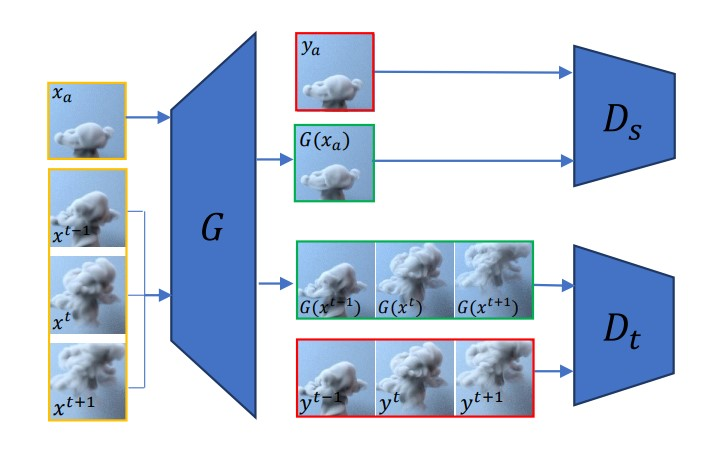
\includegraphics[width=11cm]{bilder/tempoGAN.jpg}
    \caption{Schematischer Aufbau des tempoGAN.}
    \source{\citet[95:2]{xie2018tempoGAN}}
    \label{tempoGAN-Aufbau}
\end{figure}

Das Netz dieser Arbeit hingegen nutzte jeweils nur einen Generator und Diskriminator während des Trainings. Ebenfalls wurden der Generator und Diskriminator jeweils mit einem Batch von 3D-Arrays trainiert. Ein Batch bestand aus mehreren Datenpaketen und jedes Paket erhielt drei temporal kohärente Frames einer Simulation. Jeder Frame, bestehend aus einem 3D-Array und wurde nochmals in kleinere, im Folgenden \textit{3D-Sub-Arrays} genannt, unterteilt. So hatte das ursprüngliche 3D-Array beispielsweise eine Auflösung von 192 $\cdot$ 192 $\cdot$ 192 Voxel und wurde anschließend in 27 kleinere 3D-Sub-Arrays mit der Auflösung 64 $\cdot$ 64 $\cdot$ 64 Voxel unterteilt. Das Training des Diskriminators bestand aus einem Batch mit zehn solcher 3D-Sub-Arrays. Anfängliche Tests zeigten, dass eine 1:1 Abbildung des tempoGAN-Netzes zu viel Speicherplatz innerhalb der Grafikkarte benötigte, weshalb es nicht möglich war, alle 27 3D-Sub-Arrays für das Training zu nutzen. Für den Generator wurden Low-Resolution-Versionen der 3D-Sub-Arrays erstellt. Die Auflösung dieser im Folgenden genannten \textit{LowRes-3D-Arrays} betrug 16 $\cdot$ 16 $\cdot$ 16 Voxel und wurde auf 64 $\cdot$ 64 $\cdot$ 64 Voxel hochskaliert, um die ursprüngliche Auflösung für den Input des Diskriminators zu erzeugen. Die tempoGAN-Implementierung nutzte hingegen alle 3D-Sub-Arrays eines Frames. Ebenso wurden weniger Convolutional und Residual Layer als im tempoGAN eingesetzt. Der Grund hierfür war, dass nur somit ein Training auf der Grafikkarte durchgeführt werden konnte. Deshalb wurde eine funktionierende Minimalvariante erstellt und trainiert. Im Folgenden werden die Architekturen des Generators und Diskriminators genauer beschrieben.

\subsection{Generator}
Es wurde eine höhere Anzahl an Convolutional und Residual Layer für den Generator, als für den Diskriminator gewählt, da dieser die komplexere Aufgabe des Upsamplings übernimmt. Die Architektur des Generators bestand aus einem anfänglichen Upsampling der Input-Daten und zwei lernfähigen Residual Blöcken. Die Upsampling Layer skalierten die Input-Daten auf die gewünschte Output-Größe. Es wurden ähnlich einer Transposed Convolution neue Voxel zwischen den bereits vorhandenen eingefügt. Diese neuen Voxel erhielten, basierend auf der \textit{Nearest Neighbor Interpolation}, denselben Wert, wie die am nächsten zu ihnen stehenden Nachbarn \parencite[]{nearestneighbor}. Anschließend wurden die Daten parallel durch die Residual Shortcut 1 und den Convolutional Block 1 geschleust. Letzterer enthielt doppelt so viele Convolutional Layer und erzeugte ebenso mehr Output Channels. Somit konnte das Netz mehr Feature Maps lernen und im besten Fall einen höheren Detailgrad in der Ausgabe erzeugen. Nachdem die Daten durch die beiden Blöcke geschleust wurden, konnten ihre Outputs summiert werden und dienten als Input für den nächsten Residual Block. Dort wurden die Daten wieder parallel in den die Residual Shortcut 2 und den Convolutional Block 2 gegeben und ihr Output anschließend summiert. Die Verfeinerung der Gewichte übernahm der ADAM Optimizer mit einer Lernrate von 0.0001. Es folgt eine grobe Übersicht über den Aufbau des Generators. Eine ausführliche Version findet sich im Anhang.
\newpage

\begin{enumerate}
    \item \underline{Input:} LowRes-3D-Array der Größe 16 $\cdot$ 16 $\cdot$ 16 Voxel mit 2 Input Channels (Density und Temperature)
    \item \underline{Upsample:} Ein Upsampling der 3D-Input-Daten zur Größe 32 $\cdot$ 32 $\cdot$ 32 Voxel.
    \item \underline{Upsample:} Ein Upsampling zur Größe 64 $\cdot$ 64 $\cdot$ 64 Voxel
    \item \underline{\textbf{Residual Block 1}} 
    \item[] \underline{Residual Shortcut 1} 
        \begin{enumerate}
            \item \underline{3D Convolutional Layer:} Input Channels 2, Output Channels 4
            \item \underline{3D BatchNorm:} Formt den Batch so, dass sein Durchschnittswert bei null und die Varianz bei eins liegt. Gilt für alle folgenden BatchNorm Layer.
        \end{enumerate}

    \item[] \underline{Convolutional Block 1}
        \begin{enumerate}
            \item \underline{3D Convolutional Layer:} Input Channels 2, Output Channels 4
            \item \underline{3D BatchNorm:}
            \item \underline{ReLU Aktivierungsfunktion:}
            \item \underline{3D Convolutional Layer:} Input Channels 2, Output Channels 4
            \item \underline{3D BatchNorm:}
        \end{enumerate}
        
    \item \underline{Summierter Output aus Residual-Shortcut 1 und Convolutional Block 1}
    \item \underline{\textbf{Residual Block 2}} 
    \item[] \underline{Residual Shortcut 2} 
        \begin{enumerate}
            \item \underline{3D Convolutional Layer:} Input Channels 4, Output Channels 2
            \item \underline{3D BatchNorm:}
        \end{enumerate}
    \item[] \underline{Convolutional Block 2}
        \begin{enumerate}
            \item \underline{3D Convolutional Layer:} Input Channels 4, Output Channels 8
            \item \underline{3D BatchNorm:}
            \item \underline{ReLU Aktivierungsfunktion:}
            \item \underline{3D Convolutional Layer:} Input Channels 8, Output Channels 2
            \item \underline{3D BatchNorm:}
        \end{enumerate}
    \item \underline{Summierter Output aus Residual Shortcut 2 und Convolutional Block 2}
    \item \underline{Output} 3D-Sub-Array der Größe 64 $\cdot$ 64 $\cdot$ 64 Voxel mit 2 Channels
\end{enumerate}

\subsection{Diskriminator}
Es folgt eine grobe Übersicht der Architektur des Diskriminators. Dieser wurde so aufgebaut, dass er dem temporalen Diskriminator der tempoGAN-Implementierung ähnelt. Als Input-Daten erhielt der Generator sechs Input Channels. Sie bestanden aus dem Density und Temperature Field eines Simulation-Frames. Insgesamt wurden drei aufeinanderfolgende Frames einer Simulation an den Input angelegt, um auf sechs Input Channels zu kommen. Jeder Channel bestand aus einem 3D-Sub-Array der Auflösung 64 $\cdot$ 64 $\cdot$ 64 Voxel. Über mehrere Convolutional Layer, einem Fully-Connected-Layer und einem einzelnen Output-Neuron lernte der Diskriminator den Input zu klassifizieren. Seine Ausgabe betrug 0,0, wenn er sich sicher war, dass die Input-Daten künstlich sind und 1,0, wenn er sie als echt klassifizierte. Zur Verfeinerung der Gewichte wurde ebenfalls der ADAM Optimizer mit einer Lernrate von 0.0001 eingesetzt. Eine ausführliche Version der Architektur findet sich ebenfalls im Anhang.

\begin{enumerate}
    \item \underline{Input} 3D-Sub-Array der Größe 64 $\cdot$ 64 $\cdot$ 64 Voxel mit 6 Input Channels (Density+Temperature für 3 Simulation-Frames)
    \item \underline{3D Convolutional Layer} Input Channels 6, Output Channels 8
    \item \underline{3D BatchNorm}
    \item \underline{Leaky-ReLU Aktivierungsfunktion} Eine Variante der normalen ReLU-Funktion, schneidet Werte im Minusbereich nicht ab \parencite[]{liu-2019}.
    \item \underline{3D Convolutional Layer} Input Channels 8, Output Channels 16
    \item \underline{3D BatchNorm}
    \item \underline{Leaky-ReLU Aktivierungsfunktion}
    \item \underline{3D Convolutional Layer} Input Channels 16, Output Channels 1
    \item \underline{Flatten} Wandelt alle dreidimensionalen Werte in einen eindimensionalen Layer an Neuronen um \parencite[]{meta-aiflatten}.
    \item \underline{Fully-Connected-Layer} Verbindet den eindimensionalen Layer an Neuronen mit dem letzten Neuron.
    \item \underline{Sigmoid-Aktivierungsfunktion} Erzeugt eine Ausgabe zwischen 0,0 und 1,0 \parencite[]{wood-2020}.
    \end{enumerate}


\section{Training des Netzes}
Im Folgenden wird die Trainingsschleife der beiden Netze erläutert. Die Daten entstammten dem in der Methodik beschriebenen Datensatz. Innerhalb einer Epoche wurden somit 5760 Frame-Pakete, zu sehen in Abbildung \ref{paket}, bestehend aus drei temporal kohärenten Frames mit Density und Temperature Fields verwendet. \\

\begin{figure}[ht]
    \centering
    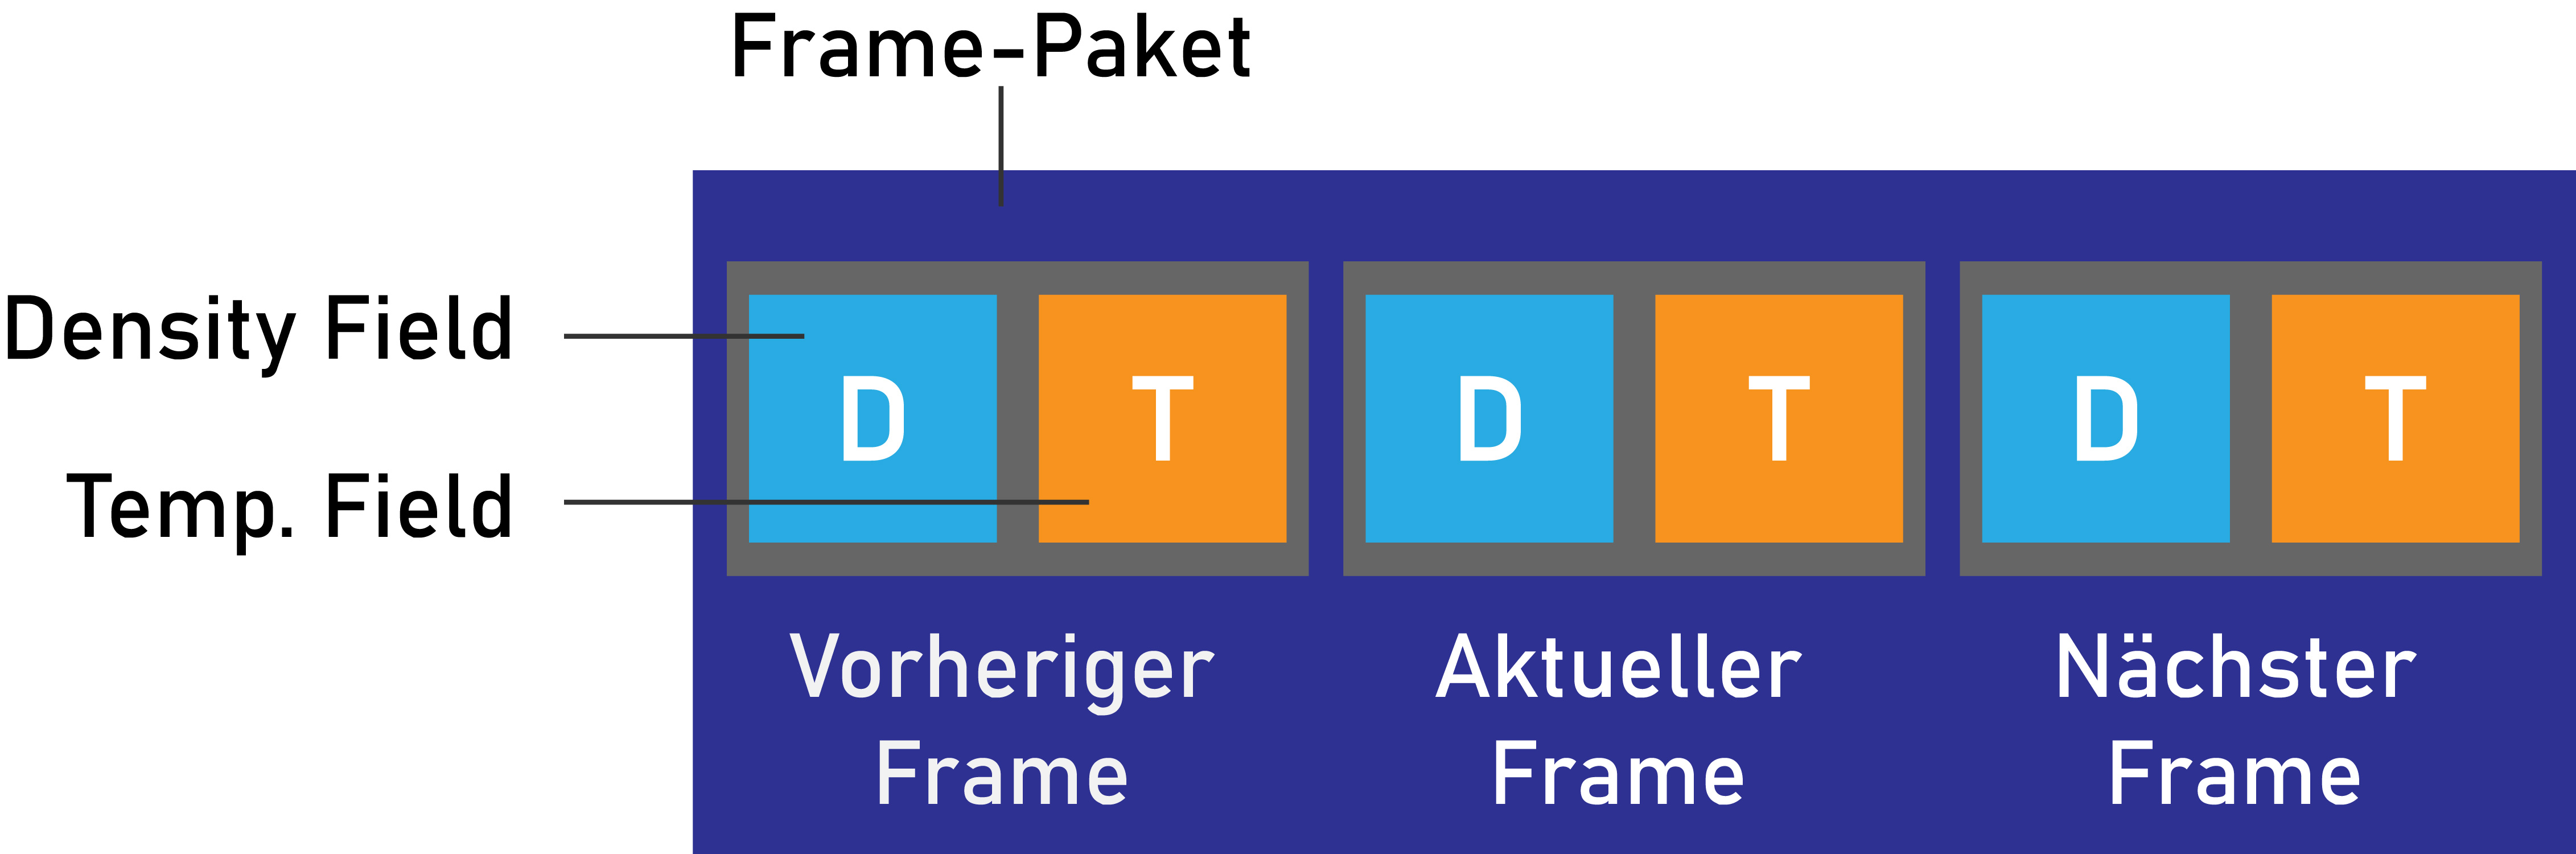
\includegraphics[width=11cm]{bilder/framepaket.jpg}
    \caption{Der Aufbau eines Frame-Pakets.}
    \source{Philipp Benner}
    \label{paket}
\end{figure}

Ein Batch enthielt zehn Frame-Pakete bestehend aus den Density und Temperature Fields des vorherigen, aktuellen und nächsten Frames. Jedes Field der Ursprungsgröße 192 $\cdot$ 192 $\cdot$ 192 Voxel wurde in 27 3D-Sub-Arrays der Größe 64 $\cdot$ 64 $\cdot$ 64 Voxel zerlegt (Abbildung \ref{fieldarray}). \\


\begin{figure}[ht]
    \centering
    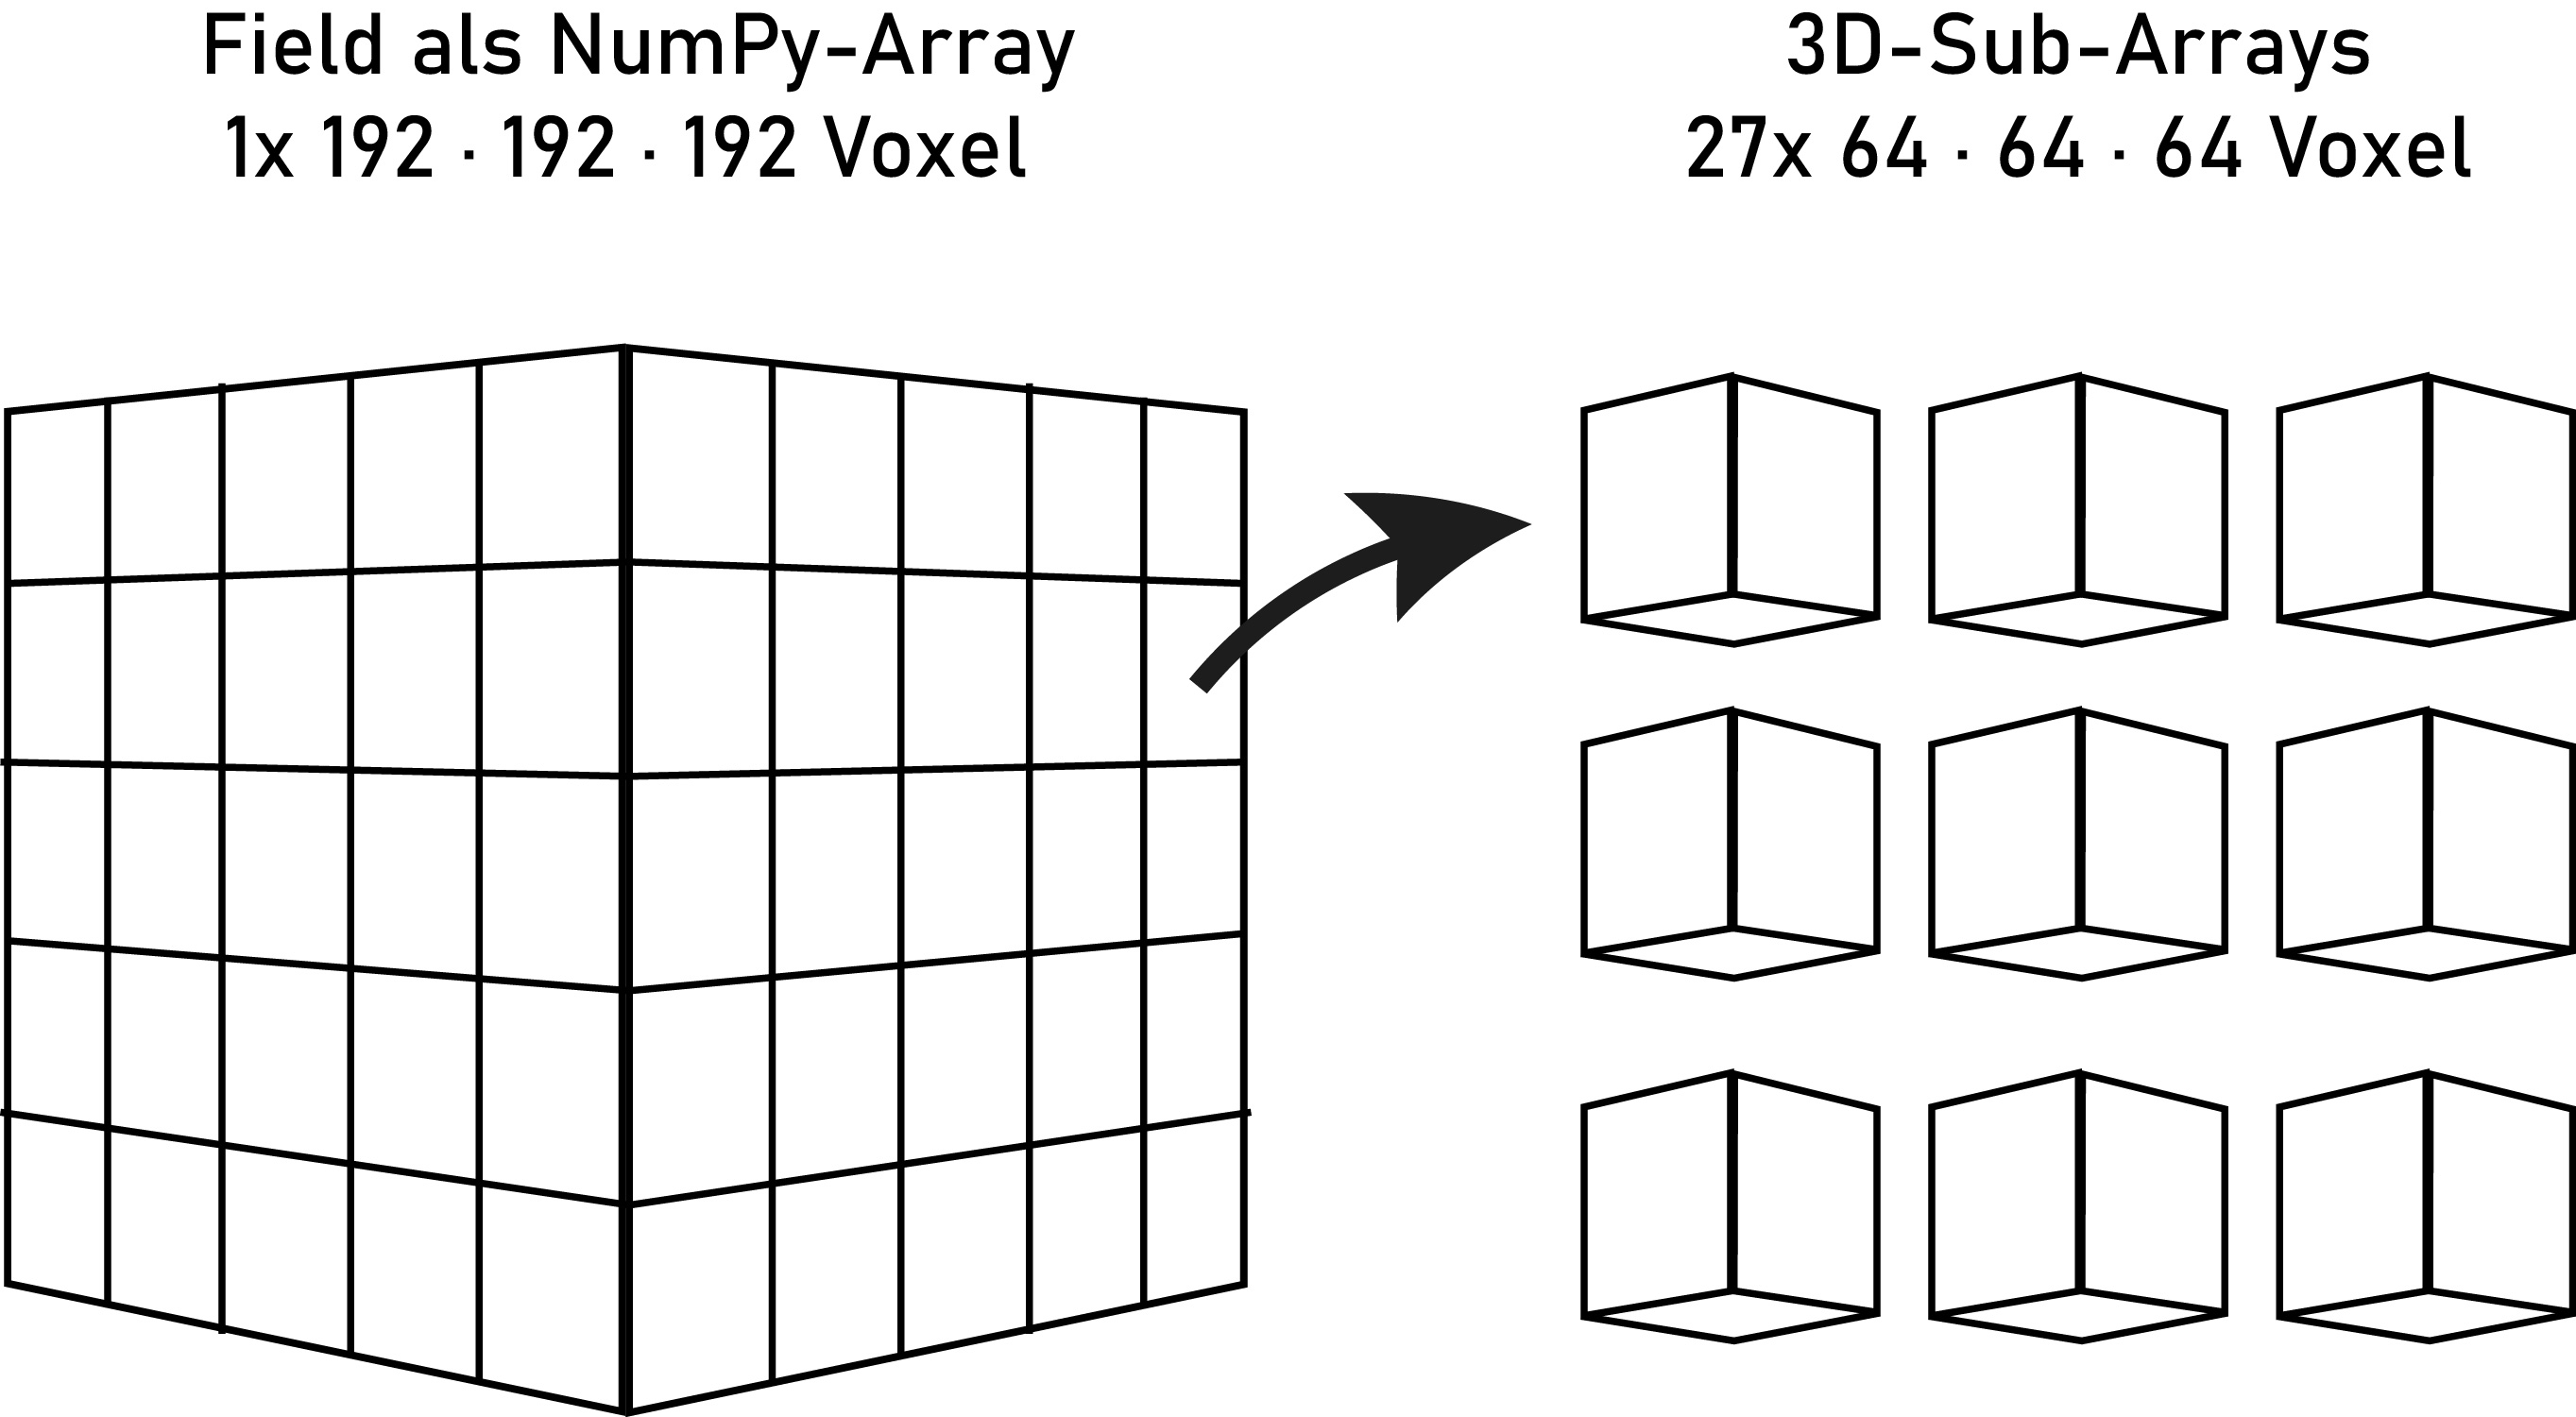
\includegraphics[width=11cm]{bilder/fieldarray.jpg}
    \caption{Umformung eines Fields in kleinere 3D-Sub-Arrays.}
    \source{Philipp Benner}
    \label{fieldarray}
\end{figure}


Somit ergab sich eine Anzahl von insgesamt 1620 einzelnen 3D-Sub-Arrays oder 810 Density und Temperature Paaren. Um auf der Grafikkarte trainieren zu können, konnten nicht alle 27 3D-Sub-Arrays eines Fields genutzt werden. Es wurden anstatt alle 27 Density und Temperature Field Paare eines Frames, nur jeweils ein Field-Paar pro Frame-Paket genutzt. Eine zufällige Selektion wählte  zehn Frame-Pakete mit jeweils sechs 3D-Sub-Arrays bestehend aus den drei aufeinanderfolgenden Frames und deren Fields aus. Ein Batch enthielt somit 10 Frame-Pakete bestehend aus sechs 3D-Sub-Arrays der Frames und deren Fields, insgesamt 60 3D-Sub-Arrays oder 30 Field-Paare aus temporal kohärenten Frames. Die sechs 3D-Sub-Arrays wurden als Input-Daten für die Convolutional Layer der beiden Netzwerke genutzt. Hierbei entstand ein weiterer Unterschied zur tempoGAN-Implementierung. In dessen Implementierung wurden alle 3D-Sub-Arrays für das Training genutzt und somit konnte ein kompletter Frame durch den Diskriminator und den Generator geschleust werden. In dieser Implementierung hingegen konnte nur der Teil eines Frames durch das Netz geschleust werden.\\

Das Training begann mit echten Daten im Diskriminator und es wurde diesem mitgeteilt, dass die Klassifizierung 1,0 betragen solle. Dazu wurde der Batch durch den Diskriminator geleitet, dessen Fehlerwert berechnet und anschließend die Gewichte aktualisiert.\\

Danach begann das Training des Diskriminators auf Daten trainiert, deren Label 0,0 betrug. Dazu wurde ein neuer Batch mit denselben Dimensionen der LowRes-3D-Arrays basierend auf Noise erzeugt, um falsche Daten zu erzeugen. Der Generator skalierte diesen Batch im Anschluss auf eine höhere Auflösung und er durchlief danach den Diskriminator, der den Bach mit dem Wert 0,0 klassifizierte. Der Fehlerwert wurde berechnet und anschließend die Gewichte aktualisiert.\\

Da der Generator nicht mit sechs Input Channels von aufeinanderfolgenden Frames trainiert werden sollte, sondern nur mit zwei, musste der Batch vor dem Training des Generators umgeformt werden. Der Grund hierfür war, dass es bei einer späteren Implementierung in einer VFX Software möglich sein soll, einen einzelnen Frame anhand des Density und Temperature Fields in seiner Auflösung zu skalieren. Dabei sollen der vorherige und nächste Frame nicht berücksichtigt werden. Der bestehende Batch echter Daten wurde aufgebrochen und in sechs kleinere Batches unterteilt. Somit konnte aus jedem Frame-Paket jeweils ein einzelner Batch pro Frame erzeugt werden. Jeder Batch enthielt nun zwei 3D-Sub-Arrays mit jeweils einem Field. Es wurden anschließend anstatt ein Batch mit mehreren Frame-Paketen, einzelne Frames durch den Generator geschleust. Der Generator erzeugte aus zwei LowRes-3D-Arrays der Größe 16 $\cdot$ 16 $\cdot$ 16 einen Output aus zwei Arrays der Größe 64 $\cdot$ 64 $\cdot$ 64. Die sechs Paare der hochskalierten Arrays wurden nun wieder in einem Batch gebündelt, der die ursprüngliche Batch-Form besitzt. Dieser Batch durchlief den Diskriminator geschleust und mit dem Fehlerwert des Diskriminators wurden die Gewichte des Generators aktualisiert. \\

Es wurden vor jedem aktualisieren der Gewichte, der aktuelle Fehlerwert für die beiden Durchgänge des Diskriminators und den des Generators gespeichert, um die Genauigkeit des Netzes evaluieren zu können.\\

Das Netz konnte während des Trainings nicht mit Testdaten getestet werden, da nicht ausreichend Speicher innerhalb der Grafikkarte für diese Daten zur Verfügung stand.\\

\section{Ausgabe des Netzes}
Nach dem Training des Netzes, war es in der Lage zwei Input-Arrays der Größe 16 $\cdot$ 16 $\cdot$ 16 auf die Größe 64 $\cdot$ 64 $\cdot$ 64 zu skalieren. Dies entspricht einem Faktor von vier für jede Dimension und 64 Mal mehr Voxel insgesamt. Um einen kompletten Frame einer Simulation im OpenVDB Format mithilfe der KI zu skalieren, musste der Frame mittels des Python-Skripts in ein 3D-NumPy-Array konvertiert und anschließend in einzelne 3D-Sub-Arrays aufgeteilt werden. Nach dem Konvertieren der 3D-Sub-Arrays in LowRes-3D-Arrays wurden diese durch den Generator schleust und er erzeugte eine skalierte Version. Anschließend durchliefen die einzelnen 3D-Sub-Arrays eine Umformung zu einem großen Array und es folgte eine Konvertierung zurück ins OpenVDB Format. 
%    \chapter{Ergebnisse}
\thispagestyle{fancy}

Im Folgenden sollen die Ergebnisse des KI-Modells nach den Gütekriterien evaluiert werden. Es wurden verschiedene Programme zur Analyse der Daten genutzt. Die grafische Aufbereitung der beim Training erfassten Fehlerwerte wurde mit der Software \textit{TensorBoard} \parencite{TensorBoard} durchgeführt. Statistiken entstanden in Python mittels der \textit{Pandas} \parencite{reback2020pandas} Programmbibliothek. 3D-Simulationsdaten verarbeiteten die Python-Module NumPy und OpenVDB. Für die visuelle Evaluation kam Houdini zum Einsatz. Es wurden insgesamt 23 Trainingsversuche durchgeführt und die Daten der letzten drei Trainingsversuche verglichen. Da diese ähnliche Graphen und Fehlerwerte erzeugten, bezieht sich die nachfolgende Evaluation nur auf den letzten Trainingsdurchlauf des KI-Modells.

\section{Evaluation der Gütekriterien}

\subsection{Artefaktfreiheit} Um die Ausgabe des Netzes auf visuelle Artefakte zu untersuchen, wurde eine neue, nicht im Training verwendete Simulation erzeugt. Es kam  dieselbe Vorgehensweise, wie für die Erzeugung der Trainingsdaten zum Einsatz. Die Simulation wurde erneut in 3D-Sub-Arrays und LowRes-3D-Arrays zerlegt, um eine niedrig aufgelöste Version zu erzeugen. Diese wurde anhand des trainierten KI-Modells hochskaliert und in ein OpenVDB konvertiert, um die Ursprungsgröße der Simulation zu erhalten. In Abbildung \ref{frame80}, einer Seitenansicht der Simulation, ist auf der rechten Seite die in Houdini erzeugte Simulation zu sehen und auf der linken Seite die durch die KI hochskalierte Version. Wie eindeutig zu erkennen, war das KI-Modell nicht in der Lage eine artefaktfreie Ausgabe zu erzeugen. Es generierte stattdessen eine Vielzahl an neuer Artefakte, wie etwa sich wiederholende Striche, welche rasterartig angeordnet sind. Ebenfalls waren einzelne, frei stehende Punkte sichtbar, die bei einer physikalisch korrekten Simulation nicht auftreten. Das Netz erzeugte eine gänzlich neue Form der Simulation, die nicht vergleichbar mit ihrem Ursprung ist.\\

\begin{figure}[ht]
    \centering
    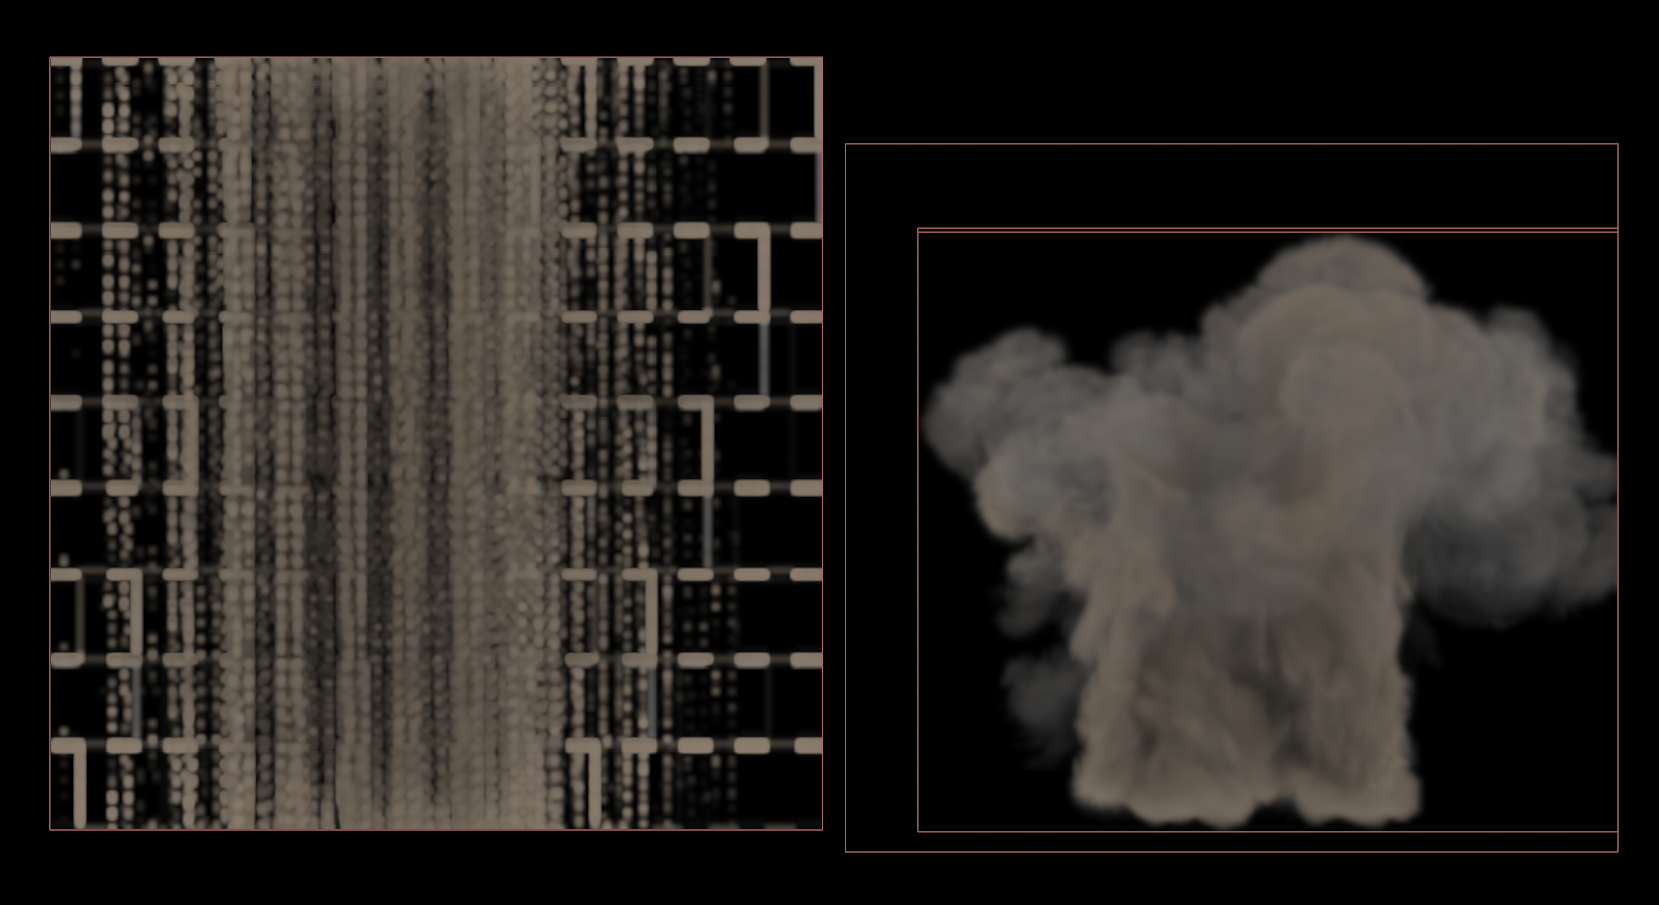
\includegraphics[width=14cm]{bilder/2Frame80.PNG}
    \caption{Detailansicht von Frame 80 der Simulationsvariante 2.}
    \source{Philipp Benner}
    \label{frame80}
\end{figure}

Das Kriterium der temporalen Kohärenz der Frames konnte ebenfalls nicht erfüllt werden, da einige Artefakte in jedem Frame an derselben Stelle sind. In Abbildung \ref{2scaled} ist der zeitliche Verlauf von zwei Simulationsvarianten zu sehen. Dargestellt sind jeweils Frame 1, Frame 40 und Frame 80. Sichtbar ist auch ein sich fortbewegender Streifen an dichten Voxeln, der über den Verlauf der Simulation von links nach rechts wanderte. Diese Form der Artefakte zeigte sich für alle getesteten Simulationsvarianten. \\

\begin{figure}[ht]
    \centering
    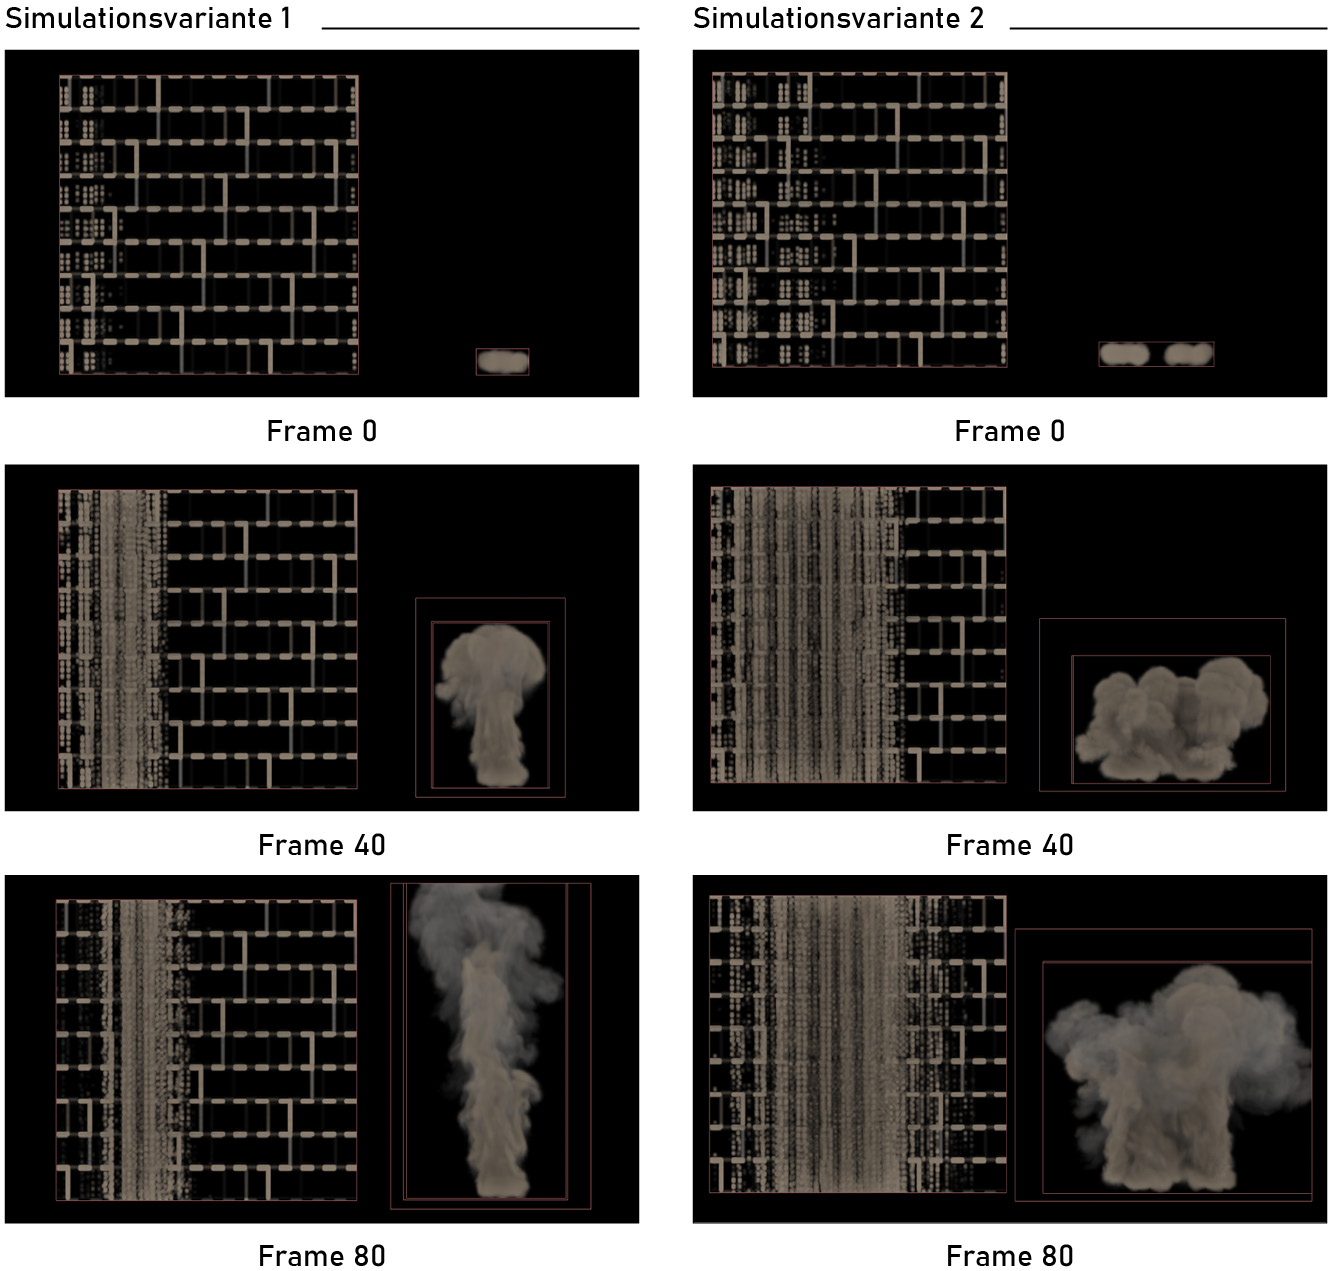
\includegraphics[width=13cm]{bilder/2_scaled_sims2.jpg}
    \caption{Vergleich einer Simulation mit einer hochskalierten Version derselben Simulation über die Zeit von 80 Frames.}
    \source{Philipp Benner}
    \label{2scaled}
\end{figure}
Hier zeigte sich das Problem des Mode Collapse, da das Netz eine ähnliche Ausgabe für jeden Frame erzeugte. Trotzdem ist sichtbar, dass das Netz trotz seiner Fehlerhaftigkeit in der Lage war, temporale Unterschiede zu erzeugen. Ein Grund für den Mode Collapse war möglicherweise die zufällige Selektion der 3D-Sub-Arrays. Da beim Training nicht alle Teile eines Frames verwendet wurden, war es möglich, dass viele Arrays durch den Discriminator und Generator geschleust wurden, die aus einer hohen Anzahl an Null-Werten bestanden. Das Netz war also nicht in der Lage eine physikalische Beziehung zwischen Density und Temperature Werten zu erlernen, da aussagekräftige Daten fehlten. Um dieses Problem zu lösen, müssten alle Teile eines Frames im Batch enthalten sein und nicht eine zufällige Auswahl an 3D-Sub-Arrays.\\

In Abbildung \ref{tensorboard} sind die Fehlerwerte oder Loss des Discriminators und Generators zu sehen. Sie waren das Ergebnis des Optimizers nach dem Training. Zur Messung der Fehlerwerte des Generators wurden echte sowie künstliche Daten durch den Generator geschleust und dessen Output anschließend vom Discriminator klassifiziert. Für die linken Graphen der Abbildung \ref{tensorboard} stellt die \textit{y}-Achse der Fehlerwert und die \textit{x}-Achse die Anzahl an trainierten Batches dar. Zu sehen ist ebenfalls, dass nur circa 1400 Batches trainiert wurden. Der Grund hierfür ist, dass sich früh abzeichnete, dass das Netz nicht optimal trainiert und deshalb das Training abgebrochen wurde. Der Generator erzeugte beispielsweise einen Fehlerwert von unter 0,1 innerhalb der ersten 200 Batches. Das drückt aus, dass sich der Discriminator sehr sicher ist, künstliche Daten klassifiziert zu haben. In diesem frühen Stadium des Trainings sind extreme Werte zur Klassifizierung ein Zeichen für ein schlecht trainierendes Netz. Die rechte Spalte der Abbildung \ref{tensorboard} zeigt auf ihrer y-Achse die Werte am Ausgang des Discriminators, basierend auf seinen Input-Daten. Dieser Wert unterscheidet sich dahingehend vom Fehlerwert, als dass er nicht das Ergebnis des Optimizers war, sondern der reine Output am letzten Layer des Modells. Die \textit{x}-Achse stellt die Anzahl der trainierten Batches dar. \\

\begin{figure}[ht]
    \centering
    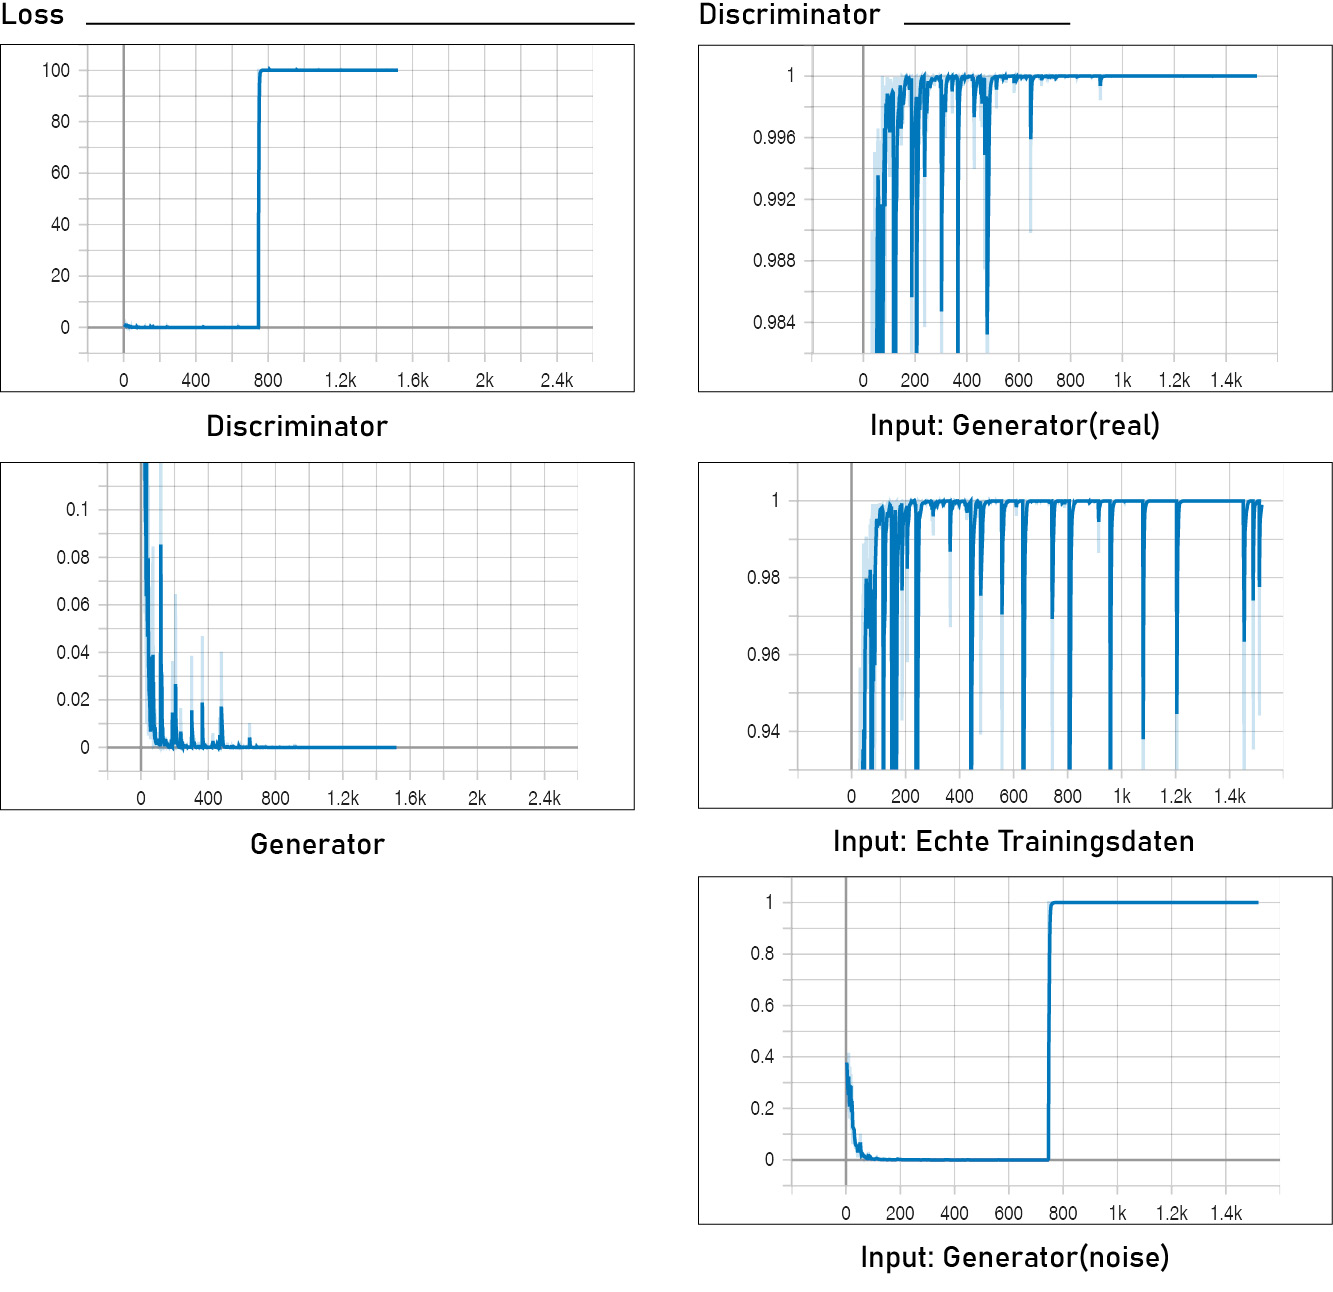
\includegraphics[width=13cm]{bilder/tensorboard2.jpg}
    \caption{Fehlerwerte des Generators und Discriminators.}
    \source{Philipp Benner}
    \label{tensorboard}
\end{figure}

Der obere, rechte Graph zeigt den Wert des Discriminators, wenn ihm ein Generator-Output gezeigt wurde, der mit echten Daten im Generator erzeugt wurde. Hier erreichen die Werte nach wenigen Batches einen Wert nahe 1, was bedeuten würde, dass der Generator optimal trainieren konnte, da der Discriminator sich sicher ist, echte Daten zu erkennen. Nach kurzer Trainingsdauer ist dies ebenfalls kein optimales Ergebnis.\\

Im mittleren Graphen zeigt sich die Entwicklung des Discriminators, als er direkt mit echten Daten trainiert wurde und nicht über den Output des Generators. Hier zeigte sich ebenfalls das Problem der extremen Werte in einem frühen Stadium des Trainings. Über den Verlauf des Trainings werden hier Einbrüche des Wertes im Graphen sichtbar.Diese bedeuten, dass sich der Discriminator bei einigen Batches nicht sicher war, ob die Daten echt sind. \\

Der untere Graph gibt den Wert des Discriminators an, als an diesen falsche Daten aus dem Generator angelegt wurden. Diese Daten wurden mit einem Noise erzeugt, dass der Generator hochskalierte. Erneut ist zu sehen, dass sich der Discriminator sehr früh sicher war, diese Daten als falsch klassifizieren zu können. Nach circa 750 Batches steigt der Wert jedoch auf nahezu 1,0. Dieser Sprung zeigt sich auch im Graphen für den Loss des Discriminators. Ein Vergleich mit den anderen Graphen zeigte, dass circa nach dem 750. Batch eine Veränderung im Generator auftrat. Der mittlere Graph der rechten Spalte zeigt keine sprunghafte Veränderung seiner Werte nach diesem Zeitpunkt, da dieser nicht auf dem Output des Generators basierte. Möglicherweise stellt dies den Zeitpunkt des Mode Collapse dar und der Generator lernte einen Output zu erzeugen, der stets mit annähernd 1,0 klassifiziert werden konnte. Ein Punkt, der diese Behauptung stützt, sind die sichtbaren, zufälligen Artefakte, die in Abbildung \ref{frame80} zu sehen sind.\\

Es lässt sich somit festhalten, dass das Kriterium der Artefaktfreiheit nicht erfüllt werden konnte.

\subsection{Formgleichheit} Das Kriterium der Formgleichheit ist ebenfalls nicht erfüllt, da aus den im Abschnitt zur Artefaktfreiheit genannten Gründen kein visuell korrekter Output erzeugt werden konnte. Die Form der Output-Simulation ist, wie in Abbildung \ref{frame80}, nicht mit ihrer Ursprungsform vergleichbar.\\

\subsection{Schnelligkeit}
Zur Evaluation der Schnelligkeit wurden, basierend auf den vorherigen Prozessen zu Erstellung von Trainingsdaten, drei neue Varianten an Simulationen in Houdini erzeugt. Jede Simulation bestand aus 80 Frames, die zu einem NumPy-Array der Auflösung 208 $\cdot$ 208 $\cdot$ 208 $\cdot$ Voxel konvertiert und in eine Low Resolution Version gewandelt wurden, anschließend mit dem KI-Modell hochskaliert und in das OpenVDB Format konvertiert, um die ursprüngliche Simulation wiederherzustellen.\\

Die Zeit, um eine Low Resolution Version aus einer Simulation zu erzeugen, sei zu vernachlässigen, da Tests zeigten, dass die Interpolation zu einer geringeren Auflösung hin circa eine Millisekunde betrug.\\

Es wurde anhand eines Python-Skripts analysiert, zu welchem Zeitpunkt ein Frame der originalen Simulation und ein Frame der KI-Skalierung erstellt wurde. Anhand von diesen Werten ließ sich ableiten, wie lange es dauerte, eine komplette Simulation in Houdini zu simulieren und ebenso die Zeit messen, die das KI-Modell zum Skalieren aller Frames benötigte. Ein Python-Skript berechnete ebenfalls die benötigte Zeit über alle Frames, da die anfänglichen Frames in Houdini weniger Zeit für die Simulation benötigen, als die Frames am Ende. Diese ersten Frames bestanden aus einer geringeren Anzahl an aktiven Voxeln in der Simulation. Somit mussten weniger Berechnungen am zu Beginn durchgeführt werden. In den Tabellen \ref{tab:speed} sind die gesamte Simulations- und Upsampling-Zeit und die durchschnittliche Dauer pro Frame von Houdini und des KI-Modells zu sehen. In der letzten Zeile wurde der Gesamtdurchschnitt der drei Werte gebildet. \\

\begin{table}[h]
    \centering
    \caption{Vergleich der Durchschnittsdauer eines simulierten und eines hochskalierten Frames.}
\begin{tabular}{|r|c|c|}
    
\hline
   & \multicolumn{2}{c|}{Houdini} \\
   \hline
           &  Simulationsdauer [s]       & 	$\varnothing$ Dauer pro Frame [s]\\
            \hline
Variante 1 & 29 Sek.          & 0,36 Sek.                       \\
Variante 2 & 19 Sek.          & 0,24 Sek.                      \\
Variante 3 & 21 Sek.           & 0,26 Sek.                       \\
\hline
\hline
 $\varnothing$   &     23 Sek.      &  0,27 Sek.           \\
 \hline
\end{tabular}
\vspace{0.7cm}\\
\begin{tabular}{|r|c|c|}
    
\hline
   &\multicolumn{2}{c|}{Upsampling} \\
   \hline
            & Dauer [s]      & 	$\varnothing$ Dauer pro Frame [s]        \\
            \hline
Variante 1     &  1 Min. 18 Sek.         & 0,97 Sek.             \\
Variante 2         &   1 Min. 12 Sek.        &  0,90 Sek.            \\
Variante 3          &  1 Min. 13 Sek.         &  0,91 Sek.           \\
\hline
\hline
 $\varnothing$   &    1 Min. 14 Sek.       &    0,93 Sek.    \\
 \hline
\end{tabular}

    \label{tab:speed}
\end{table}

Der Tabelle \ref{tab:speed} ist zu entnehmen, dass es etwa um den Faktor drei schneller war, einen Frame in Houdini zu simulieren, anstatt diesen mit dem KI-Modell zu skalieren. Dieser Zeitvorteil entsteht, da Houdini nicht jeden Voxel innerhalb des 3D-Arrays berechnete, sondern nur aktive Voxel mit Density und Temperature Werten \parencite{sidefxsparse}. Das KI-Modell hingegen hatte die Form eins 3D-NumPy-Arrays, dessen Werte alle in Input-Neuronen gewandelt werden mussten. Somit führte das KI-Modell immer eine Berechnung für die komplette Größe des Arrays durch und benötigte deshalb mehr Zeit.\\

Trotzdem ist es möglich, die Simulation schneller zu skalieren, als sie mit Houdini zu simulieren. Das KI-Modell hat den Vorteil, dass es parallel alle Frames zur selben Zeit skalieren kann. Dazu müssten mehrere Programminstanzen des Python-Skripts erstellt werden und jede Instanz würde einen Frame skalieren. Da das KI-Modell eine leistungsfähige, NVIDIA Grafikkarte pro Instanz benötigt, ist dieses Vorgehen beispielsweise nur auf einer Rechenfarm mit mehreren Grafikkarten möglich. Basierend auf den Werten aus Tabelle \ref{tab:speed} ließe sich die Simulationsvariante 1 ab vier Programminstanzen schneller hochskalieren, als Houdini durchschnittlich an Simulationszeit benötigt. Wie im Abschnitt zu Simulationen erläutert wurde, simuliert Houdini alle Frames nacheinander, da die Berechnungen eines Frames auf dem vorhergehenden Frame basieren. Diese Methode lässt sich nicht durch mehrere Houdini-Instanzen aufteilen.\\

Das Kriterium der Schnelligkeit ist somit erfüllt, sofern das KI-Modell zur parallelen Erzeugung von Frames genutzt wird.

\subsection{Datensparsamkeit}
Ob das Netz in die Fähigkeit hat, ein korrektes Upsampling von Simulationen mit dem Density und Temperature Field einer Simulation durchzuführen, ließ sich nicht evaluieren, da keine visuell korrekte Ausgabe erzeugt werden konnte. Somit ist das Kriterium der Datensparsamkeit nicht erfüllt.

\section{Vergleich mit tempoGAN}
Die Autoren der tempoGAN Implementierung zeigten jedoch, dass es durchaus möglich ist ein visuell artefaktfreies Upsampling über neuronale Netze zu erreichen \parencite[S. 95:10]{xie2018tempoGAN}. Die dort erzeugten Ergebnisse des Upsampling zeigten eine hohe zeitliche Kohärenz und einen sichtbaren Detailgrad in den Simulationen der erhöhten Auflösung.\\

Bei einer Evaluation der temoGAN Implementierung mit den Gütekriterien dieser Forschungsarbeit, ließe sich ein positives Ergebnis für die Artefaktfreiheit und Formgleichheit festhalten. Das Upsampling im tempoGAN Modell ist ebenso in einer hohen Geschwindigkeit möglich. Laut den Autoren dauerte die Simulation eines Frames in Mantaflow circa 31,5 Minuten, wohingegen das Upsampling des Low Resolution Frames durch das Netz nur 3,9 Minuten dauerte \parencite[S. 95:13]{xie2018tempoGAN}. \\

Ohne weitere Experimente lässt sich dieses Kriterium im VFX-Bereich nicht eindeutig testen, jedoch bietet es einen weiteren Forschungsanreiz.\\

Das Kriterium der Datensparsamkeit konnte durch die tempoGAN Implementierung nicht erfüllt werden, da dort das Velocity anstatt des Temperature Fields eingesetzt wurde. Wie in Tabelle \ref{tab:veltemp} gezeigt, benötigte die Kombination aus Density und Velocity Field mehr Speicherplatz als das Density und Temperature Field.

\section{Fazit und Lösungsansatz}
Die Evaluation der Gütekriterien zeigte, dass es nicht möglich war ein optimales KI-Modell für das Upsampling von Rauchsimulationen, basierend auf der Forschungsfrage, zu trainieren. Die Gründe hierfür sind vielseitig und ließen sich nicht an einer einzelnen Fehlerquelle festmachen. Jedoch lässt sich eine Artefaktfreiheit und die temporale Kohärenz mit weiterer Forschung erreichen, da eine Optimierung des KI-Modells ist durchaus möglich ist. \\

Optimierungsansätze liegen beispielsweise in der Batch Size und Hardwareleistung. Auf einer Grafikkarte, die über mehr Speicherplatz verfügt, ließen sich alle Frames durch das Netz schleusen, anstatt nur eine Selektion an 3D-Sub-Arrays. Ebenfalls ließe sich das KI-Modell auf einer Farm trainieren, auf der möglicherweise mehr als ein Frame Teil eines Batches sein könnte oder es ließen sich mehr Trainingsepochen in kürzerer Zeit realisieren. Eine weitere Möglichkeit zur Optimierung liegt im Aufbau des Discriminators und des Generators. Wie im Abschnitt der Implementierung des Generators beschrieben, wurden für diesen mehr Convolutional und Residual Layer verwendet als beim Discriminator. Dadurch entstand das Problem, dass die beiden Kontrahenten nicht gleich stark und der Generator überlegen war. Er erhielt vom Discriminator kein ausreichendes Feedback, um sich in einer Weise zu verbessern, die visuell artefaktfreie Ergebnisse erzeugt.\\

Die Ergebnisse der tempoGAN Implementierung zeigen aber deutlich, dass ein Upsampling mittels neuronaler Netze möglich ist. Da die Autoren den Quellcode offengelegt und den Aufbau des KI-Models sehr genau beschrieben haben, kann dieses KI-Modell mit weiterer Entwicklung in eine Software des VFX-Bereichs integriert werden. Ein Mittel dafür stellt das Python-Modul des OpenVDB Herstellers dar, da dieses die Datenkonvertierung zwischen OpenVDB und einem NumPy-Array stark vereinfacht. Somit ließen sich diverse Python-Skripte in Houdini implementieren, die eine solche Aufgabe übernehmen könnten.
%    \chapter{Ausblick}
\thispagestyle{fancy}

In dieser Arbeit wurde aufzeigt, dass eine generelle Implementierung von neuronalen Netzen im Bereich der 3D-Simulationen für VFX möglich ist. Eine große Herausforderung war jedoch die Verarbeitung der Daten und das stabile Trainieren eines KI-Modells. Hier ergab sich Potenzial für zukünftige Studien, die sich der Vereinfachung des OpenVDB-NumPy-PyTorch Workflows widmen oder an einer Lösung für eine variierende Input-Anzahl in neuronalen Netzen forschen. Da das OpenVDB Dateiformat nur aktive Voxel speichert und sich die Auflösung jeder Dimension pro Frame ändern kann, würde eine variierende Input-Anzahl eine Simplifizierung in der Datenverarbeitung darstellen.\\

Ebenfalls blieb die Frage offen, ob ein neuronales Netz anhand des Density und Temperature Fields ein visuell artefaktfreies Ergebnis beim Upsampling erzielen könnte und ob es in der Lage wäre, eine physikalische Verbindung zwischen diesen beiden Fields zu erkennen. Dem schließt sich die Frage an, ob ein neuronales Netz, das auf einem Datensatz von Simulationen einer Explosion zufriedenstellend trainiert wurde, ebenso gute Ergebnisse erzeugen könnte, wie wenn es dazu genutzt werden würde, die Rauchsimulation einer Kerze zu skalieren. \\
Weitere Forschungsbereiche ergeben sich innerhalb der verschiedenen Programme zur Erzeugung von Rauchsimulationen. Anstatt die Berechnungen für den nächsten Frame einer Simulation auf den Voxeln zu basieren, ließen sich eventuell die Parameter in ein neuronales Netz schleusen, die für die Berechnung der Voxel zuständig sind. Möglicherweise ist ein neuronales Netz so in der Lage Werte für Formeln und Zeitintervalle von physikalischen Strömungen als Input zu erhalten und erzeugt darauf basierend einen Frame bestehend aus Voxeln. \\

Allgemein bleiben Rauchsimulationen ein Forschungsgebiet, das einige Forschungspotentiale für Effizienzsteigerung bietet. Die Möglichkeit Simulationen schneller durchzuführen oder sie auf andere Weise mit neuronalen Netzen zu manipulieren, kann finanzielle Vorteile für ein Unternehmen oder mehr kreative Freiheit für einen 3D-Artist bedeuten. Mit steigender Leistungsfähigkeit von Computerhardware kann es in Zukunft möglich sein, die Dauer solcher Forschungen zu verkürzen und sie allgemein zugänglicher zu machen. Somit entstehen eine Vielzahl neuer Anwendungen, die Arbeitsabläufe beschleunigen und die Arbeit eines Artists vereinfachen können.
%    \chapter*{Anhang}
\thispagestyle{plain}
\addcontentsline{toc}{chapter}{Anhang}

\section{Aufbau des Generators}
\begin{python}
Generator(
(block1): Sequential(
(0): Conv3d(2, 4, kernel_size=(5, 5, 5), stride=(1, 1, 1), padding=(2, 2, 2))
(1): BatchNorm3d(4, eps=1e-05, momentum=0.1, affine=True, track_running_stats=True)
(2): ReLU(inplace=True)
(3): Conv3d(4, 4, kernel_size=(5, 5, 5), stride=(1, 1, 1), padding=(2, 2, 2))
(4): BatchNorm3d(4, eps=1e-05, momentum=0.1, affine=True, track_running_stats=True)
)
(shortcut1): Sequential(
(0): Conv3d(2, 4, kernel_size=(1, 1, 1), stride=(1, 1, 1))
(1): BatchNorm3d(4, eps=1e-05, momentum=0.1, affine=True, track_running_stats=True)
)
(block2): Sequential(
(0): Conv3d(4, 8, kernel_size=(5, 5, 5), stride=(1, 1, 1), padding=(2, 2, 2))
(1): BatchNorm3d(8, eps=1e-05, momentum=0.1, affine=True, track_running_stats=True)
(2): ReLU(inplace=True)
(3): Conv3d(8, 2, kernel_size=(5, 5, 5), stride=(1, 1, 1), padding=(2, 2, 2))
(4): BatchNorm3d(2, eps=1e-05, momentum=0.1, affine=True, track_running_stats=True)
)
(shortcut2): Sequential(
(0): Conv3d(4, 2, kernel_size=(1, 1, 1), stride=(1, 1, 1))
(1): BatchNorm3d(2, eps=1e-05, momentum=0.1, affine=True, track_running_stats=True)
)
(r1): ReLU(inplace=True)
(r2): ReLU(inplace=True)
(u1): Upsample(size=(32, 32, 32), mode=nearest)
(u2): Upsample(size=(64, 64, 64), mode=nearest)
)
\end{python}
\newpage
\thispagestyle{plain}
\section{Aufbau des Discriminators}
\begin{python}
Discriminator(
(main): Sequential(
(0): Conv3d(6, 8, kernel_size=(4, 4, 4), stride=(1, 1, 1), bias=False)
(1): BatchNorm3d(8, eps=1e-05, momentum=0.1, affine=True, track_running_stats=True)
(2): LeakyReLU(negative_slope=0.01, inplace=True)
(3): Conv3d(8, 16, kernel_size=(4, 4, 4), stride=(1, 1, 1), bias=False)
(4): BatchNorm3d(16, eps=1e-05, momentum=0.1, affine=True, track_running_stats=True)
(5): LeakyReLU(negative_slope=0.01, inplace=True)
(6): Conv3d(16, 1, kernel_size=(4, 4, 4), stride=(1, 1, 1), padding=(2, 2, 2), bias=False)
(7): Flatten(start_dim=1, end_dim=-1)
(8): LazyLinear(in_features=0, out_features=1, bias=True)
(9): Sigmoid()
)
)
\end{python}

\thispagestyle{fancy}
\chapter{Vorwort}
\chapter{Überblick}

\section{Herausforderungen bei der Selbstevaluation des \\ Startup-Fortschritts}
\section{Bedeutung des Design Thinking-Prozesses für Startups}

\section{Relevanz eines strukturierten Reifegradmodells}
\section{Fehlende standardisierte Methode zur \\ Startup-Selbsteinschätzung}
\chapter{Ziele}

\section{Entwicklung eines adaptiven Fragebogens zur Evaluation des Design Thinking-Prozesses eines Startups}
\section{Forschungsfragen}


\chapter{Theoretische Grundlagen}

\section{Grundlagen des Design Thinking-Prozesses}
\subsection{Definition und Phasen des Design Thinking}
\subsection{Unterschiede zu anderen Innovationsmethoden}
\subsubsection{Lean Startup}
\subsubsection{Weitere Methoden}

\section{Reifegradmodelle in der Startup-Forschung}
\subsection{Bestehende Reifegradmodelle}
\subsubsection{Schwächen dieser Modelle}
\subsection{Anforderungen an ein praxistaugliches Reifegradmodell für Startups}

\section{Fragebögen zur Selbsteinschätzung}
\subsection{Grundlagen zu Fragebögen mit Selbstkontrolle}
\subsubsection{Kombination aus qualitativen und quantitativen Fragen}
\subsection{Adaptive Fragebogen-Systeme: Dynamische Anpassung der Fragen}
\subsubsection{Gezielte Rückfragen}
\subsection{Definition von Metriken zur Startup-Evaluation}

\chapter{Stand der Forschung}

\chapter{Methodik}

\section{Experteninterviews zur Identifikation von Selbstüberschätzung}
\section{Entwicklung eines Fragebogens mit und ohne adaptive Nachfragen}
\section{Evaluation durch  Befragungsrunden mit Startups}

\chapter{Entwicklung des Fragebogens}

\section{Anforderungen an den Fragebogen}
\subsection{Strukturierte Erfassung des Design Thinking-Fortschritts}
\subsection{Kriterien für die Formulierung von Fragen und Antwortoptionen}

\section{Dynamische Anpassung der Fragen}
\subsection{Konzept eines adaptiven Fragebogens}
\subsection{Definition von Regeln für Folgefragen und Feedback-Mechanismen}

\section{Technische Umsetzung als Web-Tool}
\subsection{Architektur des webbasierten Fragebogens}
\subsection{Technologien und Frameworks für die Entwicklung}

\chapter{Evaluation und Analyse}

\section{Testphase mit Startups}
\subsection{Durchführung des Fragebogens mit Startup-Teams}
\subsection{Datenerhebung}

\section{Auswertung der Ergebnisse}
\subsection{Analyse der erfassten Daten}

\section{Vergleich mit bestehenden Methoden}
\subsection{Diskussion der Vorteile des entwickelten Modells im Vergleich zu bestehenden Ansätzen}

\chapter{Fazit und Ausblick}

\section{Zusammenfassung der Erkenntnisse}
\subsection{Bedeutung adaptiver Fragebögen für \\ Startup-Selbsteinschätzungen}
\subsection{Potenzial von Reifegradmodellen im Design Thinking-Kontext}

\section{Limitationen der Arbeit}
\subsection{Herausforderungen bei der Messung subjektiver Einschätzungen}
\subsection{Mögliche Verzerrungen durch Selbstauskunft}

\section{Zukünftige Forschungsansätze}
\subsection{Weiterentwicklung des Fragebogens durch Machine Learning}
\subsection{Anwendung des Modells auf andere Innovationsmethoden}
    \pagestyle{plain}
    
\thispagestyle{plain}
\addcontentsline{toc}{chapter}{Literaturverzeichnis}
\begingroup

  \let\clearpage\relax        % report
\printbibliography
\endgroup

    
\end{document}
